% Using template for a Computer Science Tripos Part II project dissertation
\documentclass[12pt,a4paper]{report}
\usepackage[pdfborder={0 0 0}]{hyperref}
\usepackage[margin=20mm]{geometry}
\usepackage{graphicx, caption}
\usepackage{docmute}   % only needed to allow inclusion of proposal.tex
\usepackage{natbib}
\usepackage{verbatim}
\usepackage{wasysym}
\usepackage{color}
\usepackage{float}
\usepackage{tikz}
\usepackage{hyperref}
\usepackage[capitalise, noabbrev]{cleveref}
\usepackage{stix} % different font
\usepackage{minted}

\usepackage{url}

\usepackage[utf8]{inputenc}
\usepackage{changepage}
\usepackage[euler]{textgreek}


\raggedbottom                           % try to avoid widows and orphans
\sloppy
\frenchspacing
\clubpenalty1000%
\widowpenalty1000%
\parindent 0pt
\parskip 6pt

\renewcommand{\baselinestretch}{1.1}    % adjust line spacing to make
                                        % more readable

\pagenumbering{roman}

\begin{document}
%TC:ignore

%%%%%%%%%%%%%%%%%%%%%%%%%%%%%%%%%%%%%%%%%%%%%%%%%%%%%%%%%%%%%%%%%%%%%%%%
% Title


\pagestyle{empty}

\rightline{\LARGE \textbf{Z\'ebulon Goriely}}
\vspace*{2mm}

\vspace*{60mm}
\begin{adjustwidth}{40pt}{40pt}
\begin{center}
\Huge
\textbf{Simulating Natural Language Learning and Evolution} \\[15mm]
\Large
Computer Science Tripos -- Part II \\[3mm]
Queens' College \\[3mm]
May 2020 \\[3mm]
\end{center}
\end{adjustwidth}

%%%%%%%%%%%%%%%%%%%%%%%%%%%%%%%%%%%%%%%%%%%%%%%%%%%%%%%%%%%%%%%%%%%%%%%%%%%%%%
% Proforma, table of contents and list of figures

\pagestyle{plain}

\newpage
\section*{Declaration of Originality}

I, Z\'ebulon Goriely of Queens' College, being a candidate for Part II of the Computer
Science Tripos, hereby declare
that this dissertation and the work described in it are my own work,
unaided except as may be specified below, and that the dissertation
does not contain material that has already been used to any substantial
extent for a comparable purpose.

I, Z\'ebulon Goriely of Queens' College, am content for my dissertation to be made available to the students and staff of the University.

\bigskip
\leftline{{\bf Signed:} Z\'ebulon Goriely}

\medskip
\leftline{{\bf Date:} \today}

\section*{Acknowledgements}

Thanks to Paula Buttery and Andrew Caines for supervising me, providing amazing feedback on my project and for giving me an incredible insight into the world of Computer Science research. Thank you to Alice Wenban for putting up with my enthusiasm about this project. Thank you to Alastair Beresford for Directing my Studies throughout the last three years and providing feedback on my work. Thank you to my parents for their continuous and constant support through my studies.
\\
\\
This work was performed using resources provided by the Cambridge Service for Data Driven Discovery (CSD3) operated by the University of Cambridge Research Computing Service (www.csd3.cam.ac.uk), provided by Dell EMC and Intel using Tier-2 funding from the Engineering and Physical Sciences Research Council (capital grant EP/P020259/1), and DiRAC funding from the Science and Technology Facilities Council (www.dirac.ac.uk).

\chapter*{Proforma}

{\large
\begin{tabular}{ll}
Candidate number:               & \bf 2049E???                       \\
Project Title:      & \bf Simulating Language Learning and Evolution \\
Examination:        & \bf Computer Science Tripos -- Part II, May 2020  \\
Word Count:         & \bf NULL\footnotemark[1]  \\
Final Line Count:         & \bf 3125 \footnotemark[2]  \\
Project Originator: & 2049E???                    \\
Project Supervisors:         & Prof. Paula Buttery and Dr. Andrew Caines                  \\ 
\end{tabular}
}
%\footnotetext[1]{This word count was computed
%by \texttt{detex diss.tex | tr -cd '0-9A-Za-z $\tt\backslash$n' | wc -w}
%}
\footnotetext[1]{This word count was computed using:
\texttt{texcount -subcount=chapter -merge -brief -sum diss.tex} with \texttt{\%TC:ignore} and \texttt{\%TC:endignore} around the appendices and front matter.
}
\footnotetext[2]{This line count was computed using: \texttt{cat \`{}find . -name ``*.py'' \`{} | wc -l}
}
\stepcounter{footnote}
\stepcounter{footnote}

\section*{Original Aims of the Project}

Language has evolved and therefore probably gave an evolutionary advantage to the individuals that exhibited it. According to \citet{Cangelosi1998}, it is difficult to investigate the evolutionary origin of language and the selective pressures that may have originated language due to the limited evidence available. In the referenced paper, they describe using a simulated world to investigate the effect of introducing language to a population of entities controlled by neural networks. These entities interact with an environment of mushrooms that are edible and poisonous and must correctly categorise them to survive. Exploring this simulation is the basis of my project.

\section*{Work Completed}

I successfully implemented the simulation; comparing three different populations. To simulate evolution, I implemented a genetic algorithm. Through algorithmic analysis, I discovered key optimisations. The state of the simulation was saved at each generation in order to: i) plot the fitness of the populations; ii) plot the quality of the language produced; iii) investigate behavioural tests. I compared these findings with \citet{Cangelosi1998} to confirm the evolutionary advantage of language. I then conducted my own analysis to determine the robustness of the simulation, criticise arbitrary decisions made by \citet{Cangelosi1998} and demonstrate a correlation between population behaviour and fitness.

\section*{Special Difficulties}

None.
 
\tableofcontents

\listoffigures

%%%%%%%%%%%%%%%%%%%%%%%%%%%%%%%%%%%%%%%%%%%%%%%%%%%%%%%%%%%%%%%%%%%%%%%
%%%%%%%%%%%%%%%%%%%%%%%%%%%%%%%%%%%%%%%%%%%%%%%%%%%%%%%%%%%%%%%%%%%%%%%
%%%%%%%%%%%%%%%%%%%%%%%%%%%%%%%%%%%%%%%%%%%%%%%%%%%%%%%%%%%%%%%%%%%%%%%
%%%%%%%%%%%%%%%%%%%%%%%%%%%%%%%%%%%%%%%%%%%%%%%%%%%%%%%%%%%%%%%%%%%%%%%
%%%%%%%%%%%%%%%%%%%%%%%%%%%%%%%%%%%%%%%%%%%%%%%%%%%%%%%%%%%%%%%%%%%%%%%
%%%%%%%%%%%%%%%%%%%%%%%%%%%%%%%%%%%%%%%%%%%%%%%%%%%%%%%%%%%%%%%%%%%%%%%
%%%%%%%%%%%%%%%%%%%%%%%%%%%%%%%%%%%%%%%%%%%%%%%%%%%%%%%%%%%%%%%%%%%%%%%
%%%%%%%%%%%%%%%%%%%%%%%%%%%%%%%%%%%%%%%%%%%%%%%%%%%%%%%%%%%%%%%%%%%%%%%
% Introduction

%TC:endignore

\pagestyle{headings}

\chapter{Introduction}
\pagenumbering{arabic}
\setcounter{page}{1}

Humans evolved to understand and produce language, and according to theories of natural selection we therefore infer that the ability to use language gave an evolutionary advantage to those individuals who exhibited it. The field of language evolution is diverse and spans many scientific disciplines, from evolutionary biology and neuroscience to psycholinguistics and cultural anthropology. One of the main problems with studying the evolution of language is the relative abundance of theories compared to the limited empirical evidence since anatomically-modern humans emerged in the fossil record 200,000 years ago \citep{Fleagle2008}. It is not known when, during or prior to this period, language actually emerged. To our knowledge, language evolution is a once-occurring, long-term and complex system making it very difficult to study, but computer simulations may provide a means by which to examine the theories surrounding it.

Computer simulations are \emph{``theories of the empirical phenomena that are simulated"} \citep{Cangelosi2002}. Simulations encompass the hypotheses of the theory and produce empirical predictions that can then be evaluated against known phenomena \citep{cavalli1997genes}. Simulations can act as virtual laboratories where impossible experiments (such as language evolution) can be run, controlling parameters that could never be controlled in real life, such as evolutionary or environmental factors. Simulations can also act as quantitative verifiers for the internal validity of vague and ambiguous theories, requiring explicit definitions of key assumptions. Finally, simulations can be used as a tool for studying complex systems. These are composed of many interacting entities that produce global properties that cannot be predicted even with complete knowledge of the system. A noteworthy example is Conway's Game of Life, a cellular automaton with very simple rules in which it is possible to build a universal Turing Machine \citep{rendell2002turing}.

Language itself is a complex system and it has been shown that the bottom-up approach of simulations can generate key insights \citep{langton1997artificial}. In this project, I will use simulation to explore the genetic advantage of populations of entities who exhibit language over those who do not.

\section{Prior Work}

Computer simulations have been applied to a variety of interesting questions in the field of language evolution. Seeking to investigate the emergence of syntactic universals, \citet{kirby2002emergence} presented the Iterated Learning Model (ILM), a means of simulating cultural transmission of language. They discuss the intersection of learning, cultural evolution and biological evolution as defining the emergence of language and use the ILM to explain the emergence of compositionality, irregularity and frequency properties of language.

To study the emergence of shared vowel systems, \citet{de1997generating} created a population-based language game model involving language games and genetic algorithms. He explores an apparent bias towards vowel systems that reflect the structure of human vowel systems, discussing how this is explained by the ``optimisation of acoustic distinctiveness'' from an information-theoretic perspective.

\citet{parisi2002unified} discuss the use of a single unified simulation for the investigation of research questions surrounding the evolution of language. In particular, \citet{Cangelosi1998} introduce the ``toy mushroom world'' simulation for investigating how the evolution of categorisation abilities is linked to the evolution of communication signals for distinguishing these categories. I choose to replicate this work because of one of the broad questions that it tackles: how language can evolve when it has a purely informative function and so is advantageous only to the receiver and not the producer. 

%In further papers, Cangelosi explores how this simulation can be made more complex by introducing cultural transmission of language and finds that in compositional languages with a verb-noun structure, verbs have a larger positive effect on the performance of the species \citep{cangelosi2001evolution}. As an extension to my core project I will investigate the effect of incorporating cultural transmission to my simulation. [TODO: DO THIS EXTENSION]

\section{Project Overview}

In my project I re-implement the ``toy mushroom world'' simulation described by \citet{Cangelosi1998}. This involved the following contributions:
\begin{itemize}
	\itemsep0em
	\item Researching relevant algorithms and data structures (Chapter 2).
	\item Taking a professional approach to managing my project (Chapter 2).
	\item Creating three populations of feed-forward neural networks from scratch (Chapter 3).
	\item Implementing the genetic algorithm used to evolve the populations (Chapter 3).
	\item Develop optimisations to reduce the time taken to run the simulation (Chapter 3).
	\item Creating a suite of data gathering tools, interactivity features and analysis methods (Chapter 3).
	\item Comparing the fitness of the populations and the languages they produce to the results of Cangelosi and Parisi (Chapter 4).
	\item Conducting original analysis of population behaviour and exploring the robustness of the simulation to parameter differences (Chapter 4).
	\item Discussing personal reflections and potential future work (Chapter 5).
\end{itemize}

%%%%%%%%%%%%%%%%%%%%%%%%%%%%%%%%%%%%%%%%%%%%%%%%%%%%%%%%%%%%%%%%%%%%%%%
%%%%%%%%%%%%%%%%%%%%%%%%%%%%%%%%%%%%%%%%%%%%%%%%%%%%%%%%%%%%%%%%%%%%%%%
%%%%%%%%%%%%%%%%%%%%%%%%%%%%%%%%%%%%%%%%%%%%%%%%%%%%%%%%%%%%%%%%%%%%%%%
%%%%%%%%%%%%%%%%%%%%%%%%%%%%%%%%%%%%%%%%%%%%%%%%%%%%%%%%%%%%%%%%%%%%%%%
%%%%%%%%%%%%%%%%%%%%%%%%%%%%%%%%%%%%%%%%%%%%%%%%%%%%%%%%%%%%%%%%%%%%%%%
%%%%%%%%%%%%%%%%%%%%%%%%%%%%%%%%%%%%%%%%%%%%%%%%%%%%%%%%%%%%%%%%%%%%%%%
%%%%%%%%%%%%%%%%%%%%%%%%%%%%%%%%%%%%%%%%%%%%%%%%%%%%%%%%%%%%%%%%%%%%%%%
%%%%%%%%%%%%%%%%%%%%%%%%%%%%%%%%%%%%%%%%%%%%%%%%%%%%%%%%%%%%%%%%%%%%%%%
% Preparation

\chapter{Preparation}\label{chapter:preparation}

\emph{This chapter covers the background to my project in Sections \ref{section:world} to \ref{section:analysis}, then evaluates the requirements for the project in \cref{section:requirements}. I discuss the starting point of my project in \cref{section:starting} and the software engineering techniques used in \cref{section:software}.}

\section{Mushroom World}\label{section:world}

To explore how the introduction of language may affect a population's fitness, we need a simulated environment in which to observe the effect of these changes. The ``mushroom world'' described by \cite{Cangelosi1998} was inspired by the use of signals to communicate information about food location and quality present in many species.

In the simulation, organisms are represented by \emph{entities}. The entities live in an environment populated by two different types of mushroom; edible and poisonous. The entities reproduce based on their ability to eat edible mushrooms and avoid the poisonous ones. They need to learn to categorise the two mushrooms and respond accordingly by moving towards and eating the edible mushrooms and moving away from the poisonous mushrooms.

To ensure this categorisation is not trivial for the entities, the mushrooms have different properties. Edible mushrooms resemble each other but are not identical and likewise for poisonous mushrooms.

Each entity will live in an environment of $20 \times 20$ cells containing 20 randomly distributed mushrooms; 10 of which are edible and 10 of which are poisonous. They are able to explore this world during 15 epochs of 50 simulation cycles each. Between each epoch the world is reset; the entity is placed again in a new environment with 20 new randomly distributed mushrooms. An example of this world can be seen in \cref{fig:environment}.

\begin{figure}[ht]
\centering
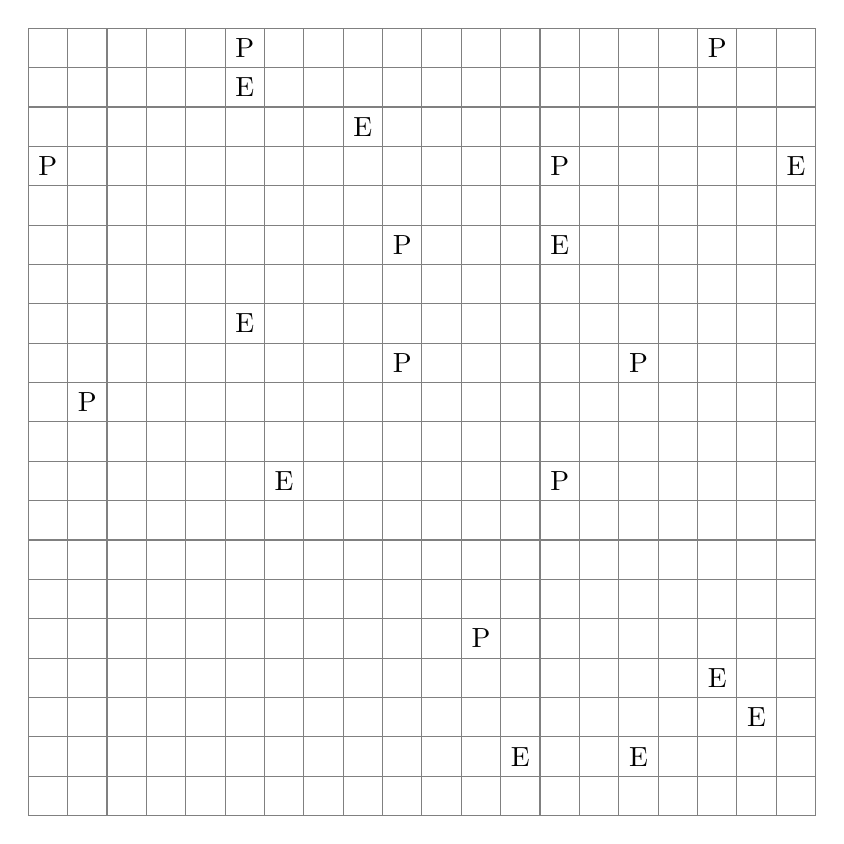
\begin{tikzpicture}
\draw[step=0.5cm,color=gray] (0,0) grid (10,10);
\node at (6.75,8.25){P};
\node at (5.75,2.25){P};
\node at (4.75,5.75){P};
\node at (6.75,4.25){P};
\node at (8.75,9.75){P};
\node at (4.75,7.25){P};
\node at (2.75,9.75){P};
\node at (0.25,8.25){P};
\node at (0.75,5.25){P};
\node at (7.75,5.75){P};
\node at (9.75,8.25){E};
\node at (2.75,9.25){E};
\node at (9.25,1.25){E};
\node at (8.75,1.75){E};
\node at (3.25,4.25){E};
\node at (2.75,6.25){E};
\node at (4.25,8.75){E};
\node at (6.75,7.25){E};
\node at (7.75,0.75){E};
\node at (6.25,0.75){E};
\node at (2.25,5.75){$\blacktriangle$};
\end{tikzpicture}
\caption{An entity ($\blacktriangle$) in the simulation environment with edible (E) and poisonous (P) mushrooms.}
\label{fig:environment}
\end{figure}
The constants chosen by Cangelosi and Parisi are fairly arbitrary. In later sections I will explore the effects of changing them, but for now I can intuitively explain some of these choices. The 15 epochs provide a large enough sample size of environments for entity behaviour to be significant. The 50 cycle constraint captures limited lifetimes, forcing entities to learn optimal strategies to maximise the number of edible mushrooms eaten. A full list of constants can be seen in \cref{table:constants}.

%The 15 epochs are used to average out the randomly generated positions of mushrooms so that it is really the behaviour of the entity that is being tested, not the random choice of environment. The 50 simulation cycles along with the specific dimensions of the environment ensure that the entity will likely be able to reach at least one edible mushroom but will likely not be able to eat all edible mushrooms in this time. This encourages productive strategies to search for edible mushrooms within the limited number of simulation cycles. Intuitively, this reflects the limited time that living entities have to search for food in their lifetimes. A full list of constants can be seen in \cref{table:constants}.

\section{Entities}\label{section:entities}

Entities can \emph{perceive} their surroundings and \emph{act} accordingly. Perception is composed of three senses; the entity can sense the \emph{direction} of the nearest mushroom (a `smelling' sense), can see the \emph{properties} of mushrooms it is adjacent to (a `visual' sense) and can receive \emph{signals} from other entities (an `auditory' sense). The adjacency restriction to the visual sense means that without additional signals, entities must approach mushrooms in order to be able to categorise them.

Action consists of two possible responses; the \emph{movement} of the entity and the \emph{signal} it produces. The movement is restricted to four options; moving one cell forwards, turning 90\textdegree~left, turning 90\textdegree~right and doing nothing. To eat a mushroom, the entity moves into the mushroom's cell. The signal is used to communicate information to other entities when we add language to the simulation.

The simulation should also incorporate evolution; some process by which the fittest entities of a species reproduce to pass on their behaviour to a new generation, with some degree of mutation. This will allow a population's average fitness to improve over many generations.

\subsection{Feed-Forward Neural Networks}\label{section:neural}

Consistent with \citet{Cangelosi1998}, I use \emph{Artificial Neural Networks} to model the entities. Neural networks are composed of nodes (artificial neurons) which loosely model the neurons in a biological brain. Each node processes an output signal by computing a non-linear function of the sum of inputs. By organising these nodes into layers, signals can travel through from the input layer to the output layer. This is a \emph{feed-forward} neural network as the signal flows forward through the layers (can't loop back). A \emph{fully-connected} neural network feeds the output of every node in a layer into the input of every node in the next layer. 

Each node calculates a weighted average of the inputs offset by a bias term. An \emph{activation function} can then be applied to produce the output of the node. As Cangelosi \& Parisi \emph{do not} describe which activation function was used in their paper\footnote{I contacted the authors concerning this but no further details were forthcoming.}, I explore the use of three common functions:

\begin{itemize}
	\item Identity: $f(x) = x$
	\item Sigmoid: $f(x) = (1+e^{-x})^{-1}$
	\item ReLU: $ f(x) = 
    \left\{
        \begin{array}{ll}
          0~\mathrm{for}~x \leq 0 \\
          x~\mathrm{for}~x > 0
        \end{array}
      \right.
      $
\end{itemize}

The entities can be represented by a fully-connected feed-forward neural network. The  \emph{perception} of the entity acts as the input of the neural network with the output treated as the \emph{action} chosen by the entity. To increase the computational abilities of the entity, I also include a layer of hidden nodes to allow for more complex decision making \citep{de1993backpropagation}. I initially used five hidden nodes, as in \citet{Cangelosi1998}. By altering the weights and biases used by the network, the entity responds differently to the perceptual inputs and produces different behaviours. Note that when using the identity function, hidden layers are redundant as multiple layers can be linearly combined through matrix multiplication.

\subsection{Genetic Algorithm}\label{section:genetic}

The \emph{genetic algorithm} is a natural implementation for simulating the population dynamics of a group of such entities \citep{holland1992adaptation}. Just as artificial neural networks are inspired by animal brains, the genetic algorithm is inspired by the process of natural selection, the very process that we want to simulate. 

Generally, a genetic algorithm takes a \emph{population} of candidate solutions to an optimisation problem and evolves the population towards a better solution. Each candidate has a set of properties, a \emph{genetic representation} which can be mutated and altered. The evolution starts from a population of randomly generated individuals and proceeds iteratively. For each \emph{generation}, the \emph{fitness} of each individual is calculated. The fitter individuals are selected and their genomes modified to form a new generation, used in the next iteration.

This maps neatly to our problem. The \emph{population} used by the algorithm is simply a group of entities. The \emph{genetic representation} of the entities is the set of weights and biases used by each neural network. The \emph{fitness} score, $F$ is calculated according to the number of edible and poisonous mushrooms eaten by the entity during the simulation, $E$ and $P$ respectively:

\begin{equation}
\label{equation:fitness}
\mathrm{F} = 10 E - 11 P
\end{equation}

My interpretation of this equation is that it rewards entities that eat edible mushrooms and punishes those that eat poisonous mushrooms. The difference in weight between these two scores gives a greater reward to the entities that eat more edible mushrooms than poisonous mushrooms as it punishes the greedy strategy of simply eating as many mushrooms as possible.

Finally, reproduction occurs by selecting a percentage of the population with the highest fitness score and producing a small set of offspring for each of these individuals. In \cite{Cangelosi1998}, the top $20\%$ of entities are selected from a population of 100. Each of these entities produces five entities by randomly mutating $10\%$ of their weights and biases, producing a new generation of 100 entities. This mutation consists of adding a sample of the uniform distribution from -1 to 1. The experimental constants are listed in \cref{table:constants}.

\subsection{Population Types}\label{section:populations}

To carry out the investigation of whether introducing language to a population increases its fitness, I implement three different populations in the simulation. As described by \cite{Cangelosi1998}, these three populations differ in how the communication signals are used in the simulation environment. The three population types are:

\begin{itemize}
	\item No Language
	\item External Language
	\item Evolved Language
\end{itemize}

The population with {\bf no language} acts as a baseline. The linguistic input to the neural network controlling the entity is set to a constant and the linguistic output is ignored. These entities cannot perceive the properties of the mushrooms unless they are adjacent; unlike the other populations they are not assisted by a linguistic signal.

Entities in the {\bf external language} population are not given a constant linguistic input signal. Instead, at every step the entity is provided with a linguistic signal corresponding with whether the edible mushroom is edible or poisonous, as if another entity adjacent to that mushroom can see that mushroom's properties and communicates them through this signal. The language is ``externally provided" because I enforce that exactly one signal is used for edible mushrooms and another is used for poisonous mushrooms without actually involving another entity in the simulation. 

The population with an {\bf evolved language} is similar to the External Language population, but I do not enforce the use of particular signals. Instead, I allow the population to derive its own signals. Each entity is paired with a randomly chosen entity from the population at each simulation cycle (a `speaking' entity). This second entity labels the mushrooms for the listening entity. Both entities are given the same inputs but the speaking entity additionally receives the properties of the closest mushroom, no matter the distance. The linguistic output of this second entity is be used as the linguistic input to the primary entity; simulating a one-word utterance.

\begin{table*}[t]
\centering
 \begin{tabular}{ r | l | c}
 \bf{Constant} & \bf{Description} & \bf{Default Value} \\ [0.5ex] 
 \hline
dim\_x, dim\_y & The width and height of the simulation environment & $20\times20$  \\
num\_mushroom & The number of mushrooms placed in the environment & 20 \\
num\_epochs &  Number of epochs for each simulation & 15 \\ 
num\_cycles & Number of simulation cycles per epoch & 50 \\
num\_entities & Number of entities in a population & 100 \\
num\_generations & Number of times a population will reproduce & 2000 \\
mutate\_percentage & The percentage of weights to mutate in reproduction & 10 \\
percentage\_keep & The percentage of entities chosen to reproduce & 20 \\
\end{tabular}
\caption{A description of the constants and default values used for the simulation.}
\label{table:constants}
\end{table*}

\section{Simulation Analysis}\label{section:analysis}

\subsection{Generational Fitness}

As discussed in \cref{section:genetic}, the fitness score for each entity describes its success in distinguishing between edible and poisonous mushrooms, correctly eating the former and avoiding the later. \cite{Cangelosi1998} plot the average fitness across 1000 generations to compare the three population types discussed in \cref{section:populations}. This will be the primary way that I compare different runs of the simulation.

\subsection{Efficiency of Language}\label{section:efficiency}

\cite{Cangelosi1998} described the \emph{efficiency} of the language produced by these entities. They gave three requirements for a population having an efficient language, based on principles that \cite{Clark1995} argues govern a child's acquisition of a lexicon:

\begin{enumerate}
	\item Functionally distinct categories (e.g. mushroom type) are labelled with distinct signals.
	\item A single signal tends to be used to label all instances within a category.
	\item All the individuals in the population tend to use the same signal to label the same category.
\end{enumerate}

Note that the {\bf external language} satisfies all three requirements and is thus an upper bound for language efficiency.

To investigate the language produced by different populations, Cangelosi \& Parisi used a \emph{naming task}. In this controlled experiment, each entity in a population is exposed to the entire set of mushrooms (10 edible and 10 poisonous) in four locations (forward, left, backwards and right). This produces 80 signals per entity. The frequency distribution for the signals produced for edible and poisonous mushrooms by all entities can be plotted and this will be the second way I analyse the simulations.

\citet{Cangelosi1998} also introduce a Quality Index (QI) score to describe the efficiency of a language. The QI is calculated as follows:

\begin{equation}
\label{equation:dpoisonous}
d_{\mathrm{poisonous}} = \sum^{8}_{i = 1}{|x_i - x_e|}
\end{equation}
\begin{equation}
\label{equation:dedible}
d_{\mathrm{edible}} = \sum^{8}_{i = 1}{|y_i - y_e|}
\end{equation}
\begin{equation}
\label{equation:qi}
\mathrm{QI} = \sum^{8}_{i = 1} |x_i - y_i| - k \times \min (d_{\mathrm{poisonous}}, d_{\mathrm{edible}})
\end{equation}

$x_i$ and $y_i$ are the frequencies of signals used for poisonous and edible mushrooms respectively, as calculated from the naming task and $x_e$ and $y_e$ are the expected percentages in the case of a flat distribution. $k$ is a constant to weight the effect of the internal dispersion values $d_{\mathrm{poisonous}}$ and $d_{\mathrm{edible}}$ and is typically 1.

These dispersion values measure the variance of the distribution of signals used for the same category (edible or poisonous). This captures the use of synonyms, as these values are highest when only one signal is used for the category. 

The first part of the QI equation captures the principle of contrast (use of one word for each class of mushrooms) as it is highest when different signals are used for each category. By combining this with the smaller of the two dispersion values, we get a score that captures the idea of an efficient language.

I examine the correlation between language efficiency and population fitness in \cref{section:languageanalysis}.

% CUT OUT: It will be interesting to see if a correlation may even exist in the No Language population, despite the lack of communication, as this would imply the development of perceptual skills which do not depend on linguistic interaction.

\section{Requirements Analysis}\label{section:requirements}

My project involves re-implementing the simulation described in Sections \ref{section:world} - \ref{section:entities} and analysing this simulation with regards to the three metrics described in \cref{section:analysis}. The requirements for this project can then be divided into two parts; implementing the simulation and constructing the means of comparing my implementation against the findings in \citet{Cangelosi1998}.

\subsection*{Simulation Construction}

\begin{enumerate}

\item Implement the simulation environment with a world grid populated by poisonous and edible mushrooms as described in \cref{section:world}. The simulation loop should be divided into regular `epochs'.

\item Have entities capable of navigating the environment, taking actions in each simulation cycle controlled by feed-forward neural networks; with the structure described in \cref{section:neural}.

\item Introduce a genetic algorithm that executes after all entities complete the simulation, as described in \cref{section:genetic}.

\item Develop three populations, one without language, one with an externally imposed language and one with an evolved language involving speaker-listening pairs, as described in \cref{section:populations}.

\end{enumerate}

\subsection*{Simulation Analysis}

\begin{enumerate}

\item Plot the average fitness over the number of generations to compare between the three populations.

\item Plot the frequency distribution of the different signals produced by entities with the evolved language using a naming task.

\item Calculate the Quality Index (QI) of the language produced by the population without language and the population with an evolved language to investigate the genetic advantage of producing productive signals. 

\item Investigate the correlation between QI of the language and the fitness of the species to determine if change in the language or in the categorisation skill of the entities affects the linguistic ability.

\item Investigate the behaviour of entities at specific generations and whether convergence of behavioural patterns corresponds to generational fitness.

\end{enumerate}

\section{Starting Point}\label{section:starting}

The implementation of the project is based on \citet{Cangelosi1998} which I familiarised myself with before beginning the project and in the early preparatory phases.

This project builds on concepts of simulations; I had a small amount of experience in programming simulations from an A-Level project in 2016. Before the project, I also read Simulating the Evolution of Language \citep{Cangelosi2002} to give me an overview of the techniques used in this field. 

This project builds on some of the content covered in the Artificial Intelligence course and the Formal Models of Language course from Part 1B. In particular, I had no experience with neural networks before beginning this project and all the code for the project was written from scratch within the official timeline.

\section{Software Engineering}\label{section:software}

\subsection{Languages and Libraries}

I chose Python for my project due to the ease of programming, my experience with it and the availability of good libraries for numerical analysis and plotting. To avoid code duplication, I made use of a few libraries:

\begin{enumerate}
 	\item To perform some scientific computing, I used \verb|SciPy|\footnote{https://www.scipy.org/}.
	\item For the plotting of the analysis of the simulation, I used \verb|Matplotlib|\footnote{https://matplotlib.org/}. 
	\item For producing unit tests, I used \verb|pytest|\footnote{https://docs.pytest.org/}.
\end{enumerate}

\subsection{Project Management}

During implementation, I followed an agile development process. An initial project plan was formulated at the beginning of the project with a list of tasks to complete. These tasks were compiled into a Kanban board, with sections for To-do, In Progress, Testing/Documenting and Completed. My project plan divided the timeline of my project into a series of 2-3 week sprints, each with associated deadlines and milestones. At the beginning of each sprint I selected the tasks to complete in order to meet these deadlines and successfully pass each milestone, often completing additional tasks when work was finished early.

This agile process allowed me to ensure I was on track with my project. In fact, the success criteria proposed at the start of the project were met very early on in the timeline, allowing me to focus on refining the project and evaluate my simulation in detail.% and work on my extension. [EXTENSION]

\subsection{Version Control}

\begin{figure}[ht]
  \centering
  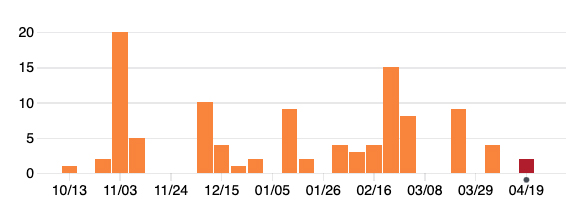
\includegraphics[width=.9\linewidth]{figs/commits.jpg}
  \caption{Commits to the Github repository over the duration of the project.}
  \label{fig:commits}
\end{figure}

For version control, I used Git to track change with a remote repository on GitHub\footnote{https://github.com/}. In total, 104 commits were made over the course of the project as seen in \cref{fig:commits}. My source code is publicly available on GitHub with a README to explain how to use it. The project is licensed under the MIT license, for free modification and reuse while limiting my liability.

The repository served as a backup, allowed me to revert to previous iterations of my code and allowed me to work on multiple computers. In particular, it allowed me to deploy my project to the University's High Performance Computing (HPC) service for running the simulations, as discussed below. In addition, I also performed a hardware backup to an external hard drive twice a week.

\subsection{Development Tools}

I made use of a number of tools to streamline my development process:

\begin{enumerate}

\item I used Travis\footnote{https://travis-ci.org/} for continuous integration. With each commit, a script would automatically run all my unit tests and check my code for correct formatting.
	
\item I used pylint\footnote{https://www.pylint.org/} to lint my code against Google's Python style guide\footnote{http://google.github.io/styleguide/pyguide.html}.
	
\item I used yapf\footnote{https://github.com/google/yapf} to format my code consistently. I implemented a git hook to automatically format my code with each commit; the formatting was further checked by Travis.
	
\end{enumerate}

\section{Summary}\label{section:summary}
% TENSE???
The evolution of language is a challenging problem that can be explored using simulations. In this chapter, I discussed the design of the ``mushroom world'' environment populated by entities controlled by neural networks with a genetic algorithm to model evolution. Three populations can be considered; one without language, one with an external language and one with an evolved language. By comparing these populations in terms of fitness and language production, this simulation can be analysed to determine the parallel ability of the entities to categorise mushrooms and their ability to name them. I concluded the chapter by discussing the professional approach I took to develop, maintain and test my code.

%%%%%%%%%%%%%%%%%%%%%%%%%%%%%%%%%%%%%%%%%%%%%%%%%%%%%%%%%%%%%%%%%%%%%%%
%%%%%%%%%%%%%%%%%%%%%%%%%%%%%%%%%%%%%%%%%%%%%%%%%%%%%%%%%%%%%%%%%%%%%%%
%%%%%%%%%%%%%%%%%%%%%%%%%%%%%%%%%%%%%%%%%%%%%%%%%%%%%%%%%%%%%%%%%%%%%%%
%%%%%%%%%%%%%%%%%%%%%%%%%%%%%%%%%%%%%%%%%%%%%%%%%%%%%%%%%%%%%%%%%%%%%%%
%%%%%%%%%%%%%%%%%%%%%%%%%%%%%%%%%%%%%%%%%%%%%%%%%%%%%%%%%%%%%%%%%%%%%%%
%%%%%%%%%%%%%%%%%%%%%%%%%%%%%%%%%%%%%%%%%%%%%%%%%%%%%%%%%%%%%%%%%%%%%%%
%%%%%%%%%%%%%%%%%%%%%%%%%%%%%%%%%%%%%%%%%%%%%%%%%%%%%%%%%%%%%%%%%%%%%%%
%%%%%%%%%%%%%%%%%%%%%%%%%%%%%%%%%%%%%%%%%%%%%%%%%%%%%%%%%%%%%%%%%%%%%%%
% Implementation

\chapter{Implementation}

% TODO: Maybe cut down on the description of each method and add in some descriptions of the methods in the Simulation class that have been added since

\begin{figure}[t]
  \centering
  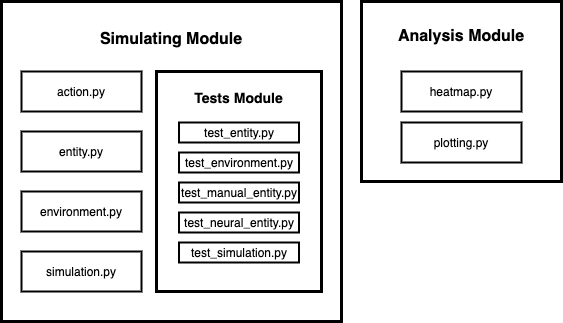
\includegraphics[width=.8\linewidth]{figs/modules}
  \caption{Core modules for my project}
  \label{fig:modules}
\end{figure}

\begin{figure}[p]
  \centering
  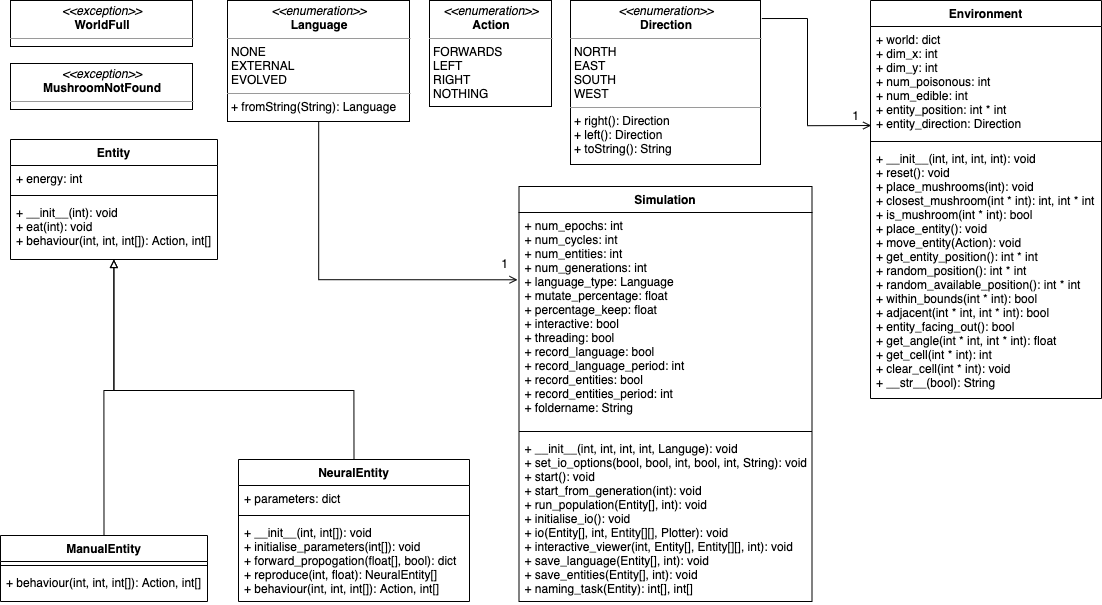
\includegraphics[angle=90, width=.9\linewidth]{figs/uml}
  \caption{UML Diagram for the Simulating Module}
  \label{fig:uml}
\end{figure}

% THIS FIGURE COULD BE LANDSCAPE

\emph{\cref{section:impl-high} of this chapter introduces the modular structure of my implementation. In Sections \ref{section:impl-env} to \ref{section:simulation}, I detail the Environment, Entity and Simulation modules. I discuss my analysis tools in \cref{section:impl-analysis}}.

\section{High-level Overview}\label{section:impl-high}

The implementation of my project is split into three modules as seen in \cref{fig:modules}. The Simulating module contains all the code relevant to creating the simulation. This covers the ``Implementing the Simulation'' requirements for the project described in \cref{section:requirements}. The Analysis module contains functions for plotting different graphs and carrying out the ``Analysis of the Simulation'' requirements for the project.

Within the Simulating module, the classes correspond to the core concepts detailed in Chapter 2. A full UML diagram of this module (excluding tests) can be seen in \cref{fig:uml}. The Entity class and sub-classes correspond to the entities described in \cref{section:entities}. The Environment class corresponds to the ``mushroom world'' simulation environment described in \cref{section:world}. The Simulation class corresponds to the actual simulation, including the genetic algorithm (\S\ref{section:genetic}) and the different populations (\S\ref{section:populations}).

The Analysis module contains the code to analyse the simulation. This includes the plotting of generational fitness, language frequency and quality index as described in \cref{section:analysis}. It also contains another file to produces heatmap plots from the neural networks of a population.

\section{Environment}\label{section:impl-env}

The Environment module contains the Direction enumeration and the Environment class. These are used to represent the state of the mushroom world including the position of the mushrooms and the entity and the direction that the entity is facing. It contains methods for populating the world with mushrooms, managing the state of the world and querying the world, totalling 385 lines of code.

\subsection{Mushrooms}\label{section:mushrooms}

Mushrooms are represented as 10-bit integers. Conceptually, each bit corresponds to a binary property of the mushroom. Poisonous mushrooms are represented as the bit-string \verb!0b1111100000! with one randomly-chosen bit flipped. Similarly, edible mushrooms are represented by the bit-string \verb~0b0000011111~, again with one bit flipped. This means that all mushrooms within a class share the same prototype with some variations to simulate visual inconsistencies. %Using bit-wise arithmetic, I implemented functions to quickly generate mushrooms and test if given mushrooms were edible or poisonous.

\subsection{Representation of the World}\label{section:representation-of-world}

The 20x20 mushroom world is stored as a dictionary, mapping from (x,y) coordinates to mushroom values. Since there are at most 20 mushrooms at any point in the simulation, this dictionary holds a maximum of 20 values at once.

This data structure is chosen over an array representation as the world is sparse. Since the \texttt{closest\_mushroom()} function is called every simulation frame and involves iterating over every mushroom, we want this to be efficient. To compare the two data structures, I ran a benchmark. This benchmark created worlds of both types, populated each with 20 mushrooms and timing how long it took to iterate through all 20 mushrooms. By taking an average of 10000 worlds, I found that the dictionary representation was 14.1 times faster, with an average time of 3.3\textmu s (with a variance of $5.61\times10^-13$) compared to 46.3\textmu s (with a variance of $8.32\times10^-11$) for the array representation. The benchmark script can be found in Appendix~\ref{chapter:benchmark}.

Two run-time exceptions are implemented, \texttt{WorldFull} and \texttt{MushroomNotFound}, thrown when the world is full and empty respectively. Positions in the world are passed between methods as integer pairs (x, y). For clarity, the type \texttt{pos} will be used when such a pair is used.

\subsection{Environment Functionality}

The methods in the Environment module can be split into four groups; world initialisation, utilities, mushroom manipulation and entity manipulation.

{\bf World Initialisation:} An Environment object is created by specifying the dimensions of the world and the number of edible and poisonous mushrooms expected. These are three of the `arbitrary' parameters described in \cref{table:constants}; by default the world is 20x20 and 10 of each mushroom type is placed randomly at the start of each epoch. After creating a new object, the initialisation method calls the \texttt{reset()} method to place the mushrooms, a method separated from the initialisation because the world needs to be reset at the start of each of the epochs.

{\bf Utility Methods:} Seven methods were implemented for managing the state of the world. These included calculating adjacency information, angles between positions, querying individual cells and finding available cells.

{\bf Mushroom Manipulation:} Three methods were implemented for manipulating mushrooms in the world. In particular, the \texttt{closest\_mushroom} method loops through the position keys in the dictionary and for each of these calculate the Manhattan distance. The Manhattan distance is used because it is faster to calculate, it is always an overestimate (or equal to) the Euclidian distance and because the Entity can only move rectilinearly.

{\bf Entity Manipulation:} The world keeps track of the position and direction of the entity within it. This introduces a layer of abstraction between the Entity class and the Environment class; the Entity class is only concerned with the behaviour of the entity independently of the actual representation of its position and movement within the virtual world. The Simulation class acts as an interface between instances of these objects, discussed in \cref{section:simulation}. Five methods in the Environment class are used to move and query the position and direction of the entity, where the direction is stored using the Direction enumeration. In particular, the \texttt{entity\_facing\_out()} method is used for an optimisation discussed in \cref{section:optimisations}.

\subsection{Testing}

Using the \texttt{pytest} library\footnote{\url{https://docs.pytest.org/en/latest}}, I produced a total of 68 unit tests to assert the behaviour of the Environment class. This was done early to ensure that any subsequent refactoring of the code would retain the correct behaviour of the program. Upon discovering bugs during the development process, I produced regression tests to prevent the reemergence of bugs later in development. 

Unit tests were also produced for the Entities and Simulation module, totalling 914 lines of code.

\section{Entities}

The Entities module, totalling 342 lines of code, contains the Entity class and its two subclasses; ManualEntity and NeuralEntity. Separately, the Action module contains the Action enumeration to describe the possible actions taken by the entity; \texttt{FORWARDS} to move once cell forwards, \texttt{LEFT} to turn 90º left, \texttt{RIGHT} to turn 90º right and \texttt{NONE} to do nothing. The full UML diagram can be seen in \cref{fig:uml}.

\subsection{Abstract Specification}

The Entity class acts as an empty parent class. As state, it has an \texttt{fitness} value which is used to determine the fitness of the entity. The \texttt{eat(int)} method changes this value according to equation \ref{equation:fitness}. 

The Entity class also defines the method \texttt{behaviour(float, int, float[]): Action, int[]}. This method describes the expected input-output behaviour of entities discussed in \cref{section:entities}. When passed an angle, a mushroom and an input signal, this method returns an action and an output signal. The angle is passed as a float ranging from 0 to 1. The mushroom's properties are passed as a single integer, as described in \cref{section:mushrooms}. The input and output communication signals are represented by three bits. The outputted action is an instance of the Action enumeration described above. These inputs and outputs are detailed in \cref{table:behaviour}. 

In the Entities class, the \texttt{behaviour} method always returns \texttt{Action.NOTHING} and the vocal signal \texttt{[0,0,0]}.

Note that the inputted and outputted utterances have different data types. All utterances are three-bit strings (encoding 8 possible signals) so outputted signals are always mapped to three bits. However, for the population without language, we input a constant signal \texttt{[0.5, 0.5, 0.5]}, requiring three floats. In the other two populations, the inputted  signals are always comprised of three integer bits.

Before implementing the feed-forward neural networks to control the entities, I created a rule-based entity in the \texttt{ManualEntity} class which extends \texttt{Entity}. It overrides the \texttt{behaviour()} method and implements a simple algorithm to always rotate and move towards the nearest mushroom. On average, this strategy will produce a negative fitness score due to the poisonous mushroom penalty being higher than the edible mushroom reward. This behaviour is not analysed but was useful for the purpose of testing the simulation in the early stages of development due to the deterministic choices made.

\begin{table*}[t]
\centering
 \begin{tabular}{ r | c | c | c}
 \bf{Signal} & \bf{Datatype} & \bf{Description} & \bf{Input / Output} \\ [0.5ex] 
 \hline
location & \texttt{float} & Angle to the nearest mushroom & Input \\
perception & \texttt{int} & Properties of the adjacent mushroom & Input \\
listening & \texttt{float[]} & A 3-bit linguistic signal (heard) & Input \\
vocal & \texttt{int[]} & A 3-bit linguistic signal (spoken) & Output \\
action & \texttt{Action} & The action taken by the Entity & Output \\
\end{tabular}
\caption{Inputs and Outputs of the \texttt{behaviour()} method}
\label{table:behaviour}
\end{table*}

\subsection{Neural Network Entity}

In \cref{section:neural} I gave the general structure for the fully-connected neural network I wanted to use to control the behaviour of the entities. Now that I have defined the datatypes for these inputs and outputs, I can produce a more concrete description of this neural network. 

The neural network has fourteen input units. The first unit is the float value \texttt{location} which describes the angle to the closest mushroom. The next ten units describe the bit-string representation of the mushroom. Note that these values are 0 if the entity is not adjacent to a mushroom (this is controlled by the simulation). The final three units are used for the linguistic input signal. Five hidden units are used, as in \citet{Cangelosi1998}. As discussed in Chapter~2, I implemented the \emph{identity}, \emph{sigmoid} and \emph{ReLU} activation functions.

There are five output units; two of which encode the action taken by the entity (as described above) and the remaining three encode the outputted communication signal (one of eight). The full neural network structure can be seen in \cref{fig:fullneural}.

The \texttt{NeuralEntity} class introduces a few additional methods and state. In particular, two dictionaries store the weights and biases associated with each node in the neural network. Creating a new \texttt{NeuralEntity} calls the \texttt{initialise\_parameters()} method to set the weights and biases to random values chosen from the rectangular distribution over [-1, 1], as specified by \citet{Cangelosi1998}.

The \texttt{forward\_propagation()} method carries out the forward propagation algorithm. The following calculation is made at each layer, where $W_n$ is the weight matrix, $B_n$ is the bias matrix, $f$ is the activation function and $Z_n$ is the resulting activation for layer $n$:

$$ Z_n = f(W_nZ_{n-1} + B_n) $$  

\citet{Cangelosi1998} states that ``for all output units, continuous values are thresholded to either 0 or 1'' but is not clear how this thresholding takes place. I have decided to perform a sigmoid activation on the final layer and rounding the result to return integer values of 0 or 1.

\begin{figure}[t]
  \centering
  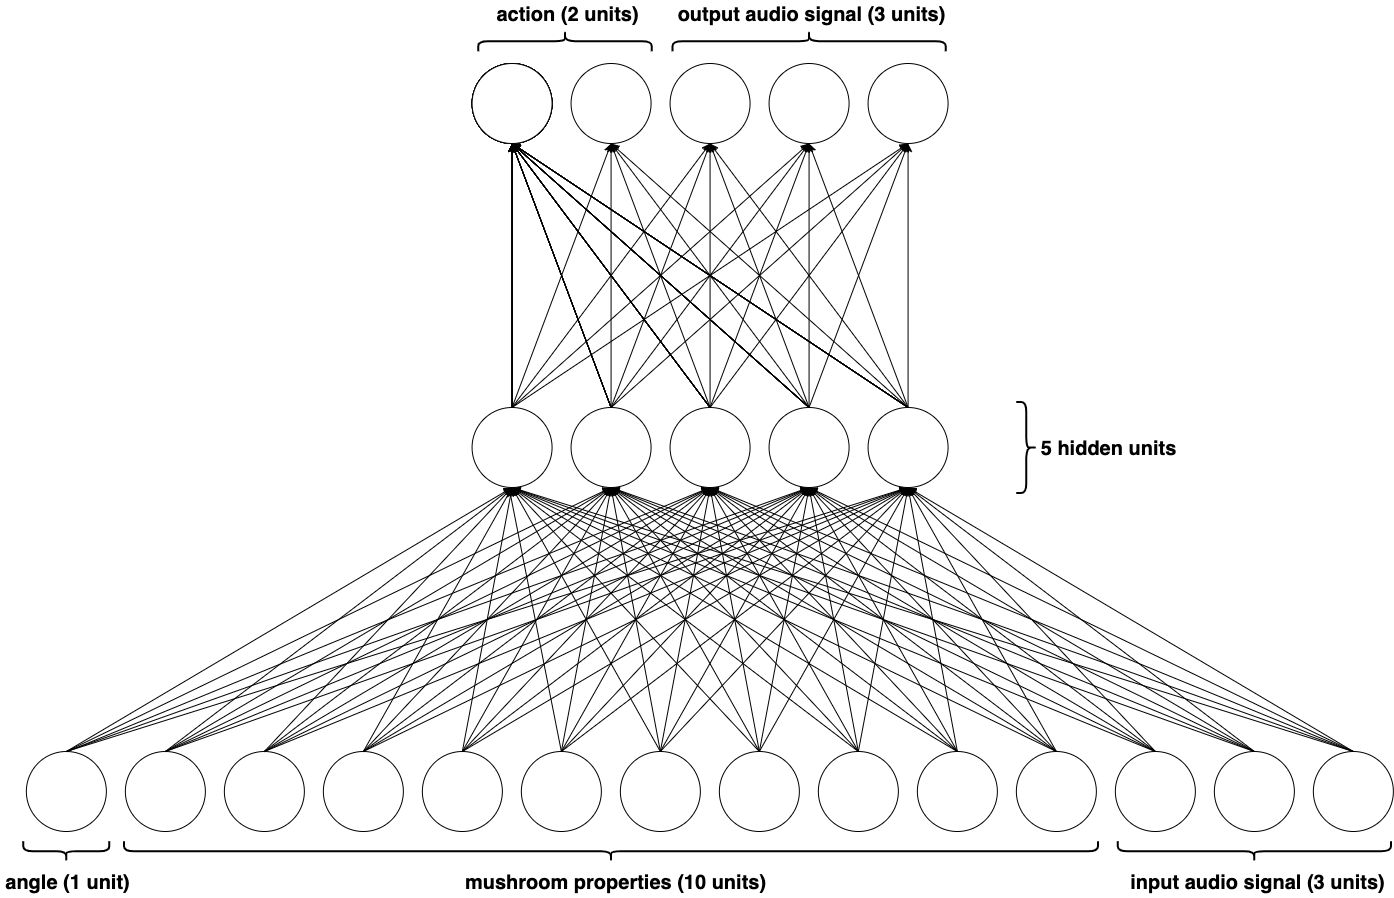
\includegraphics[width=.9\linewidth]{figs/fullneural}
  \caption{Fully-connected ANN to control entity behaviour}
  \label{fig:fullneural}
\end{figure}

% This is the pseudocode for my implementation of forward propagation algorithm:

% %[TODO: MAYBE CUT THIS PSEUDOCODE??]
% \begin{minted}
% [
% frame=lines,
% framesep=2mm,
% baselinestretch=1.2,
% fontsize=\footnotesize,
% linenos
% ]
% {python}
% def forward_propagation(inputs):

%     # Initialise the cache used to store activations and weighted sums
%     activations := []
%     activations[0] := inputs
%     final := number of neural network layers
    
%     # Calculate weighted sum (Z) and activation (A) at each layer
%     for layer in (1, final_layer):
%     	Z := dot(weights[layer], activations[layer-1]) + biases[layer]
%     	activations := activation_function(Z)
    
%     # Calculate activation on the final layer
%     Z := dot(weights[final], activations[final-1]) + biases[final]
%     activations[final] := sigmoid(Z)
    
%     # Round final layer to 0 or 1 and return
%     outputs := round(activations[final], 0, 1)
%     return outputs

% \end{minted}

\texttt{NeuralEntity} overrides \texttt{behaviour()} in order to apply the neural network to the inputs. Given the inputs, it constructs a 14-element float vector as specified in \cref{fig:fullneural}, in particular converting the integer mushroom to an array of bits. It then feeds this input vector to the \texttt{forward\_propagation()} method to get the output vector. The first two bits of this output vector are parsed as an instance of Action and the last three bits are returned as the output signal.

\subsection{Reproduction}

An important aspect of these neural entities is their ability to asexually reproduce, a vital part of the genetic algorithm.

The two parameters specify the number of children, $n$, to produce and the percentage of weights, $p$, in the neural network to mutate. When called, the entity starts by producing $n$ deep copies of itself. For each of these children, it iterates through the weights and biases of their neural networks and uses $p$ to decide whether to mutate it. Mutation occurs by adding a random value in the rectangular distribution specified by [-1, 1] to the current value.

\section{Simulation}\label{section:simulation}

The Simulation module, seen in \cref{fig:uml}, contains the Simulation class and the Language enumeration for implementing the simulation. The Simulation class is responsible for implementing the per-entity simulation (750 cycles in the Environment described above) and the population behaviour, including the genetic algorithm. The Language enumeration describes the differences in language between the populations as described in \cref{section:populations}; \texttt{NONE} is for no language, \texttt{EXTERNAL} for the external language and \texttt{EVOLVED} for the evolved language. Together, these total 685 lines of code.

\subsection{Initialising the Simulation}\label{section:simulation-initialise}

An instance of a Simulation object stores the parameters of the simulation and provides methods that run single-entity simulations and the genetic algorithm. The initialisation method sets the number of epochs, cycles per epoch, population size and the number of generations to run the simulation for as outlined in \cref{section:world}.

Further specified are two parameters used by the genetic algorithm; the percentage of the population chosen to reproduce (20\% by default) and the percentage of weights to mutate (10\% by default). These were discussed in \cref{section:genetic} and are listed with the other simulation parameters in \cref{table:constants}.

\subsection{Single-Entity Simulation Run}\label{section:single-implementation}

The \texttt{run\_single()} method performs the main simulation for each entity. The pseudocode for this function is shown below. Taking a single entity as a parameter, it performs the relevant operations required to allow the entity to `live' in an instance of the Environment class for \texttt{num\_epochs} of \texttt{num\_cycles} time steps each. During this time, the entity's \texttt{behaviour()} method is passed the appropriate inputs according to its current position in the environment (lines 14 to 19). The outputs of the \texttt{behaviour()} method are interpreted accordingly, moving the entity in the environment (line 20). When the entity shares a cell with a mushroom, it eats it, changing its fitness score accordingly and the mushroom is removed from the environment (lines 23 to 25).

\begin{minted}
[
frame=lines,
framesep=2mm,
baselinestretch=1.2,
fontsize=\footnotesize,
linenos
]
{python}
def run_single(entity):

	# Create a random environment
	env := new Environment
  
	for epoch in num_epochs:

    	# Reset mushroom positions and entity position between each epoch
    	env.reset()
    	env.place_entity()
    
    	for cycle in num_cycles:
    		# Gather inputs for the entity
    		location := angle from entity to closest mushroom
    		perception := bit string of mushroom if entity adjacent to it
    		listening := input signal according to language type
        
    		# Get behaviour of the entity and move accordingly
    		action := entity.behaviour(location, perception, listening)
    		env.move_entity(action)
          
    		# Entity eats a mushroom if on top of one
    		if env.entity_position is a mushroom:
    			entity.eat(mushroom)
    			env.remove(mushroom)

\end{minted}

Line 16 is implemented as three cases according to the \texttt{language\_type} property of the simulation. For no language, the signal is just set to \texttt{[0.5, 0.5, 0.5]}. For the external language, this signal is set to \texttt{[1, 0, 0]} if the closest mushroom is edible and \texttt{[0, 1, 0]} if it is poisonous.

For the evolved language, this step is slightly more complicated. The \texttt{run\_single()} method is also passed an array of the 99 other entities in the population and at each simulation step, one of these is randomly chosen to be the `partner entity' to name the closest mushroom for the primary entity. This other entity is given the same \texttt{location} parameter and a constant value of \texttt{[0.5, 0.5, 0.5]} as its \texttt{listening} signal but always receives the properties of the mushroom as its \texttt{perception} input, regardless of distance to the mushroom. The \texttt{action} output of the call to this partner entity's \texttt{behaviour()} call is ignored but the outputted signal is used as the inputted \texttt{listening} signal for our primary entity.

\subsection{Genetic Algorithm}

The \texttt{run\_population()} method implements the genetic algorithm used for this simulation. Given an initial population of entities, it runs the algorithm for \texttt{num\_generations} generations. The algorithm has three steps; performing the \texttt{run\_single()} method for each entity of the population, sorting the population to find the entities with the highest fitness and finally choosing a certain percentage of the fittest entities to reproduce to create the next population. The pseudocode for this process is shown below.

Lines 7-9 perform this first step by running the simulation for each entity in the current population. This simulation will update the fitness of each entity each time that an entity eats a mushroom. If the language being used is the evolved language, the \texttt{run\_single()} method is also passed a list of the other entities in the population to perform the appropriate naming as discussed in \cref{section:single-implementation}.

Lines 12-13 perform the second step by simply sorting the list of entities according to the fitness achieved in each simulation. The top percentage of these entities is then selected for reproduction.

Lines 16-19 create the next population by calling the \texttt{reproduce()} method on each of the fittest parent entities identified. This method is passed the number of children to produce (the reciprocal of the percentage of parents selected) and the percentage of weights to adjust in the mutation process.

\begin{minted}
[
frame=lines,
framesep=2mm,
baselinestretch=1.2,
fontsize=\footnotesize,
linenos
]
{python}

def run_population(entities):

	for generation in num_generations:

    	# Step 1: Run the simulation for each entity
    	# Pass the remaining population for the evolved language
    	for entity in entities:
    		population := entities - {entity}
    		run_single(entity, population)
               
    	# Step 2: Sort the entities by their fitness and select the best
    	sort(entities, entity.fitness)
    	best_entities := top percentage_keep of entities
    
    	# Step 3: Create a new population from the fittest entities
    	children := []
    	for entity in best_entities:
    		children += entity.reproduce(1/percentage_keep, mutate_percentage)
    	population := children

\end{minted}

Two key constants in this algorithm are \texttt{mutate\_percentage} and \texttt{percentage\_keep} which set the percentage of weights to mutate and the percentage of the population chosen for reproduction respectively. The setting of these constants was discussed in \cref{section:simulation-initialise}.

\subsection{Running the Simulations Using HPC}\label{section:running}

To run experiments, I acquired access to the University of Cambridge's High Performance Computing (HPC) facility. This gave me access to an environment where I could set up experiments and schedule runs of my program using the SLURM workload manager\footnote{\url{https://slurm.schedmd.com/}}. I created a series of bash scripts that would allow me to schedule a batch of jobs at once (for example 10 independent runs of the genetic algorithm for each language type). I used the \texttt{rsync} command to copy computed data to my local file system. This work cycle allowed me to work quickly and effectively, all while avoiding having to use my own laptop for computationally demanding jobs. 

To further speed up running experiments, I used the \texttt{argparse} library to create a command-line interface for my system. This allowed me to run the genetic algorithm, a single-entity simulation or load a previously run simulation from the command line and set any of the simulation and I/O parameters specified in Tables \ref{table:constants} and \ref{table:io-params}. Examples of running my system from the command line can be seen in Appendix~\ref{chapter:simulation-interactivity}.

\subsection{Optimisations}\label{section:optimisations}

Having finished the core implementation of the project early, I implemented optimisations to increase the rate at which I could run experiments. Throughout implementation I made decisions that would favour a faster runtime, such as using \verb|numpy| arrays for matrix operations or using the dictionary-world representation, as discussed in \cref{section:representation-of-world}.

Considering a run of the genetic algorithm informs us that the \texttt{run\_single()} method is called 200000 times when operating on a population of 100 entities for 2000 generations. Each call to this method involves 15 epochs of 50 cycles, or 750 iterations of the perception-action loop described in \cref{section:single-implementation}. Giving us a total of 150 million total iterations, this is a good site for optimisation.

The most expensive operation in this loop is the call to \texttt{behaviour()} which performs forward propagation, involving matrix multiplications. The other operations are less expensive, involving simple variable manipulation. Furthermore, the \texttt{behaviour()} method is called twice for the population with the evolved language (once for the speaker and once for the listener). The average runtimes for the {\bf no language} and {\bf evolved language} populations are 108 minutes and 180 minutes respectively, calculated by comparing the average runtime of ten runs of the genetic algorithm for 1000 generations. We can therefore estimate that calls to the the \texttt{behaviour()} method are responsible for approximately 67\% of the runtime for when the language type is \texttt{NONE} and 80\% when the language type is \texttt{EVOLVED}. My optimisations were thus focused around this call.

{\bf Parallelisation:} The first optimisation was made by taking advantage of the fact that the 100 calls to \texttt{run\_single()} are large (750 simulation cycles each) and do not interact (each entity exists in its own world). These calls are thus \emph{embarrassingly parallel} and so are worthy of parallelisation \citep{mycroft2019}.

Using the \texttt{multiprocessing} library\footnote{\url{https://docs.python.org/3.8/library/multiprocessing.html}}, I replaced the for loop with a \texttt{Pool} object which represents a pool of worker processes. The size of this pool is automatically set according to the number of hardware threads available. Using the \texttt{Pool}, I call the \texttt{starmap} method to dynamically offload the 100 calls to \texttt{run\_single()} to these processes. On my laptop, with 8 hardware threads available, this gave a speedup of $3.96\times$ when running the simulation for 100 generations, averaged over 10 runs. When running my program on the HPC I found that this optimisation was not as effective: although I could allocate 32 hardware threads, a speedup of only $1.06\times$ was achieved, likely due to hidden communication costs between cores not present on my laptop. Allocating this many threads also increased my expenditure so I decided not to use this optimisation when running my experiments.

{\bf Epoch skipping:} By noting that (1) the \texttt{behaviour()} method is deterministic and (2) that the environment is static (besides the entity), I was able to reduce the number of simulation loops required in the \texttt{run\_single()} method. If at any stage the call to \texttt{behaviour()} returns the \texttt{NOTHING} action then due to these two properties, it will continue to do so for the rest of the epoch. Thus, we can simply skip the remainder of the current epoch; the ``Skip None'' optimisation. 

A similar optimisation can be made when the entity attempts to move \texttt{FORWARD} through the edge of the world. The response to this behaviour was not defined in \citet{Cangelosi1998} so I had the entity remain in the same position. This is arbitrary, and I explore alternative choices in \cref{section:simulation-parameters}. As the entity remains in the same position, it will return the same response in the next cycle so we can again skip the epoch. This is the ``Skip Edge'' optimisation. Similar epoch-skipping optimisations can also be considered; such as the ``Detect Looping'' optimisation which determines if the entity is stuck spinning on the spot in either direction by examining the last four actions. 
%Note that in all three of these cases we cannot skip the entire simulation because at the end of each epoch the position of the mushrooms and the entity are reset, which may change the inputs to the function. 

\begin{figure}[t]
  \centering
  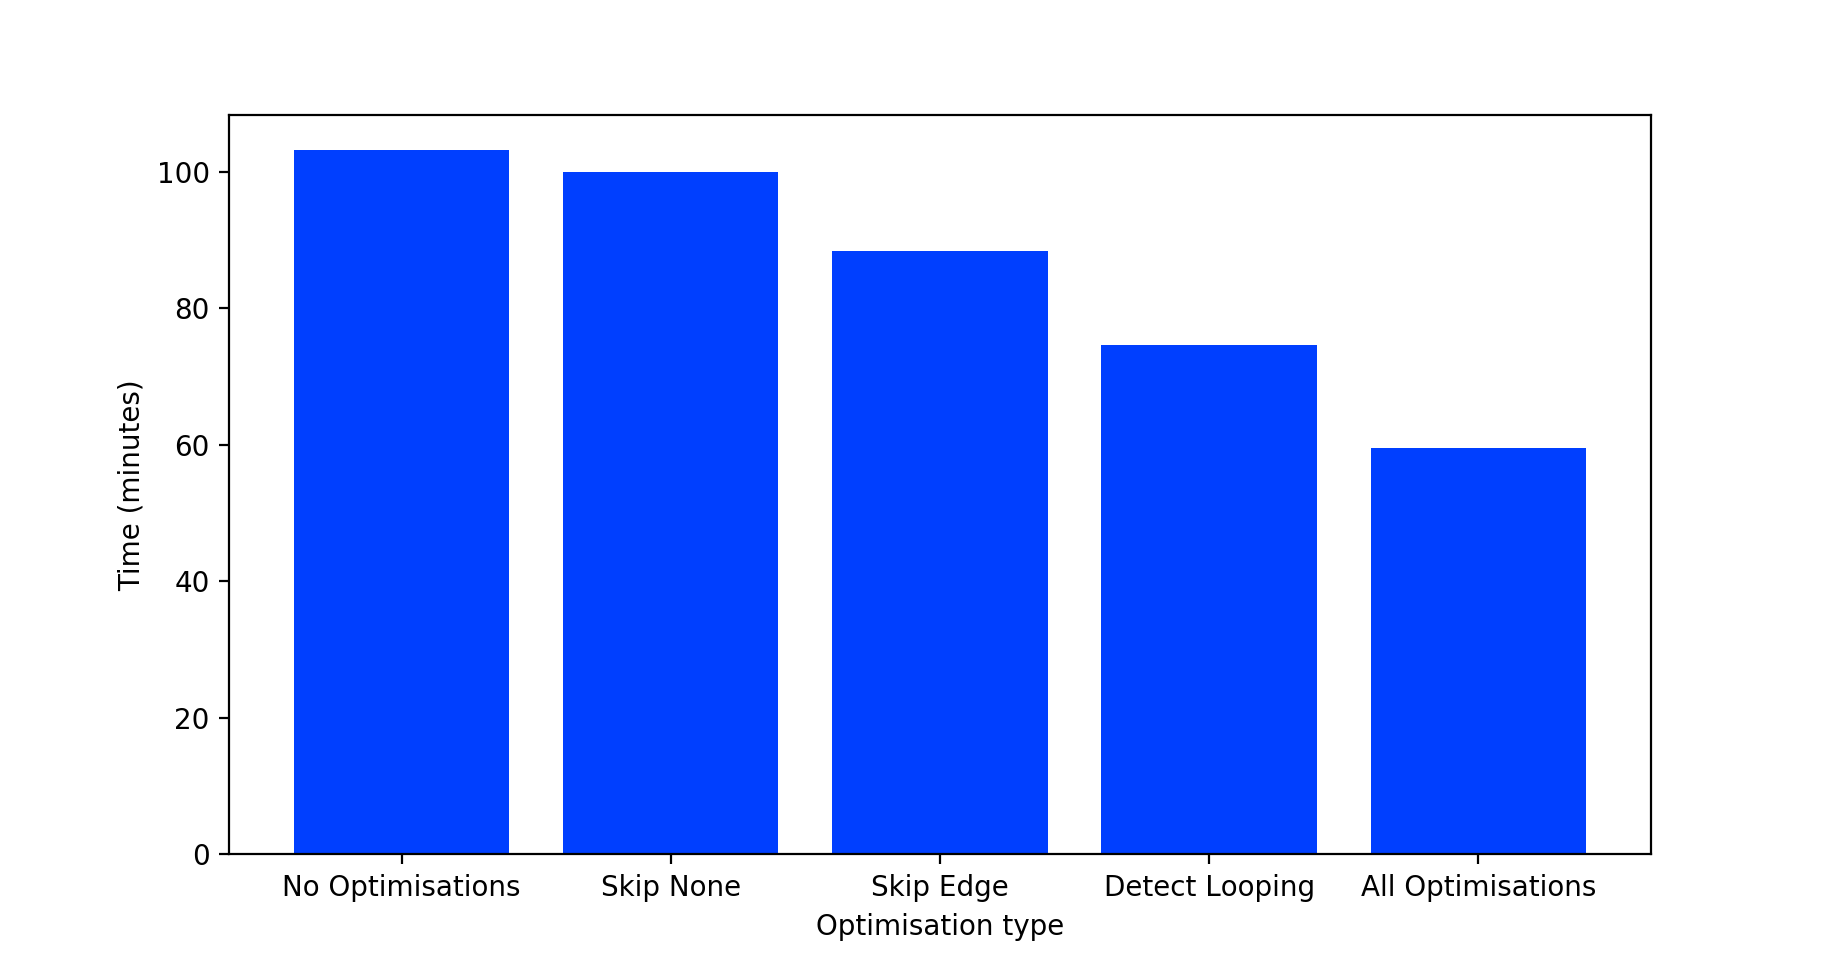
\includegraphics[width=.9\linewidth]{figs/speedup}
  \caption{Time taken to run 1000 generations of the genetic algorithm on a population with no language for each optimisation, averaged over ten runs.}
  \label{fig:speedup}
\end{figure}

\begin{figure}[t]
  \centering
  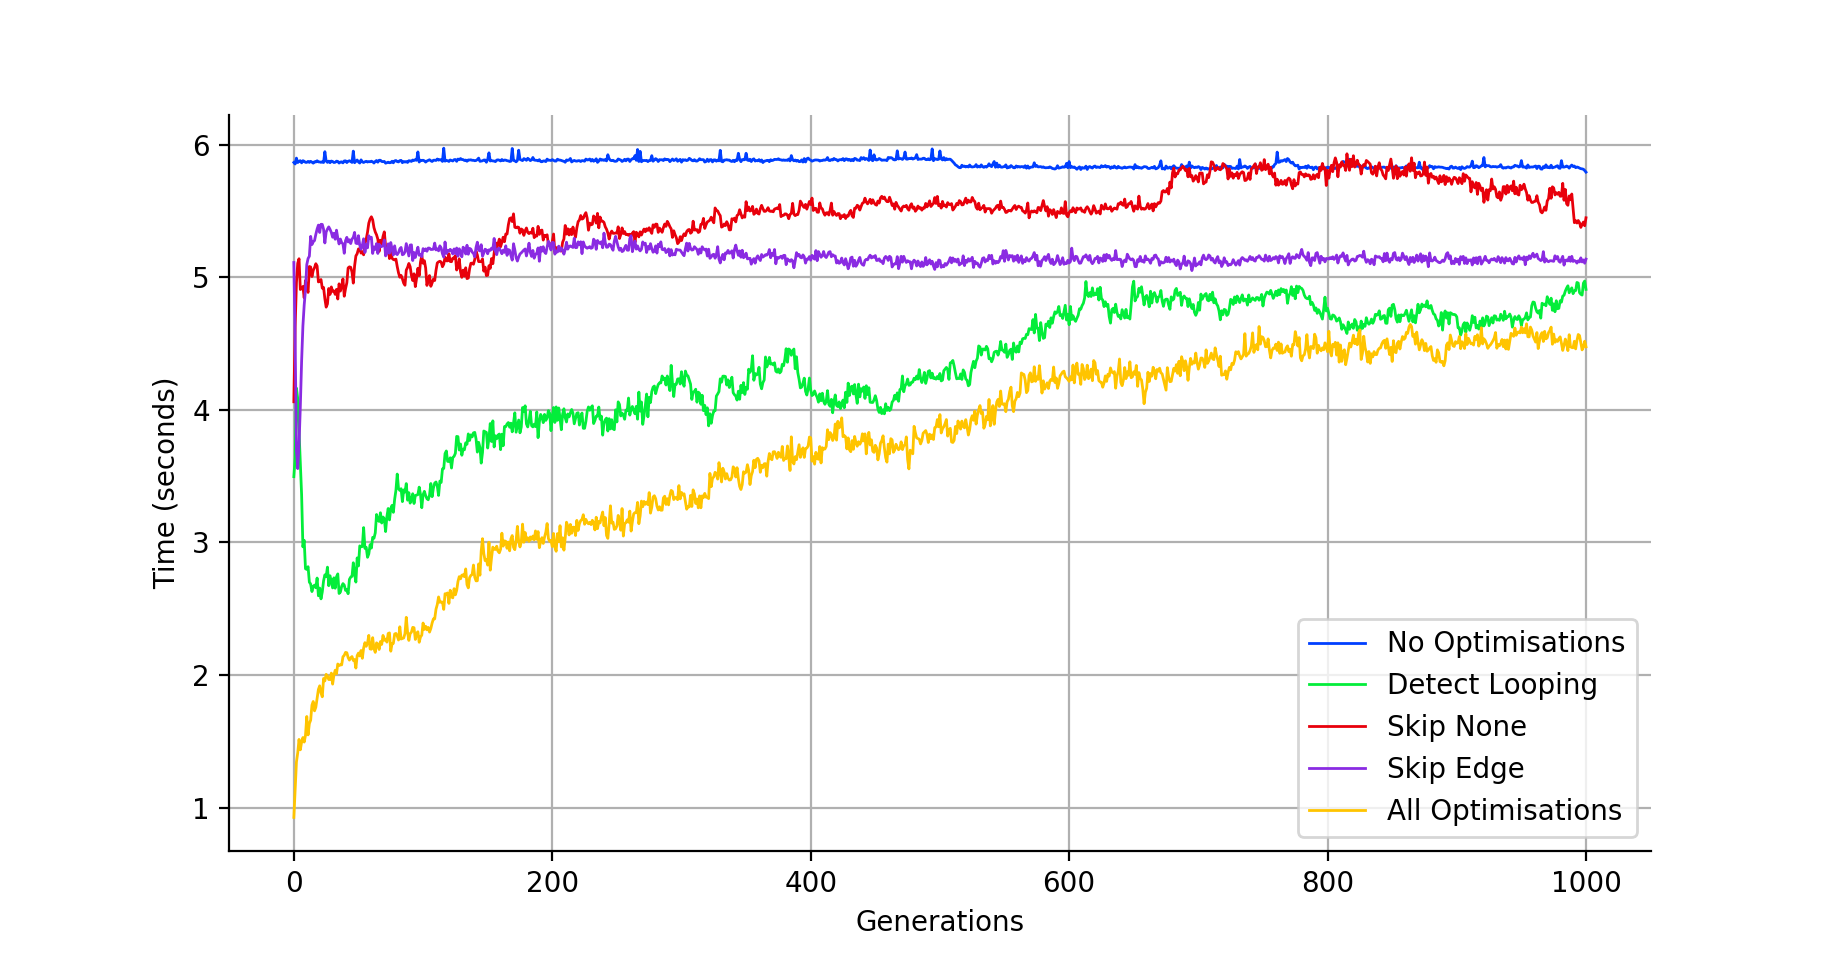
\includegraphics[width=.9\linewidth]{figs/generation-time}
  \caption{Time taken to run each generation of the genetic algorithm on a population with no language for each optimisation, averaged over ten runs.}
  \label{fig:generation-time}
\end{figure}

\cref{fig:speedup} shows how each epoch-skipping optimisation decreases the average runtime of the genetic algorithm. The ``Skip None'', ``Skip Edge'' and ``Detect Looping'' optimisations give speedups of $1.03\times$, $1.17\times$ and $1.38\times$ respectively. When all three of these optimisations are used, there is a total speedup of $1.78\times$, significantly reducing the time taken to run experiments.

%Further epoch-skipping optimisations could be implemented by detecting more complicated multi-cycle looping behaviours but these would give diminishing returns. This can be seen in the difference between the "Detecting Looping" optimisation and the "Skip None" optimisation; more complicated behaviours occur less frequently, cost more to detect and offer less of a speedup as fewer cycles would be skipped. 

It is worth noting that \emph{by the nature of the genetic algorithm, the population will learn to avoid the very behaviours that lend themselves to optimisations}. This can be seen in the time taken to simulate each generation; in \cref{fig:generation-time} we can see that ``Skip None'' optimisation is very effective in early generations but gradually has less effect. The population learns to avoid producing a \texttt{NONE} action, as this wastes previous time that could be spent searching for mushrooms. A similar effect is seen for the ``Detect Looping'' optimisation but the inverse is seen for the ``Skip Edge'' optimisation; the entities do not know where the edge of the world is and so this behaviour occurs more frequently as the entities learn to explore.

\subsection{Interactivity}\label{section:interactivity}

During development, I implemented interactive behaviour to allow me to watch the simulation and genetic algorithm occur step-by-step. This was also useful for evaluation as it allowed me to analyse the behaviour of each population by replaying saved simulations from different generations. This behaviour is activated using a `\texttt{-i}' flag in the command-line interface.

Enabling this behaviour produces an average fitness graph, updated continuously with the latest average fitness of the population. Running the simulation in this interactive mode also displays useful information at each generation and even allows the user to watch the behaviour of a single entity in a visual representation of the \texttt{Environment} object. Examples and descriptions of the live graph, generational information and single-simulation interactivity can be found in Appendix~\ref{chapter:simulation-interactivity}.

% MISSING FIGURE HERE

% CUT: The \texttt{io()} function also outputs other useful information and pauses the genetic algorithm to allow for interactivity. At each generation, the current generation, current list of fitness values and average energy for the current population is printed. The program then waits for user input before continuing. An inputted number will run the genetic algorithm for that many generations. Alternatively, by entering ``watch'' followed by a number, the program will allow the user to watch the behaviour of the entity indexed by the inputted number within the simulation. This is calls \texttt{run\_single()} again on the selected entity with an additional parameter, \texttt{viewer}, set to True.

% ALSO CUT: The \texttt{run\_single()} method also has optional interactive behaviour. At each simulation step, the current world is displayed as a grid with emojis used to indicate the positions of edible and poisonous mushrooms. The position and direction of the entity is indicated using a triangle. This is done by converting the \texttt{Environment} object to a string; I had provided an implementation of the \texttt{\_\_str\_\_} method in the Environment class. Further information is also displayed, such as the current inputs and outputs to the entity at each step. This method is also paused for interactivity, the user presses ENTER to move to the next step or ESC to leave the viewer. This interactivity was crucial in early testing to locate complicated bugs and perform behavioural tests of the simulation.

\subsection{Data Recording}

For the analysis of the simulation, I implemented a few utility methods to collect data as it ran. The command-line interface is used to set a group of I/O parameters to control the storage of fitness, language and population data. The parameters control whether, where and how frequently this data is stored.% These parameters are detailed in \cref{table:io-params}.

% \begin{table*}[t]
% \centering
%  \begin{tabular}{ c | c | c}
%  \bf{I/O Parameter} & \bf{Description} & \bf{Default Value} \\ [0.5ex] 
%  \hline
% interactive & Sets interactive behaviour on & False \\
% record\_language & Whether to save the language & True \\
% record\_language\_period & How often the language is saved & 1 \\
% record\_entities & Whether to save the population of entities & True \\
% record\_entities\_period & How often the population is saved & 1 \\
% record\_fitness & Whether to save the average fitness & True \\
% foldername & Where the data is saved in the local filesystem & ``folder'' \\
% \end{tabular}
% \caption{Parameters used for controlling the Input and Output of the system}
% \label{table:io-params}
% \end{table*}

By default, at each generation this method records the the average fitness, the language and the neural networks of the population. The language is saved as a frequency table, calculated by calling the \texttt{naming\_task()} method for each entity in the population, which calls \texttt{behaviour()} for 80 different possible inputs and returns the outputted signals. The neural networks are saved in a binary file, used to load previously-run simulations and to analyse the weights and biases of the population.

\section{Simulation Analysis}\label{section:impl-analysis}

The Analysis module seen in \cref{fig:modules} contains the Plotting class and a variety of methods to analyse the simulation in the same manner as \citet{Cangelosi1998}. The Plotting class is used for displaying a live fitness graph, discussed above in \cref{section:interactivity}. A command-line interface was also implemented for this module, allowing me to easily generate different fitness graphs and language frequency distribution graphs as seen in Chapter~4.

\subsection{QI Score}

A particular set of methods were used to calculate the QI score of the language produced by the population as given in equation \ref{equation:qi} in \cref{section:efficiency}. \citet{Cangelosi1998} used this equation to correlate language efficiency with fitness and found that even in a population that did not use language, there was a high correlation between fitness and QI score over 1000 generations. Upon initial analysis of my simulation however, I only achieved low and negative correlation scores between fitness and the QI score defined by equation \ref{equation:qi}, as seen in \cref{table:qi-correlation}.

\begin{table*}[t]
\centering
 \begin{tabular}{ c || c | c | c | c | c}
 \bf{Replication} & \bf{1} & \bf{2} & \bf{3} & \bf{4} & \bf{5}\\
 \hline
  \hline
\bf {QI Equation A} & 0.28 & 0.27 & 0.13 & 0.21 & 0.17 \\
 \hline
\bf {QI Equation B} & 0.54 & 0.69 & 0.41 & 0.57 & 0.52 \\
\end{tabular}
\caption{Correlation of QI Score with Average Fitness for five replications of the simulation. {\bf QI Equation A} is equation \ref{equation:qi} and {\bf QI Equation B} is equation \ref{equation:qibetter}.}
\label{table:qi-correlation}
\end{table*}

Reviewing this equation further we can see that this equation does not match Cangelosi and Parisi's  definition of a productive language. The first half of the equation, $\sum^{8}_{i = 1} |x_i - y_i|$ has a maximum value of 2 if no signal is used for both edible and poisonous mushrooms, so is large if the language is efficient. The second half of this equation, $\min (d_{\mathrm{poisonous}}, d_{\mathrm{edible}})$, has a maximum value of 1.75 if only one signal is used for each mushroom type, thus is also large if the language is efficient. 

This means that if the QI equation is meant to capture language efficiency, these two values should be \emph{added} instead of subtracted. I thus implemented the following equation:

\begin{equation}
\label{equation:qibetter}
\mathrm{QI} = \sum^{8}_{i = 1} |x_i - y_i| + k \times \min (d_{\mathrm{poisonous}}, d_{\mathrm{edible}})
\end{equation}

As well as having logical justification, the preliminary results in \cref{table:qi-correlation} show that this equation produces a better correlation with average fitness than equation \ref{equation:qi}. From this I assume that there was a printing mistake in the published equation that Cangelosi and Parisi gave. 

\section{Summary}

In this chapter I covered my implementation of the ``mushroom world'' simulation. I described the Environment, Entity and Simulation classes and gave details of how I implemented the genetic algorithm and the simulation loop. I discussed my testing framework, how I made the simulation interactive and how I recorded data for analysing the simulation. Through careful analysis, I was able to produce key optimisations for my simulation and also discover a printing error published in \citet{Cangelosi1998}.

%%%%%%%%%%%%%%%%%%%%%%%%%%%%%%%%%%%%%%%%%%%%%%%%%%%%%%%%%%%%%%%%%%%%%%%
%%%%%%%%%%%%%%%%%%%%%%%%%%%%%%%%%%%%%%%%%%%%%%%%%%%%%%%%%%%%%%%%%%%%%%%
%%%%%%%%%%%%%%%%%%%%%%%%%%%%%%%%%%%%%%%%%%%%%%%%%%%%%%%%%%%%%%%%%%%%%%%
%%%%%%%%%%%%%%%%%%%%%%%%%%%%%%%%%%%%%%%%%%%%%%%%%%%%%%%%%%%%%%%%%%%%%%%
%%%%%%%%%%%%%%%%%%%%%%%%%%%%%%%%%%%%%%%%%%%%%%%%%%%%%%%%%%%%%%%%%%%%%%%
%%%%%%%%%%%%%%%%%%%%%%%%%%%%%%%%%%%%%%%%%%%%%%%%%%%%%%%%%%%%%%%%%%%%%%%
%%%%%%%%%%%%%%%%%%%%%%%%%%%%%%%%%%%%%%%%%%%%%%%%%%%%%%%%%%%%%%%%%%%%%%%
%%%%%%%%%%%%%%%%%%%%%%%%%%%%%%%%%%%%%%%%%%%%%%%%%%%%%%%%%%%%%%%%%%%%%%%
% Evaluation

\chapter{Evaluation}

\emph{In \cref{section:popfit}, I begin by examining the average fitness of different populations with default simulation parameters. In \cref{section:languageanalysis} I then examine the language produced by the evolved language population and investigate the QI of this language. }

\emph{In \cref{section:behaviouranalysis}, I conduct my own, deeper analysis of the simulation by examining the convergence of the neural networks to different behavioural states. Finally I explore the robustness of the simulation to the choice of simulation parameters in \cref{section:simulation-parameters}, and discuss whether the conclusions of \citet{Cangelosi1998} still hold.}

\section{Initial Analysis}

\subsection{Population Fitness}\label{section:popfit}
 
The first analysis that we can conduct is how the average fitness of each population compares across many iterations of the genetic algorithm.

\citet{Cangelosi1998} performed this experiment by running the simulation 5 times for each language type for 1000 generations. They chose to stop the simulation at 1000 generations because by this point all three populations were capable of discriminating between the two mushroom types and had further learnt the correct behaviour (avoiding the poisonous and eating the edible ones). The result of their experiment can be seen in \cref{fig:cangelosi-results}.

In my analysis I chose to run each experiment for 2000 generations and average across 10 replications for each population type. The choice of 2000 generations was made to explore potential behaviour that \citet{Cangelosi1998} may have missed and the choice of 10 runs was made to increase the statistical validity of my results due to high variance observed between runs. I was also able to run these experiments due to my access to the HPC facility; computing power that \citet{Cangelosi1998} may not have had. 

\begin{figure*}[t]
   \centering
   \begin{minipage}{0.49\textwidth}
          \centering
          \captionsetup{width=.9\linewidth}
          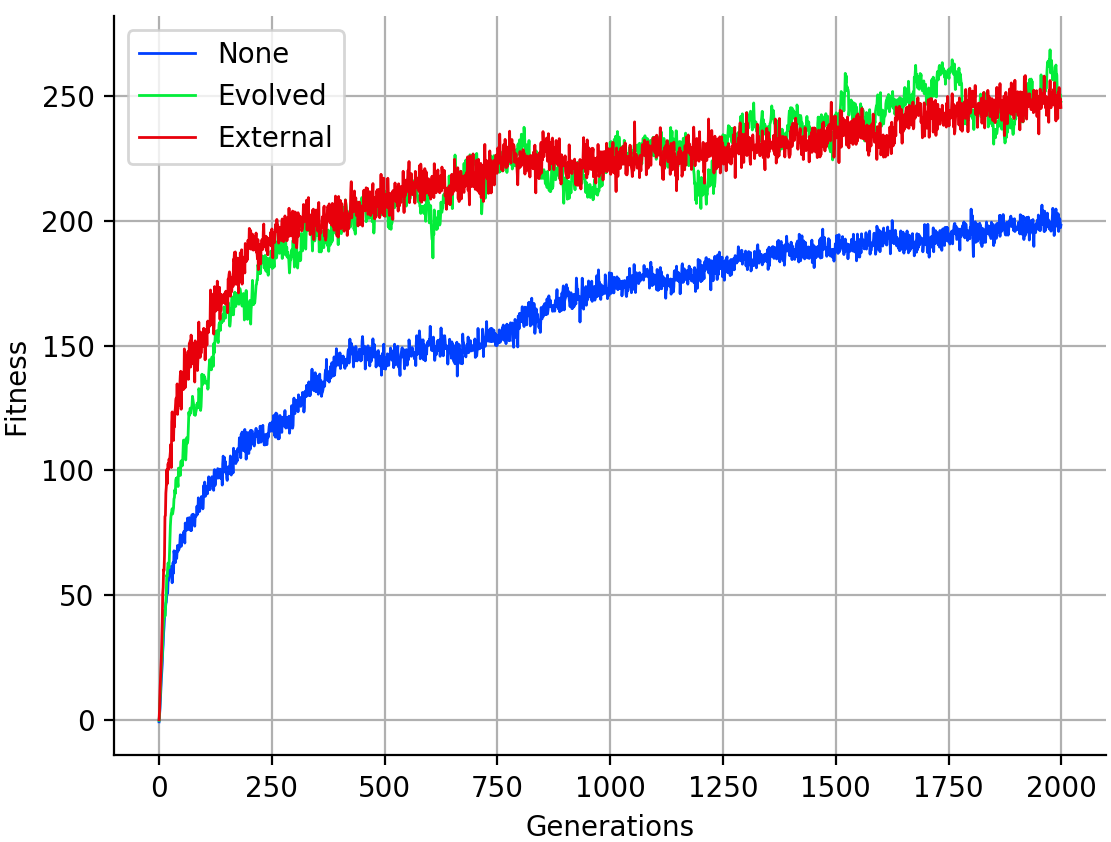
\includegraphics[width=1.\linewidth]{results/average-relu.png}
          \caption{Average fitness of each population, averaged over 10 replications, with a {\bf ReLU} hidden layer activation.}
          \label{fig:average-relu}
   \end{minipage}
   \begin{minipage}{0.49\textwidth}
          \centering
          \captionsetup{width=.9\linewidth}
          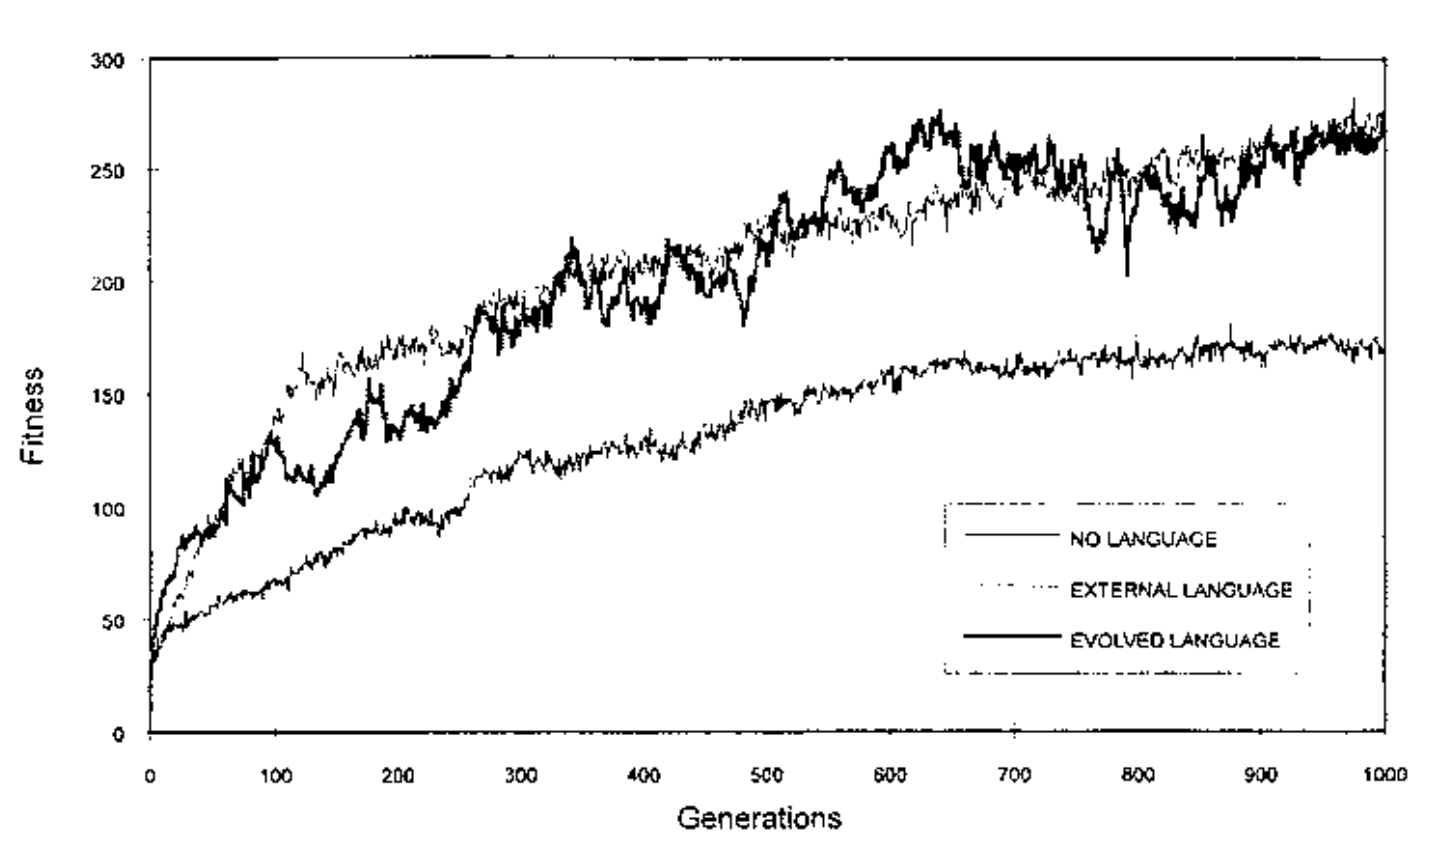
\includegraphics[width=1.\linewidth]{figs/fitness.png}
          \caption{Average fitness of each population, averaged over 5 replications. Source: \citet{Cangelosi1998}.}
          \label{fig:cangelosi-results}
   \end{minipage}
\end{figure*}

The first result of this experiment can be seen in \cref{fig:average-relu}. The simulation parameters used were the defaults detailed in \cref{table:constants}, with the ReLU activation function used in the hidden layer of the neural networks and a sigmoid activation function used at the final layer. Unless otherwise specified, these parameters will be assumed for the rest of this chapter.

From this experiment we can conclude that language is a useful adaptation for our entities. The population with {\bf no language} achieves an average fitness of 200 by the end of the 2000 generations whereas the two populations with language achieve an average fitness of 250 by generation 2000. A behavioural test shows that entities in these population use the signals provided to move away from poisonous mushrooms regardless of distance and approach edible mushrooms to eat; the population without language must approach each mushroom in order to categorise them and behave accordingly. This takes additional simulation cycles, explaining the lower fitness achieved.

\begin{figure*}[t]
   \centering
   \begin{minipage}{0.49\textwidth}
          \centering
          \captionsetup{width=.9\linewidth}
          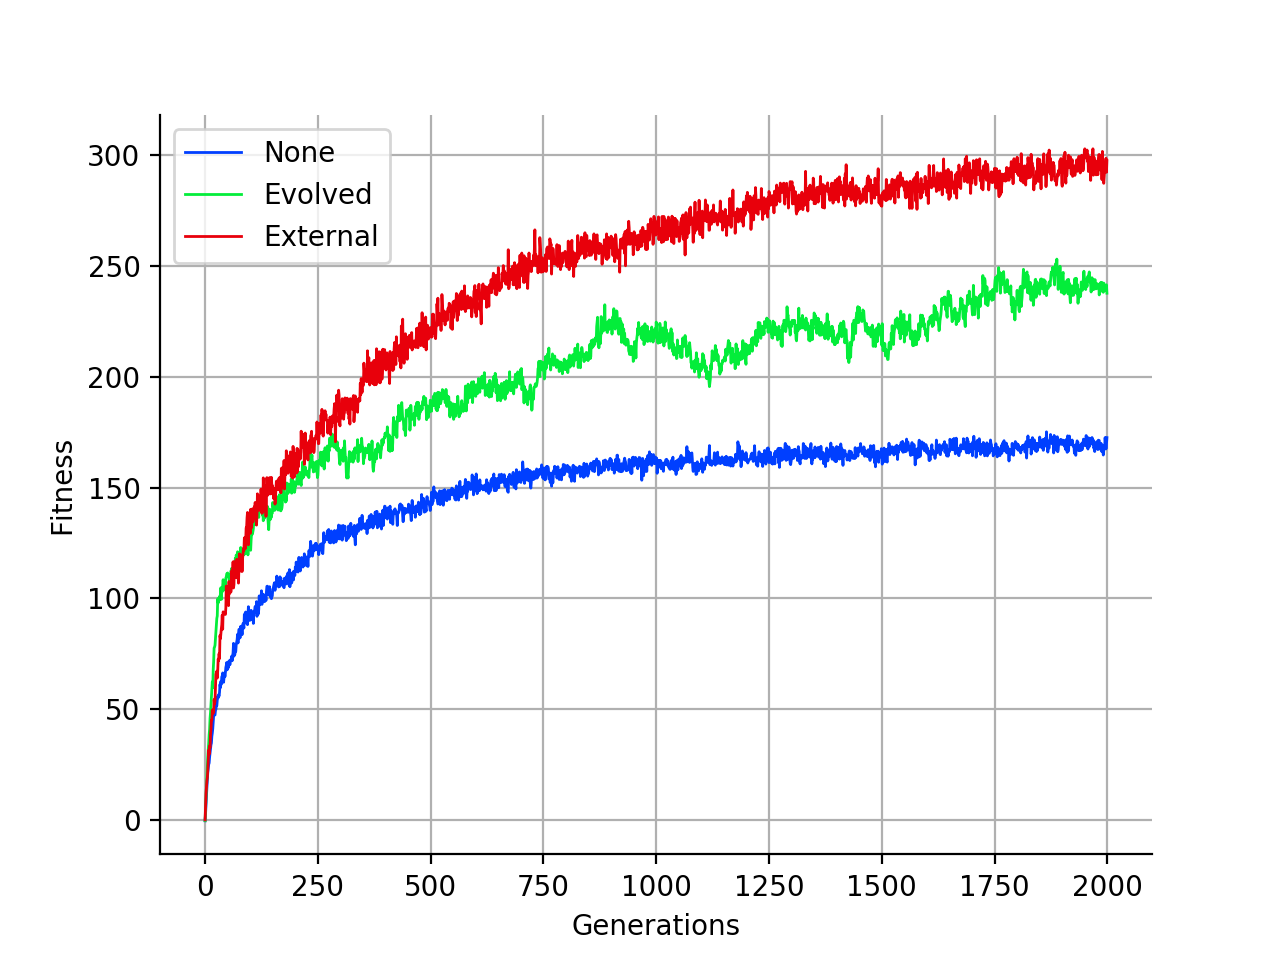
\includegraphics[width=1.\linewidth]{results/average-identity.png}
          \caption{Average fitness of each population, averaged over 10 replications, with an {\bf identity} hidden layer activation.}
          \label{fig:average-identity}
   \end{minipage}
   \begin{minipage}{0.49\textwidth}
          \centering
          \captionsetup{width=.9\linewidth}
          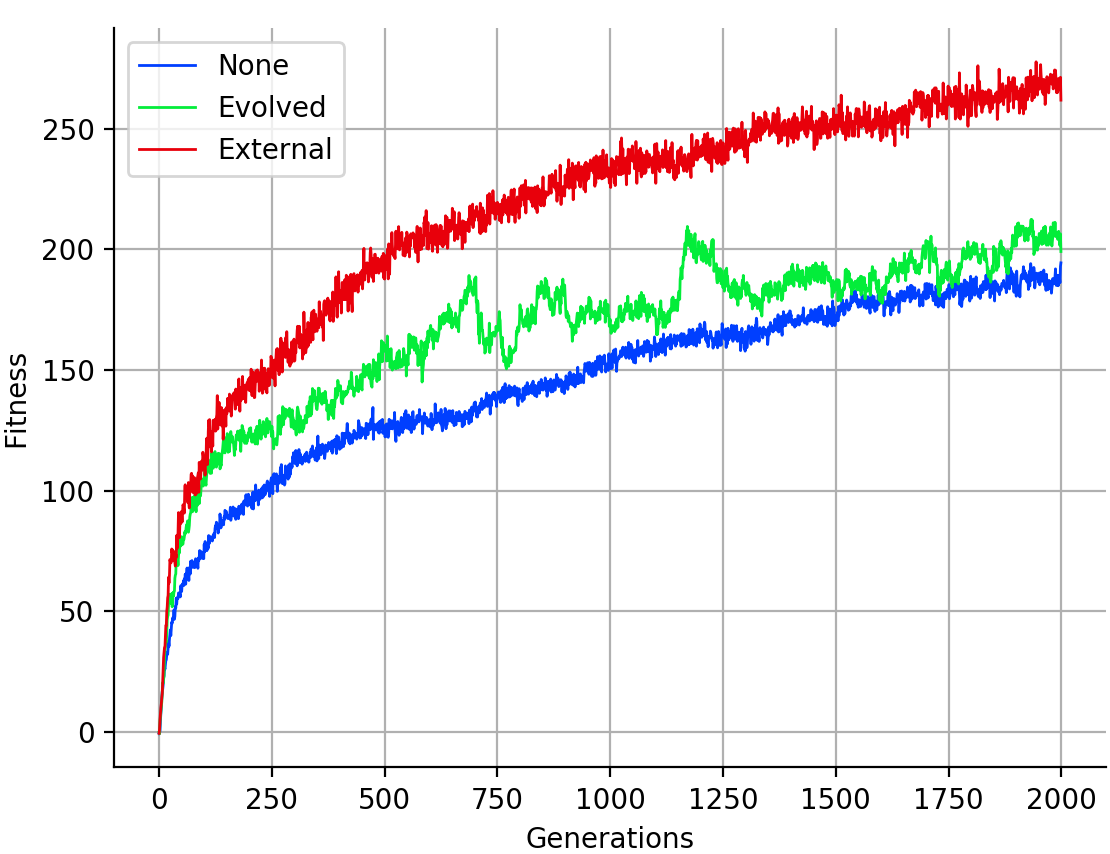
\includegraphics[width=1.\linewidth]{results/average-sigmoid.png}
          \caption{Average fitness of each population, averaged over 10 replications, with a {\bf sigmoid} hidden layer activation.}
          \label{fig:average-sigmoid}
   \end{minipage}
\end{figure*}

As can be seen by \cref{fig:cangelosi-results}, these were the same conclusions reached by \citet{Cangelosi1998}. However, they didn't specify which activation functions were used in their implementation. In \cref{fig:average-identity} and \ref{fig:average-sigmoid} we can see the results of the same experiment repeated using the identity activation function and sigmoid activation function respectively, with no other parameters changed. We see similar results as when using the ReLU activation function but with slight differences. For the case of the identity function, the {\bf evolved language} populations perform the same as with ReLU but the {\bf external language} populations perform better and the {\bf no language} populations perform worse. With the sigmoid activation function the results are very similar to with ReLU except that the {\bf evolved language} performance is closer to the {\bf no language} populations than the {\bf external language} populations. Since my first experiment achieved the closest result to \citet{Cangelosi1998}, I concluded that this was the activation function that they used, without referring to it as ReLU since the term was not coined until 2010 \citep{nair2010rectified}.

Despite these differences, the populations with language still perform better than those without. We can therefore still conclude that language is a useful adaptation for these entities. It therefore seems that this experimental setup is robust to this structural change in the neural networks. In \cref{section:simulation-parameters}, I will further explore robustness to other changes that can be made to the simulation.

The way that the {\bf evolved language} populations differ in performance in these two later experiments does however tell us that we cannot assume that the {\bf evolved language} and {\bf external language} populations are equivalent. Instead, the {\bf external language} acts as an upper bound in terms of evolutionary fitness, as previously discussed in \cref{section:efficiency}. % CUT: This makes sense as the speaking entity can provide no additional information to the listening entity besides the category of the nearest mushroom, and the {\bf external language} is a maximally efficient signal for this task, as I discussed 

% Is it possible that the evolved language is like a deeper neural network ???

\subsection{Language Analysis}\label{section:languageanalysis}

In \cref{section:efficiency}, I described the efficiency of the language produced by the entities according to three criteria:

\begin{enumerate}
	\item Functionally distinct categories (e.g. mushroom type) are labelled with distinct signals
	\item A single signal tends to be used to label all instances within a category
	\item All the individuals in the population tend to use the same signal to label the same category
\end{enumerate}

I also mentioned that the {\bf external language} is maximally efficient with respect to these criteria as only one, distinct signal is used to measure each mushroom type. Given these criteria, we can now explore the efficiency of the language produced by the {\bf evolved language} populations from my first experiment. 

%\begin{figure*}[t]
%   \centering
%   \begin{minipage}{0.49\textwidth}
%          \centering
%          \captionsetup{width=.9\linewidth}
%          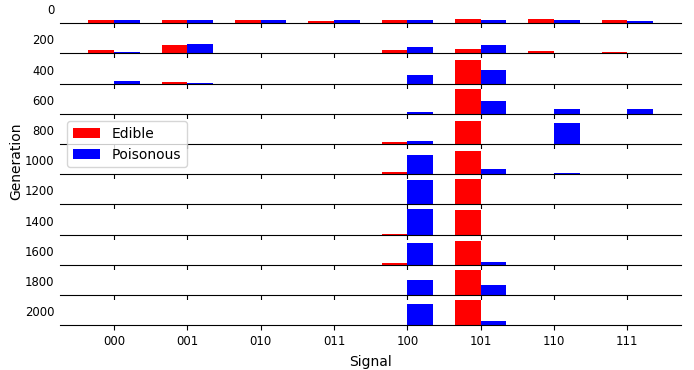
\includegraphics[width=1.\linewidth]{results/language.png}
%          \caption{Frequency distribution of the possible signals produced by all individuals in 10 generations in one replica of a simulation with an \bf{evolved language}.}
%          \label{fig:language-evolved3}
%   \end{minipage}
%   \begin{minipage}{0.49\textwidth}
%          \centering
%          \captionsetup{width=.9\linewidth}
%          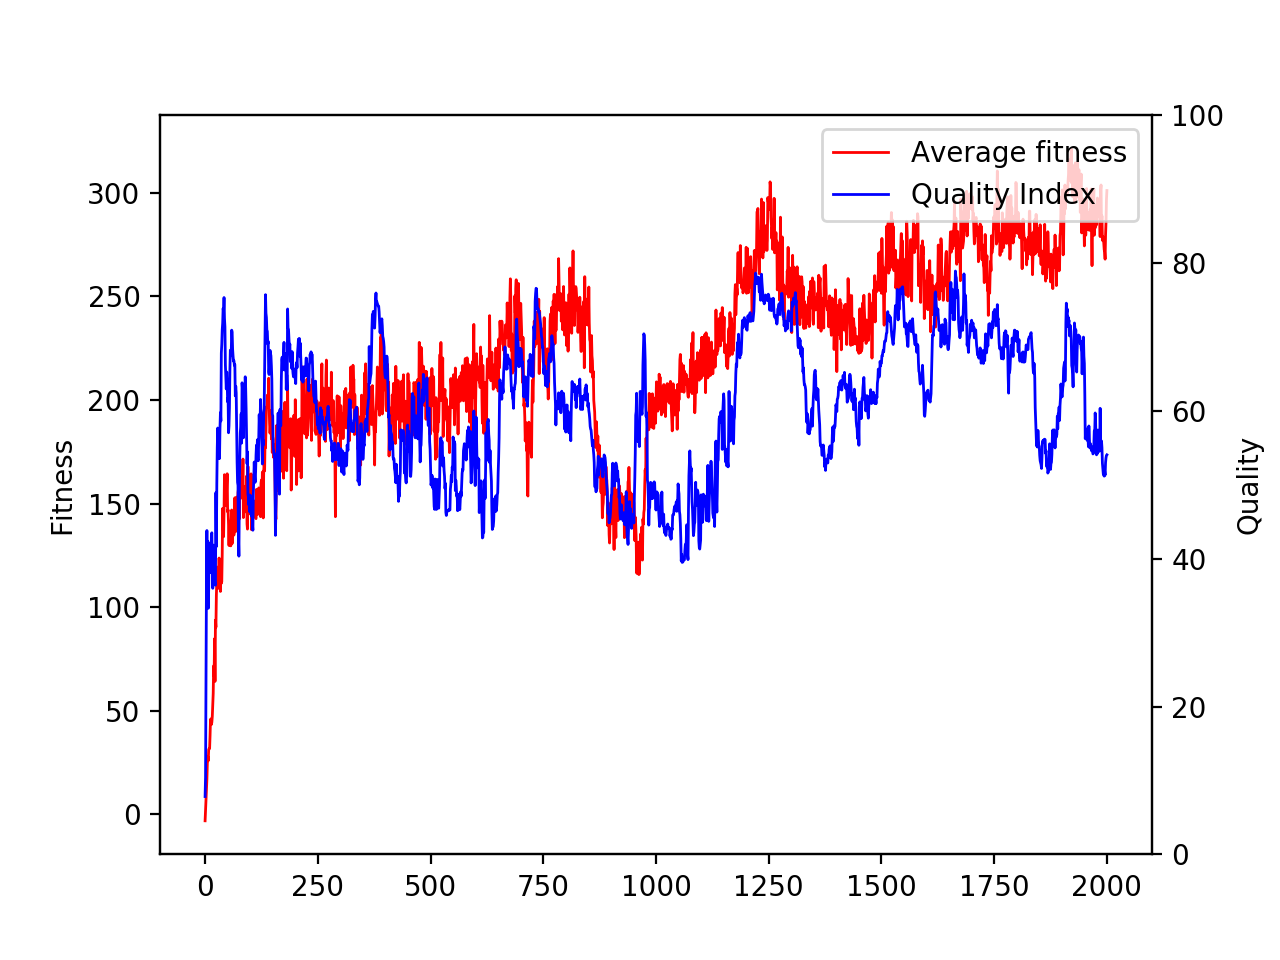
\includegraphics[width=1.\linewidth]{results/correlation.png}
%          \caption{Average fitness for one replica of a population with an {\bf evolved language}. Also shown is the Quality Index score of the language produced by this population.}
%          \label{fig:correlation}
%   \end{minipage}
%\end{figure*}

\begin{figure}[t]
  \centering
  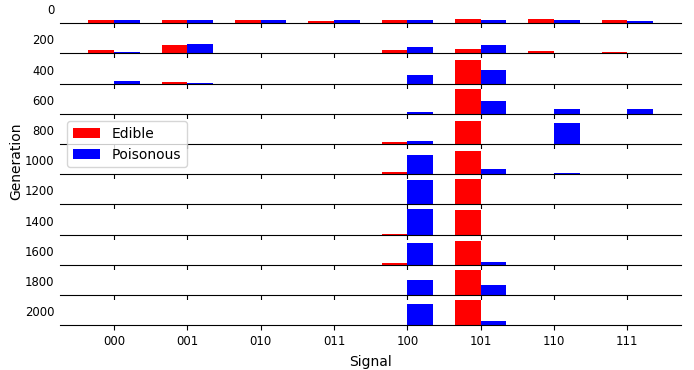
\includegraphics[width=.8\linewidth]{results/language.png}
    \caption{Frequency distribution of the possible signals produced by all individuals in 10 generations in one replica of a simulation with an \bf{evolved language}.}
   \label{fig:language-evolved3}
\end{figure}

\begin{figure}[t]
  \centering
  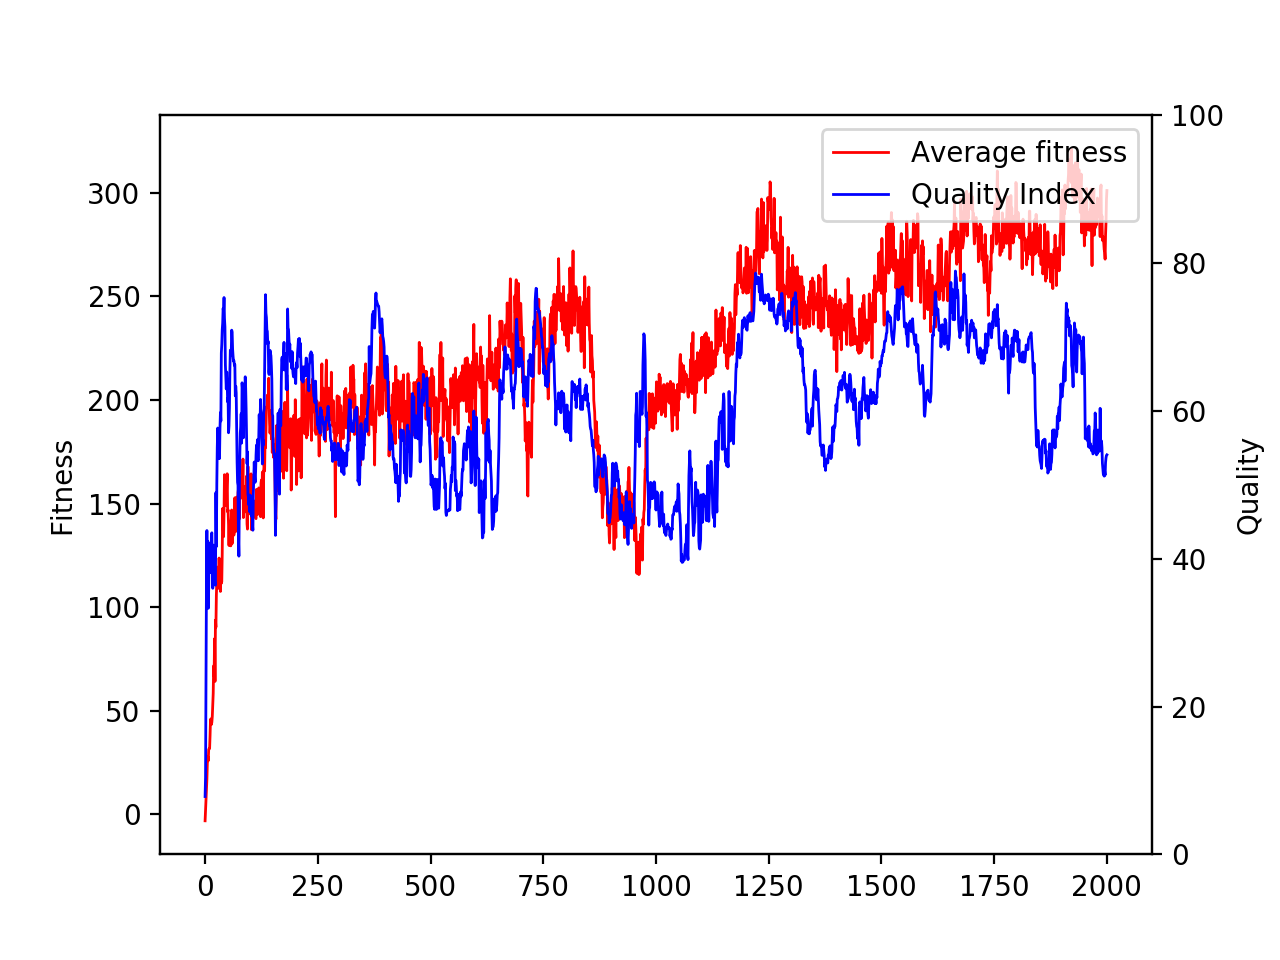
\includegraphics[width=.8\linewidth]{results/correlation.png}
 \caption{Average fitness for one replica of a population with an {\bf evolved language}. Also shown is the Quality Index score of the language produced by this population.}
  \label{fig:correlation}
\end{figure}

\cref{fig:language-evolved3} shows the frequency distribution of the signals produced by one of the replicas from the experiment. The frequency distribution is calculated using the naming task described in \cref{section:efficiency}. The first observation is that at generation 0, the distribution of signals for edible and poisonous mushrooms is flat. This is to be expected, as this results from random weights chosen for all entities in the population. The language at this point provides no information to the listeners in the simulation. Over time, the population converges to using a single signal to label all mushrooms in the same category (criteria 2) and all individuals of the population use the same signals (criteria 3). By generation 400, the majority of the population uses only signals \verb~100~ and \verb~101~ but still struggles to distinguish between the two mushroom types. By generation 1000, criteria 1 is satisfied with signal \verb~100~ used for poisonous mushrooms and signal \verb~101~ for edible. 

In \cref{fig:correlation} we can see how the QI score of the language changes across 2000 generations. Initially the QI score is close to 0, corresponding with the flat distribution seen for generation 0 in \cref{fig:language-evolved3}. This is because this is the least efficient language, providing no information to listeners. The language quality quickly rises as the language converges to a more efficient state, peaking at 80\%. A score of 100\% would correspond to a maximally efficient language, like the {\bf external language}. Note that the Quality Index seems to be correlated to the average fitness of the population, also seen in \cref{fig:correlation}. For this replica, the correlation between fitness and quality was 0.568, calculated using Pearson \emph{r}. This suggests that not only is language a useful addition, but the quality of the language directly affects the resulting evolutionary success of the population.

% COULD SHOW QI CORRELATIONS FOR THE OTHER 9 RUNS 
% COULD SHOW QI SCORES FOR 'NONE' POPULATION AS THEY DID IN THE PAPER
% AND DISCUSS THE PARALLEL CO-EVOLUTION OF LANGUAGE PRODUCTION AND MUSHROOM CATEGORISATION, BUT I DIDN'T GET GOOD RESULTS FOR THIS

\section{Behavioural Analysis}\label{section:behaviouranalysis}

% Talk about convergence of two behaviours in identity population
% Show how the neural network weights converge over time
% Talk abut how identity population can have neural networks compressed
% Show how two clear behaviours have emerged
% Decide to explore different genetic algorithm parameters as a result, link to later section

In \cref{section:popfit} I presented the average fitness of each population over ten replications of the simulation. By examining these ten individual replications we can gain some interesting insight into the evolutionary convergence of different behaviours.

\begin{figure*}[t]
   \centering
   \begin{minipage}{0.49\textwidth}
          \centering
          \captionsetup{width=.9\linewidth}
          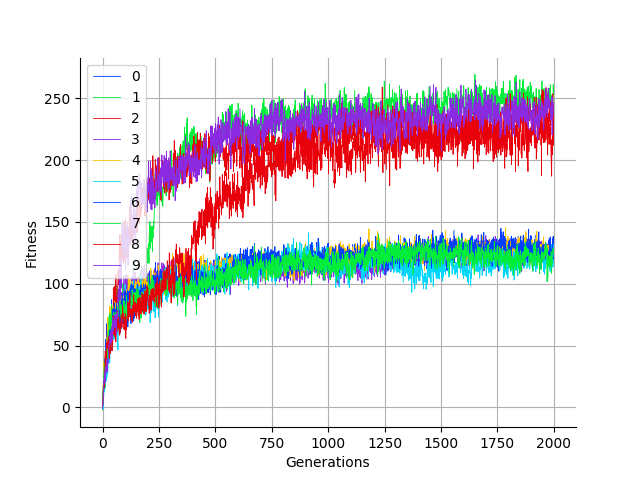
\includegraphics[width=1.\linewidth]{results/ten-none-identity.png}
          \caption{Average fitness of 10 replications of the {\bf no language} population, with an {\bf identity} hidden layer activation.}
          \label{fig:ten-none-identity}
   \end{minipage}
   \begin{minipage}{0.49\textwidth}
          \centering
          \captionsetup{width=.9\linewidth}
          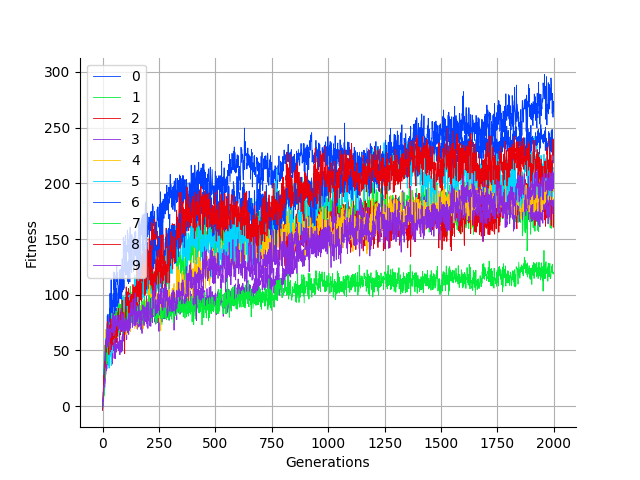
\includegraphics[width=1.\linewidth]{results/ten-none-relu.png}
          \caption{Average fitness of 10 replications of the {\bf no language} population, with a {\bf ReLU} hidden layer activation.}
          \label{fig:ten-none-relu}
   \end{minipage}
\end{figure*}

\cref{fig:ten-none-identity} shows these ten replications for the {\bf no language} population for the experiment using an {\bf identity} activation function on the hidden layer. It seems that the ten populations are converging to two distinct states; four converge to an average fitness of 250 and the other six converge to an average fitness of 125. One of the replications (seen in red) even seems to jump from one state to the other. \cref{fig:ten-none-relu} reveals the ten replicas for the experiment using a {\bf ReLU} activation function which seems to produce more of a continuum of states.

Examining the weights of the neural networks in each population helps provide some understanding. \cref{fig:weights-2000} presents a heatmap of the weights and biases of 100 entities taken from generation 2000 of one of these populations, clamped to [-2, 2]. It is clear from the uniformity that by generation 2000 the population has converged to a single state and that by increasing the absolute values of these weights, the state has been protected from the disrupting effects of mutations, thus preventing the population from converging to a different state. \cref{fig:convergence} shows this convergence process for the same population; weights begin initially random but quickly converge to a single state.

\begin{figure*}[t]
   \centering
   \begin{minipage}{0.49\textwidth}
          \centering
          \captionsetup{width=.9\linewidth}
          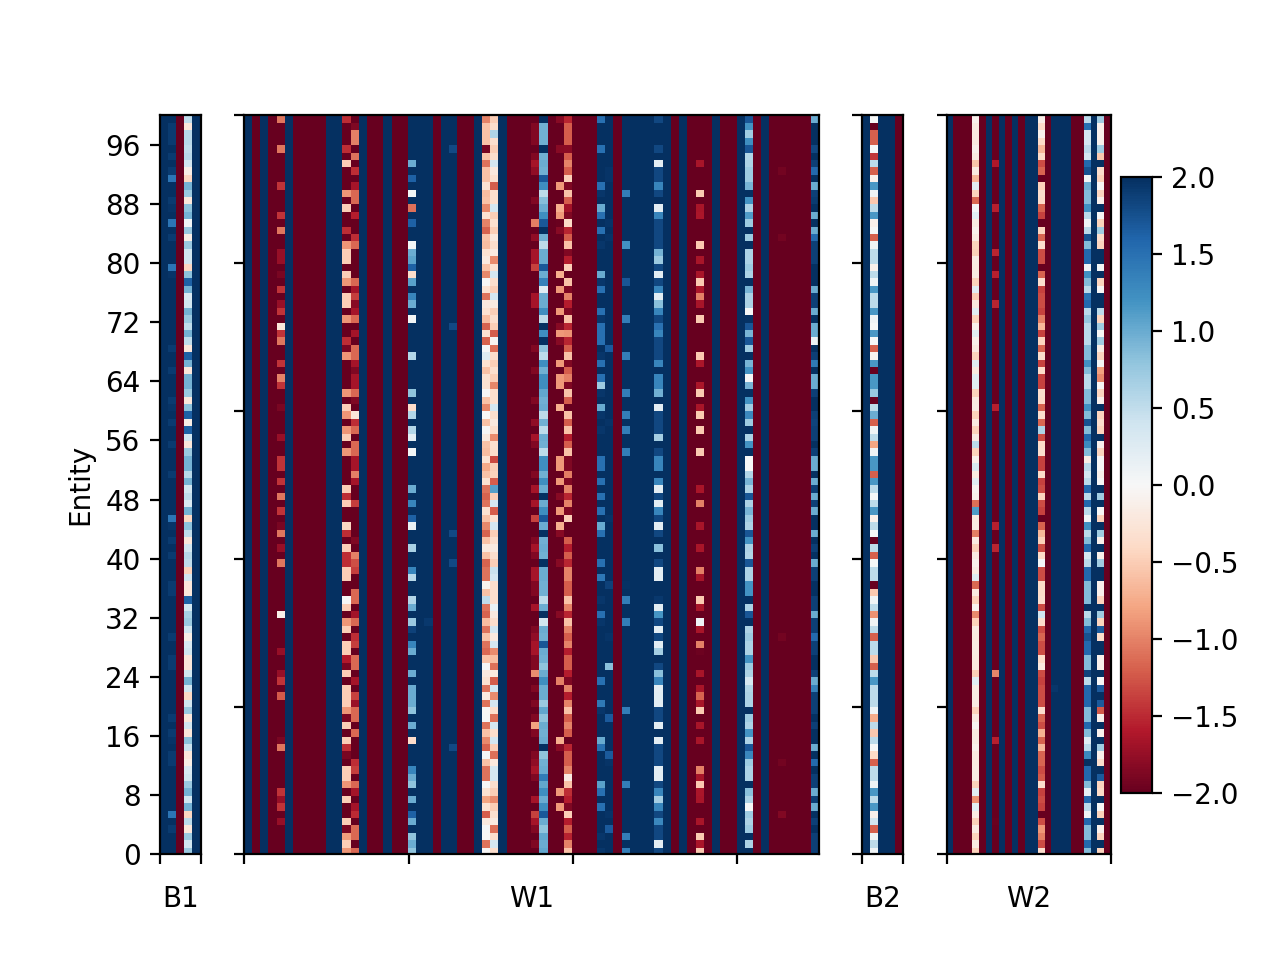
\includegraphics[width=1.\linewidth]{results/weights-2000-none2.png}
          \caption{Heatmap of the weights and biases of 100 entities taken from generation 2000.}
          \label{fig:weights-2000}
   \end{minipage}
   \begin{minipage}{0.49\textwidth}
          \centering
          \captionsetup{width=.9\linewidth}
          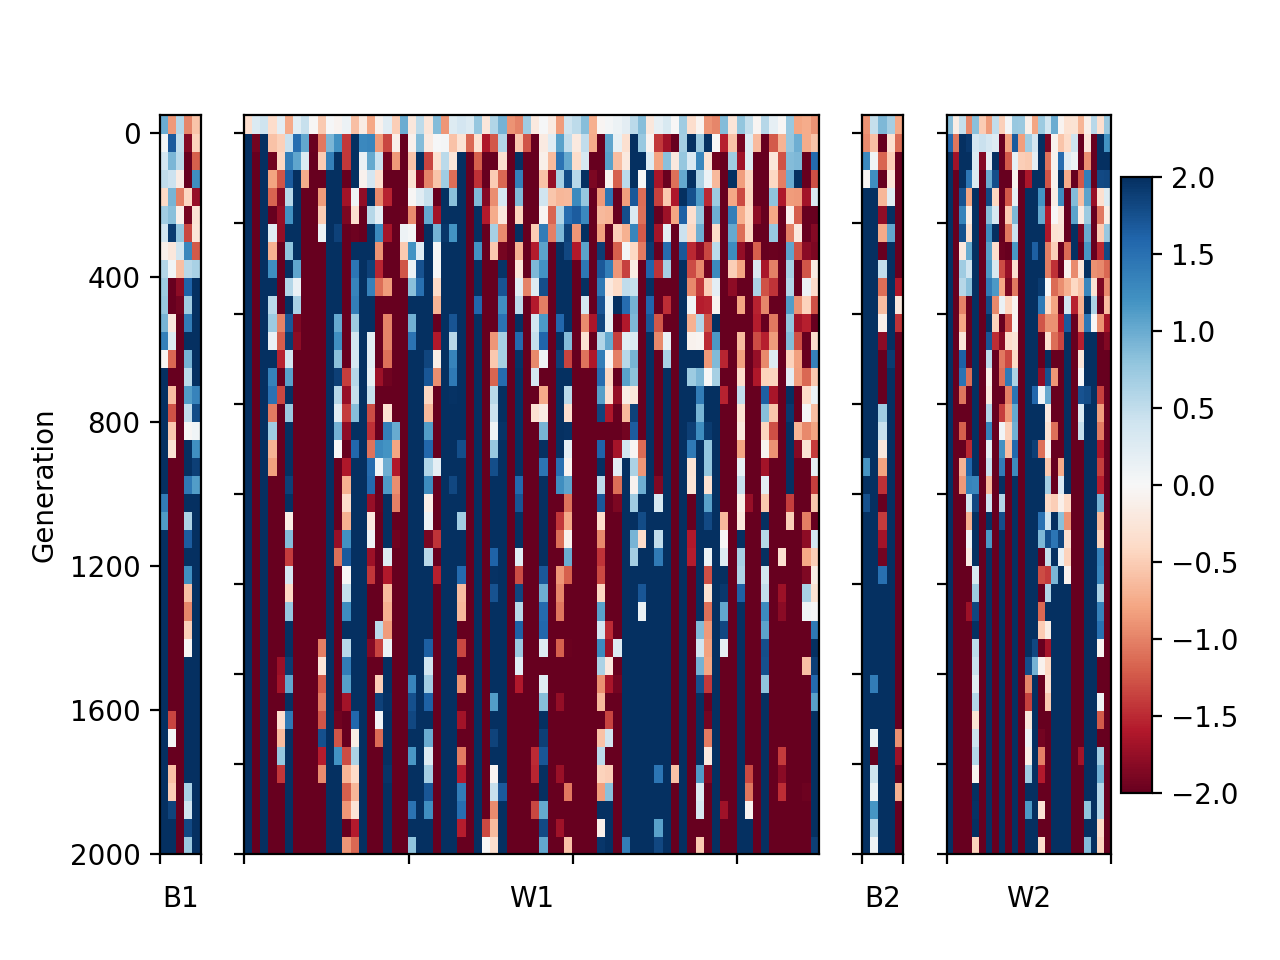
\includegraphics[width=1.\linewidth]{results/convergence.png}
          \caption{Heatmap of a randomly chosen entity taken from increasing generations.}
          \label{fig:convergence}
   \end{minipage}
\end{figure*}

It seems therefore that one set of populations has converged to a better state than the others. Attempting to compare the heatmaps of these different populations does not yield any clear result. Recalling from \cref{section:neural} that the hidden layer is redundant when the identity is used as an activation function, we can produce an equivalent representation of these neural networks by multiplying through the weights and biases of the hidden layer:

$$ W' = W_1 W_0 $$
$$ B' = W_1 B_0 + B_1 $$

where $W_1$, $B_1$, $W_0$ and $B_0$ are the weights and biases for the output layer and hidden layer respectively and $W'$ and $B'$ are the weights and biases for the new, equivalent neural representation. \cref{fig:compare} compares these heatmaps, displaying just the weights and biases that map to the two movement outputs (ignoring the weights and biases that map to the signal outputs). The top set of networks achieved a fitness of close to 250 whereas the bottom six only achieved a fitness of close to 125 but simply examining the neural networks reveals no clear discernible difference between them.

\begin{figure}[t]
  \centering
  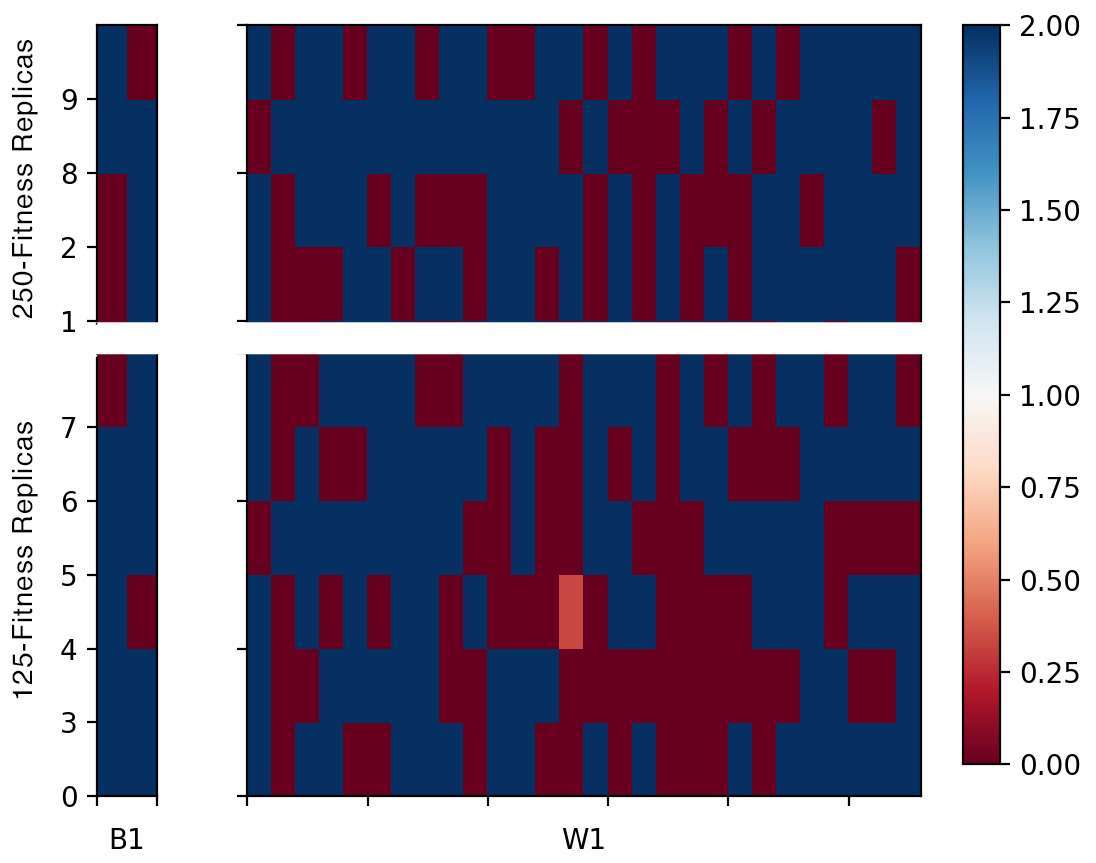
\includegraphics[width=1.\linewidth]{results/compare2}
  \caption{Heatmaps of the flattened neural networks of a randomly chosen entity from generation 2000 of ten replicas.}
  \label{fig:compare}
\end{figure}

Instead, it is productive to examine the actual behaviour exhibited by these ten populations. I examined how each population behaved when faced with a poisonous mushroom. Taking a random entity from generation 2000 of each population, I placed a poisonous mushroom two cells in front of them. As expected, since all ten of these populations have no language, all ten entities moved towards the mushroom until adjacent (they otherwise have no means of categorising the mushroom). Once the mushroom is seen, however, two very different sets of behaviours are exhibited. These are seen in \cref{fig:poisonous-behaviour}.


\begin{figure*}[t]
    \centering
    \begin{minipage}{0.49\textwidth}
        \centering
        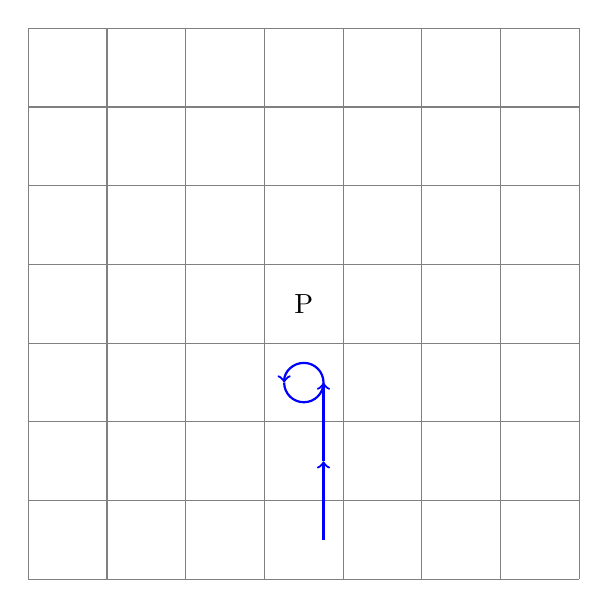
\begin{tikzpicture}
        \draw[step=1cm,color=gray] (0,0) grid (7, 7);
        %\node at (3.5,0.5){$\blacktriangle$};
        \node at (3.5,3.5){P};
        \draw[blue, thick, ->] (3.75,0.5) -- (3.75,1.5);
        \draw[blue, thick, ->] (3.75,1.5) -- (3.75,2.5);
        \draw[blue, thick, ->] (3.25,2.5) arc (-180:180:0.25);
        \end{tikzpicture}
    \end{minipage}\hfill
    \begin{minipage}{0.49\textwidth}
        \centering
        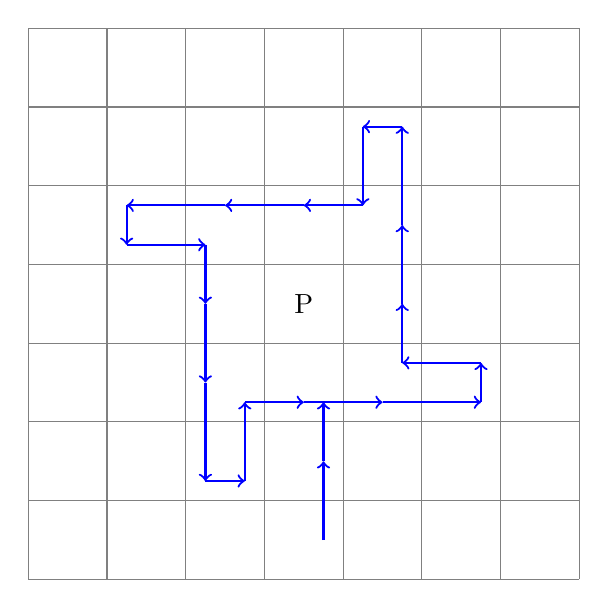
\begin{tikzpicture}
        \draw[step=1cm,color=gray] (0,0) grid (7, 7);
        %\node at (3.25,0.25){$\blacktriangle$};
        \node at (3.5,3.5){P};
        \draw[blue, thick, ->] (3.75,0.5) -- (3.75,1.5);
        \draw[blue, thick, ->] (3.75,1.5) -- (3.75,2.25);
        \draw[blue, thick, ->] (3.5,2.25) -- (4.5,2.25);
        \draw[blue, thick, ->] (4.5,2.25) -- (5.75,2.25);
        \draw[blue, thick, ->] (5.75,2.25) -- (5.75,2.75);
        \draw[blue, thick, ->] (5.75,2.75) -- (4.75,2.75);
        \draw[blue, thick, ->] (4.75,2.75) -- (4.75, 3.5);
        \draw[blue, thick, ->] (4.75,3.5) -- (4.75,4.5);
        \draw[blue, thick, ->] (4.75,4.5) -- (4.75,5.75);
        \draw[blue, thick, ->] (4.75,5.75) -- (4.25,5.75);
        \draw[blue, thick, ->] (4.25,5.75) -- (4.25,4.75);
        \draw[blue, thick, ->] (4.25,4.75) -- (3.5,4.75);
        \draw[blue, thick, ->] (3.5,4.75) -- (2.5,4.75);
        \draw[blue, thick, ->] (2.5,4.75) -- (1.25,4.75);
        \draw[blue, thick, ->] (1.25,4.75) -- (1.25,4.25);
        \draw[blue, thick, ->] (1.25,4.25) -- (2.25,4.25);
        \draw[blue, thick, ->] (2.25,4.25) -- (2.25,3.5);
        \draw[blue, thick, ->] (2.25,3.5) -- (2.25,2.5);
        \draw[blue, thick, ->] (2.25,2.5) -- (2.25,1.25);
        \draw[blue, thick, ->] (2.25,1.25) -- (2.75,1.25);
        \draw[blue, thick, ->] (2.75,1.25) -- (2.75,2.25);
        \draw[blue, thick, ->] (2.75,2.25) -- (3.5,2.25);
    \end{tikzpicture}
    \end{minipage}
    \caption{The behaviour of two entities approaching a poisonous mushroom (P). The entities are randomly chosen from generation 2000 of two {\bf no language} populations with an average fitness of 140 (left) and 250 (right).}
    \label{fig:poisonous-behaviour}
\end{figure*}

The six populations that achieved a maximum fitness of 150 all exhibited ``stuck'' behaviours. Four of these populations spun in place (either clockwise or anti-clockwise) and the other two produced the \verb~None~ action indefinitely. Whilst valid means of avoiding the poisonous mushrooms, I call these behaviours ``stuck'' as it prevents the entity from discovering more mushrooms.

The other four populations, those that achieve a fitness of 250, exhibit ``exploratory'' behaviours. All four entities moved in the symmetric path seen in \cref{fig:poisonous-behaviour}, again either clockwise or anti-clockwise. This behaviour also allows the entity to avoid the mushroom but also allows it to potentially discover a different mushroom and continue searching; explaining how a higher fitness is achieved. 

Examining these populations at generation 200 reveals the same behaviours except for one population; replica 8 now exhibits the ``stuck'' behaviour. At generation 250 however, replica 8 has switched to the ``exploratory'' behaviour. This seems to correspond with the `jump' to the higher state seen in \cref{fig:ten-none-identity}. From this we can conclude that early in the evolution, some populations converge to more productive behaviours than others and the gradual strengthening of weights prevents the lesser populations from escaping these states.

The same behavioural analysis can also be applied to the ten replicas seen in \cref{fig:ten-none-relu}. Although these form more of a continuum of states, similar behaviours are noticed. The green line corresponding with the 120-fitness population exhibits ``stuck'' behaviour whilst the blue line corresponding with the 280-fitness population exhibits ``exploratory'' behaviour with an even broader search path than seen in \cref{fig:poisonous-behaviour}. It seems that for the populations without language, it is the search strategy that determines genetic success.

\section{Exploring Simulation Parameters}\label{section:simulation-parameters}

Throughout Chapter 2 and 3, I discussed how the many design elements of the simulation were fairly arbitrary. One example is equation to calculate fitness:

$$\mathrm{F} = 10 E - 11 P$$

Although the scaling parameters of the equation seem arbitrary, they do not make a difference. This is because by generation 1000 all populations successfully avoid poisonous mushrooms and so it is the searching ability that determines the differences in fitness. Removing the $P$ term entirely would make a difference however as it would remove the penalty of eating a poisonous mushroom, leading to alternative behaviours.

Another arbitrary choice is the implementation decision I made about when an entity attempts to walk through the edge of the world. Instead of the entities getting stuck, I could have them `bounce-back' or loop to the other side. When these alternative behaviours were implemented, no difference was found in the results besides an overall scaling of each curve. This is because the entities cannot detect the edge of the world; running into an edge is a random event so allowing them to pass through or bounce back only increases their exploration time.

The majority of arbitrary choices can be found in the simulation parameters, those found in \cref{table:constants}. \cref{section:popfit} demonstrated that the simulation was robust to the activation function was used in the hidden layer of the neural networks. In all cases, the populations with language performed better than those without. In this the remainder of this section, I will explore the effect of changing neural network depth, adjusting the length of each epoch and altering the genetic algorithm parameters.

\subsection{Neural Network Depth}

\begin{figure*}[t]
   \centering
   \begin{minipage}{0.49\textwidth}
          \centering
          \captionsetup{width=.9\linewidth}
          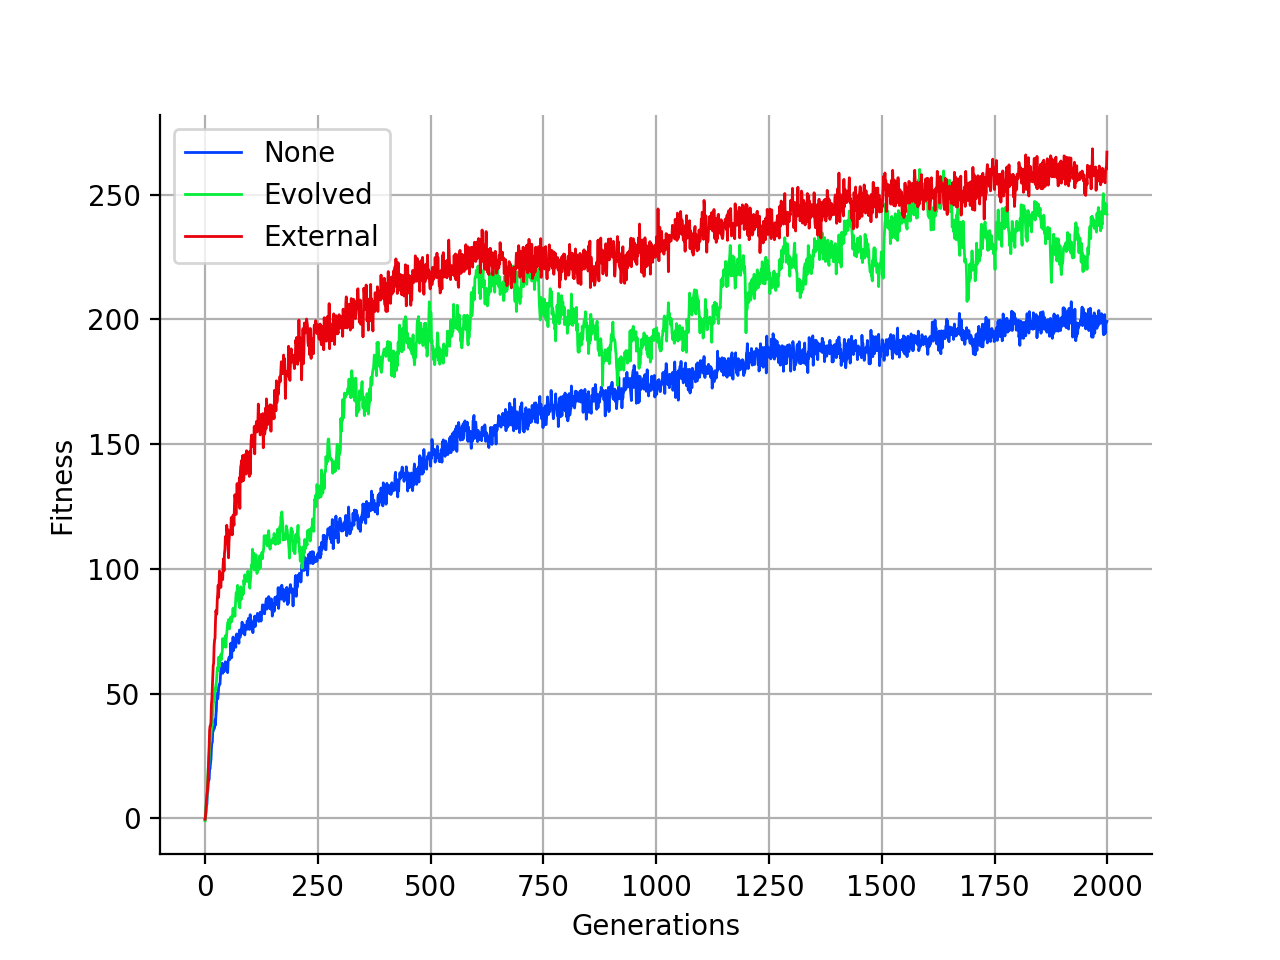
\includegraphics[width=1.\linewidth]{results/average-55.png}
          \caption{Average fitness of each population, averaged over 10 replications, with two hidden layers of five units each.}
          \label{fig:average-55}
   \end{minipage}
   \begin{minipage}{0.49\textwidth}
          \centering
          \captionsetup{width=.9\linewidth}
          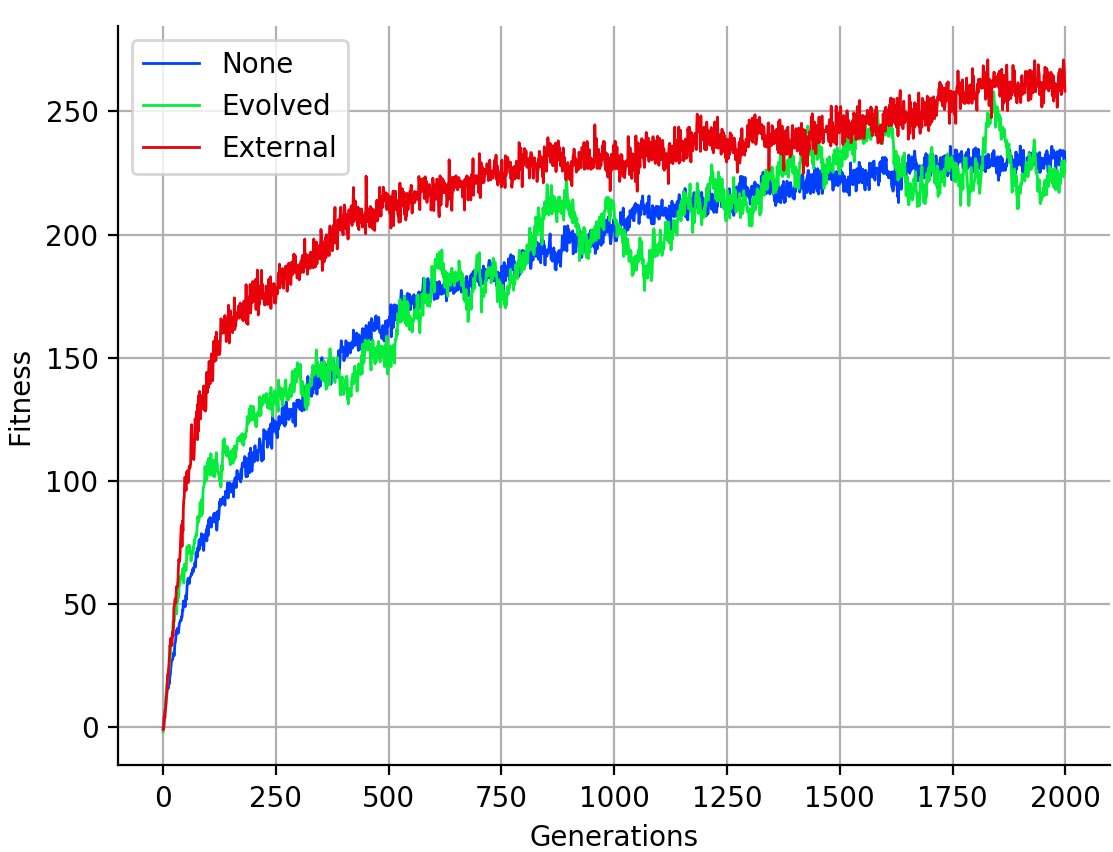
\includegraphics[width=1.\linewidth]{results/average-10510.png}
          \caption{Average fitness of each population, averaged over 10 replications, with three hidden layers of ten units, five units and ten units.}
          \label{fig:average-10510}
   \end{minipage}
\end{figure*}

I first wanted to explore whether increasing the depth of the neural networks would affect the performance of the populations. Taking the exact same parameters as my initial experiment and increasing the depth of the neural network to contain \emph{two} hidden layers of five units each gives us \cref{fig:average-55}. Comparing these results to \cref{fig:average-relu} does not reveal much difference; the {\bf evolved language} and {\bf no language} populations still reach fitnesses of 250 and 200 respectively, with the {\bf evolved language} populations also reaching 250. Examining an even deeper network (\cref{fig:average-10510}) presents a situation where the population without language performs much better, even surpassing the population with an evolved language. Performing behavioural analysis of these populations, as in \cref{section:behaviouranalysis}, reveals that this is just occurring because nine out of the ten replicas are reaching the ``exploratory'' state with only one in the ``stuck'' state, thus increasing the average shown in this figure. The low performance of the {\bf evolved language} populations is likely due to the hugely increased number of weights and biases introduced by this experiment (320 instead of 105), increasing the learning time required for these populations to develop an efficient language and reach good evolutionary performance. Examining the language produced by these populations reveals that convergence is much slower. It seems that adding in more layers has allowed these populations to escape local minima but has not allowed them to discover more sophisticated behaviours.

\subsection{Epoch Length}

\cref{table:constants} lists the seemingly arbitrary simulation parameters specified by \citet{Cangelosi1998}. Observing the effect of these parameters on the outcome of the simulation can produce some insight into whether these parameters are in fact arbitrarily chosen, perhaps to produce good results or whether the simulation is robust to these changes.

\begin{figure*}[t]
   \centering
   \begin{minipage}{0.49\textwidth}
          \centering
          \captionsetup{width=.9\linewidth}
          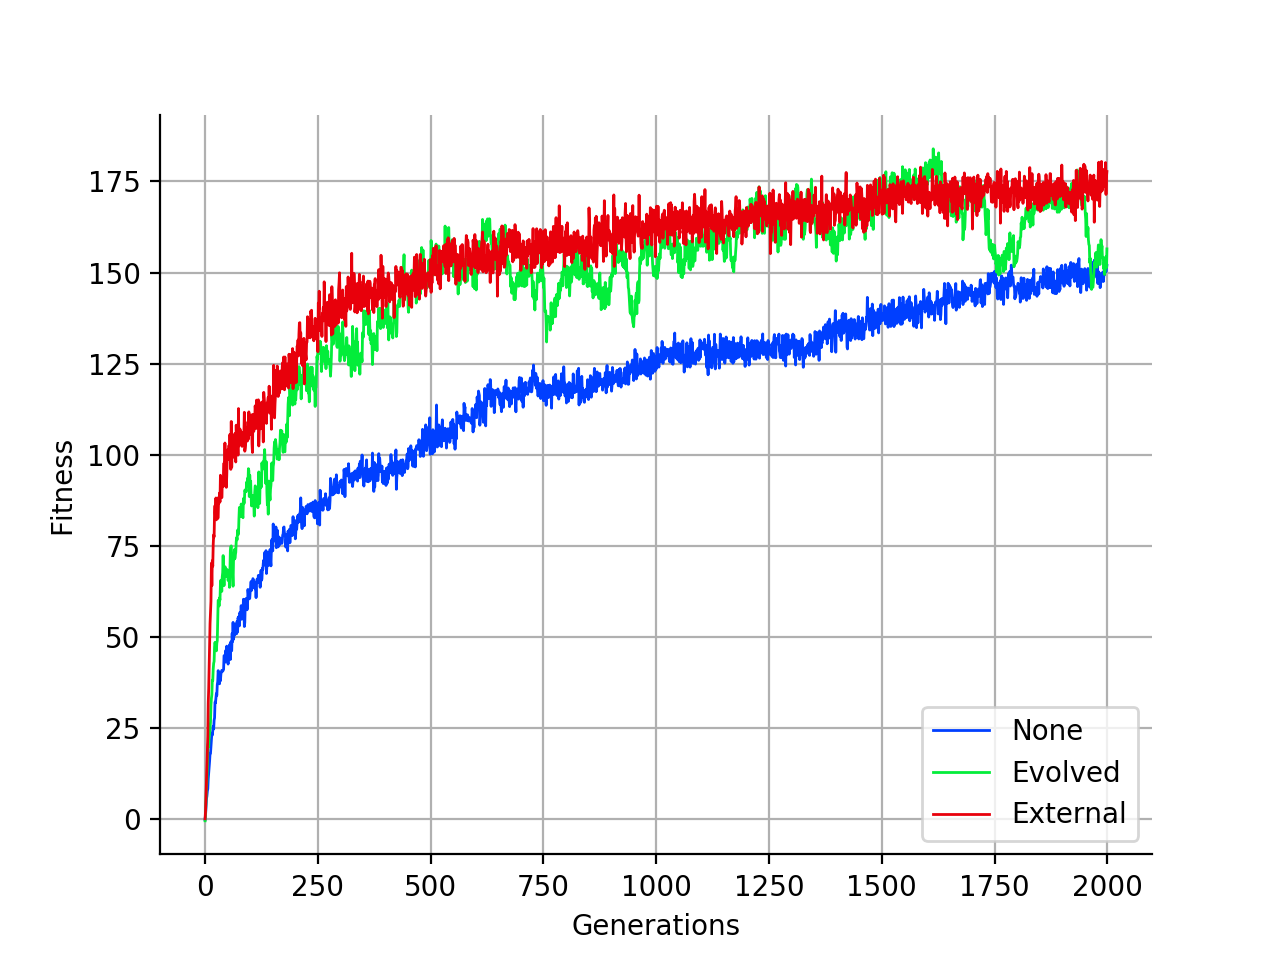
\includegraphics[width=1.\linewidth]{results/average-short-epo.png}
          \caption{Average fitness of each population, averaged over 10 replications, with simulations consisting of 30 epochs of length 15.}
          \label{fig:average-short-epo}
   \end{minipage}
   \begin{minipage}{0.49\textwidth}
          \centering
          \captionsetup{width=.9\linewidth}
          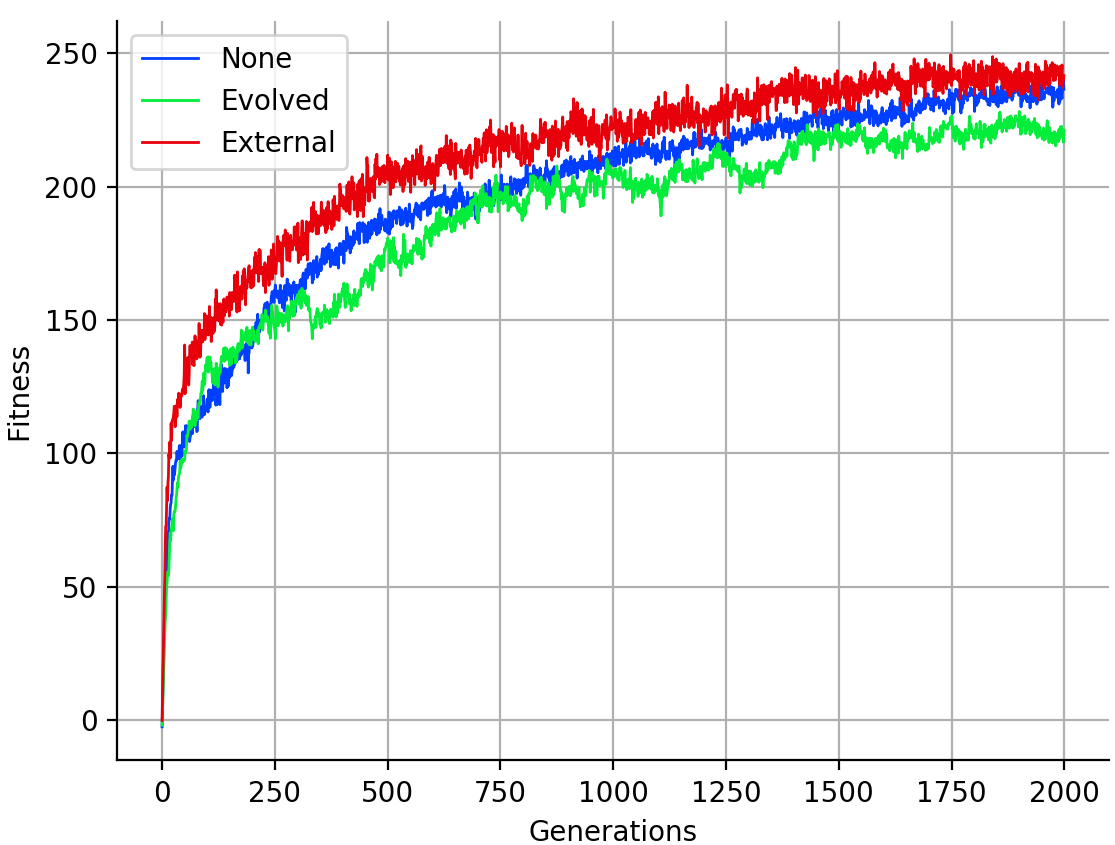
\includegraphics[width=1.\linewidth]{results/average-long-epo.png}
          \caption{Average fitness of each population, averaged over 10 replications, with simulations consisting of 10 epochs of length 75.}
          \label{fig:average-long-epo}
   \end{minipage}
\end{figure*}

I first experimented with changing the duration of each epoch while keeping the total number of cycles constant. In \cref{fig:average-short-epo} we do not observe much change in the comparison between the three populations although the fitness scores achieved are lower for all three populations. With only 15 cycles per epoch, it is likely that this prevents the entities from reaching more than one edible mushroom in each cycle. Increasing the number of cycles per epoch to 75 gives us \cref{fig:average-long-epo}. Here we get very different results; the three populations achieve very similar fitness scores and the population with {\bf no language} performs better than the population with the {\bf evolved language}. This can similarly be explained from the duration of the epochs; with more time to explore, the advantage of having mushrooms labelled before approach is reduced, resulting in similar fitness scores. This does, however, show that the simulation setup is not fully robust to changes in parameters.
 
 \subsection{Genetic Parameters}
 
\begin{figure*}[ht]
   \centering
   \begin{minipage}{0.49\textwidth}
          \centering
          \captionsetup{width=.9\linewidth}
          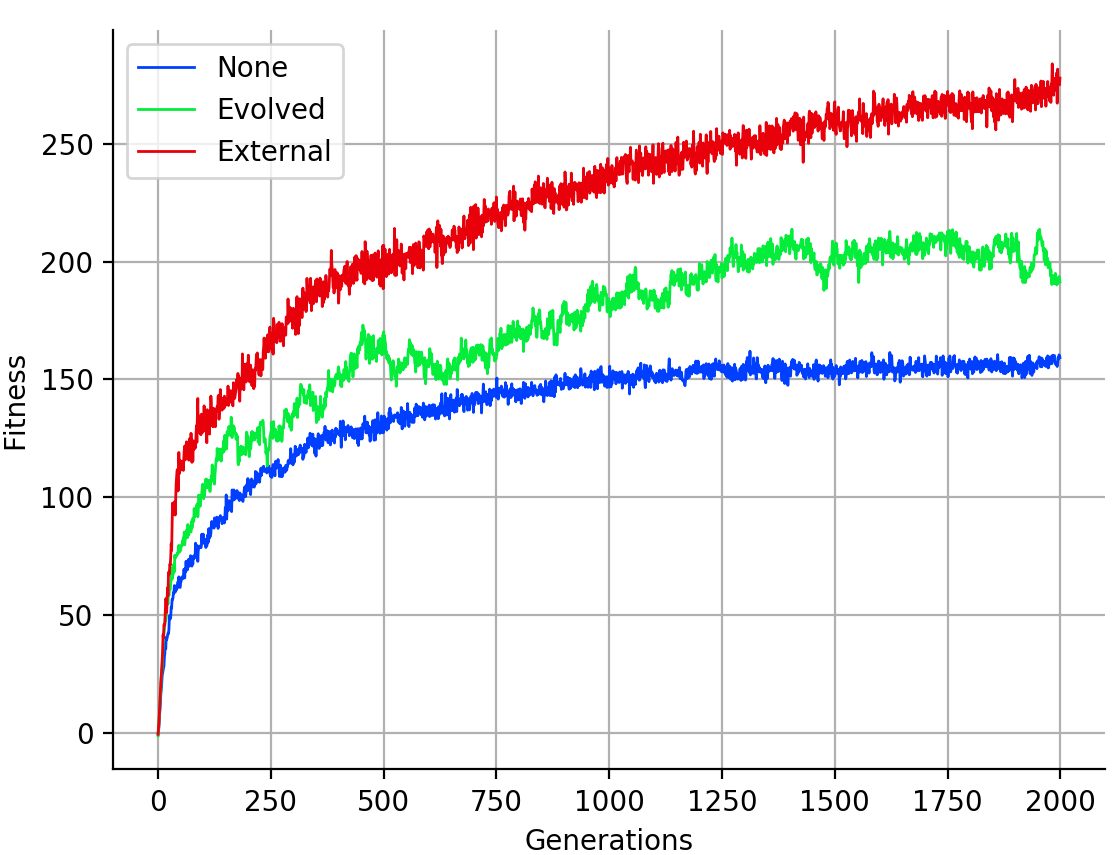
\includegraphics[width=1.\linewidth]{results/average-mut20.png}
          \caption{Average fitness of each population, averaged over 10 replications, with the mutation percentage set to 20\%.}
          \label{fig:average-mut20}
   \end{minipage}
   \begin{minipage}{0.49\textwidth}
          \centering
          \captionsetup{width=.9\linewidth}
          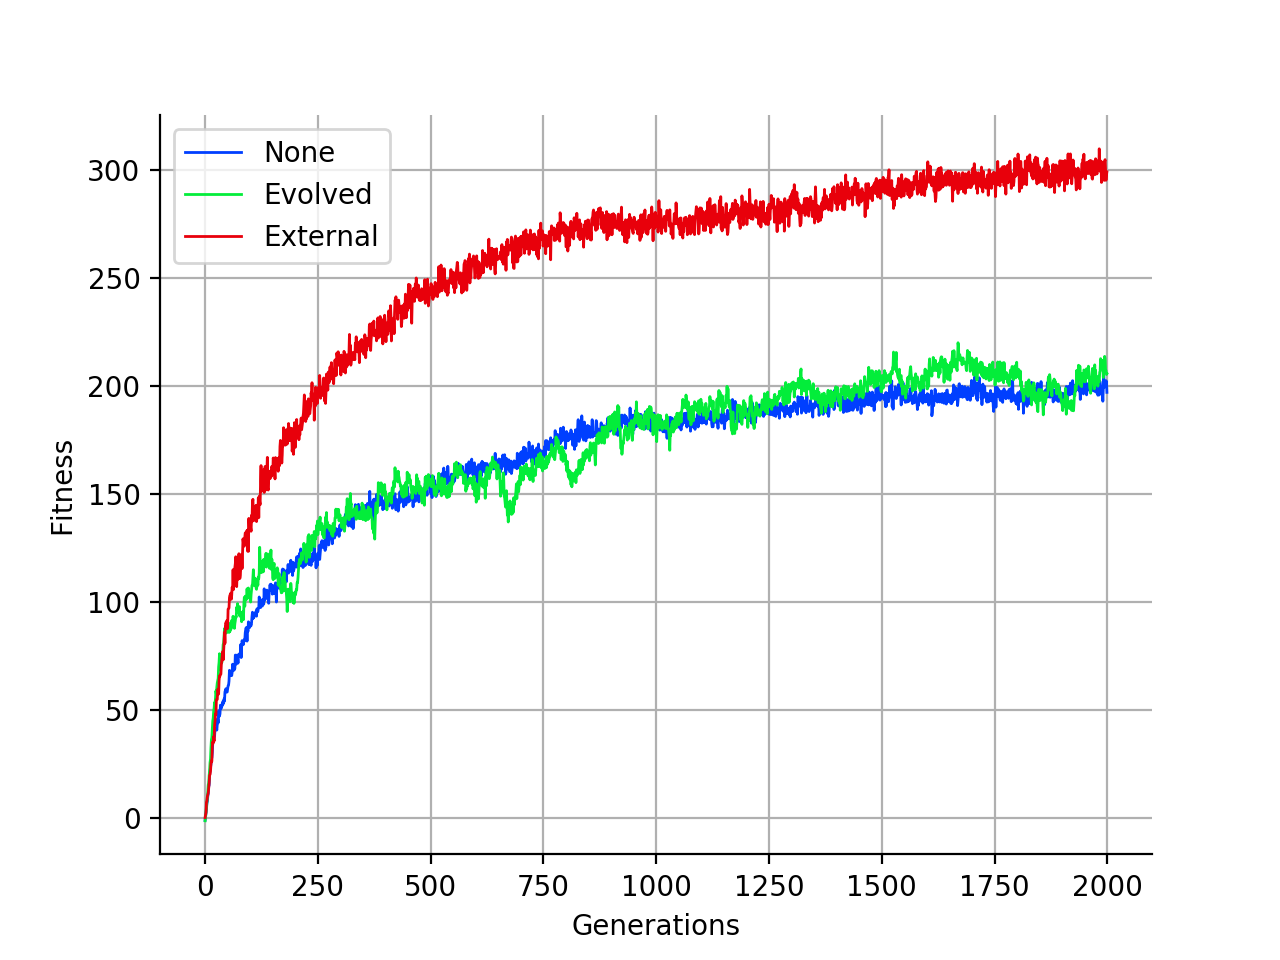
\includegraphics[width=1.\linewidth]{results/average-mut50.png}
          \caption{Average fitness of each population, averaged over 10 replications, with the mutation percentage set to 50\%.}
          \label{fig:average-mut50}
   \end{minipage}
\end{figure*}

\begin{figure*}[ht]
   \centering
   \begin{minipage}{0.49\textwidth}
          \centering
          \captionsetup{width=.9\linewidth}
          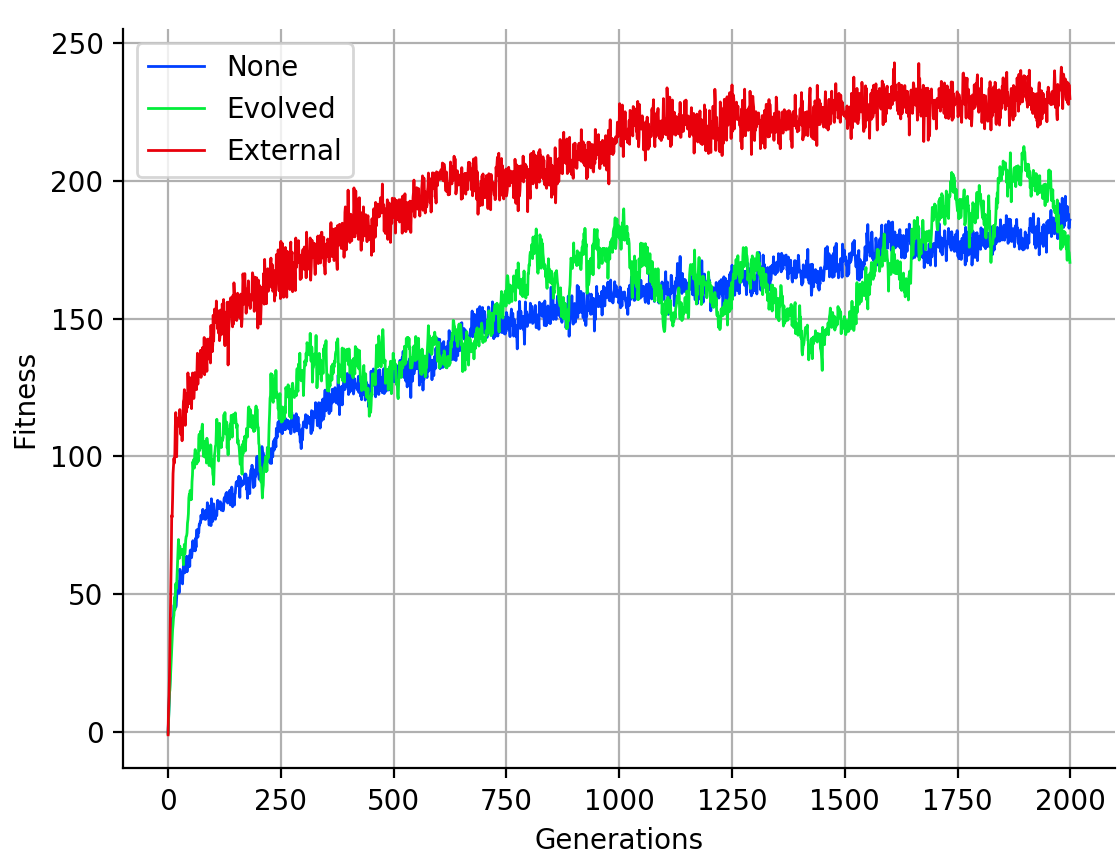
\includegraphics[width=1.\linewidth]{results/average-keep10.png}
          \caption{Average fitness of each population, averaged over 10 replications, with the percentage of entities selected to reproduce set to 10\%.}
          \label{fig:average-keep10}
   \end{minipage}
   \begin{minipage}{0.49\textwidth}
          \centering
          \captionsetup{width=.9\linewidth}
          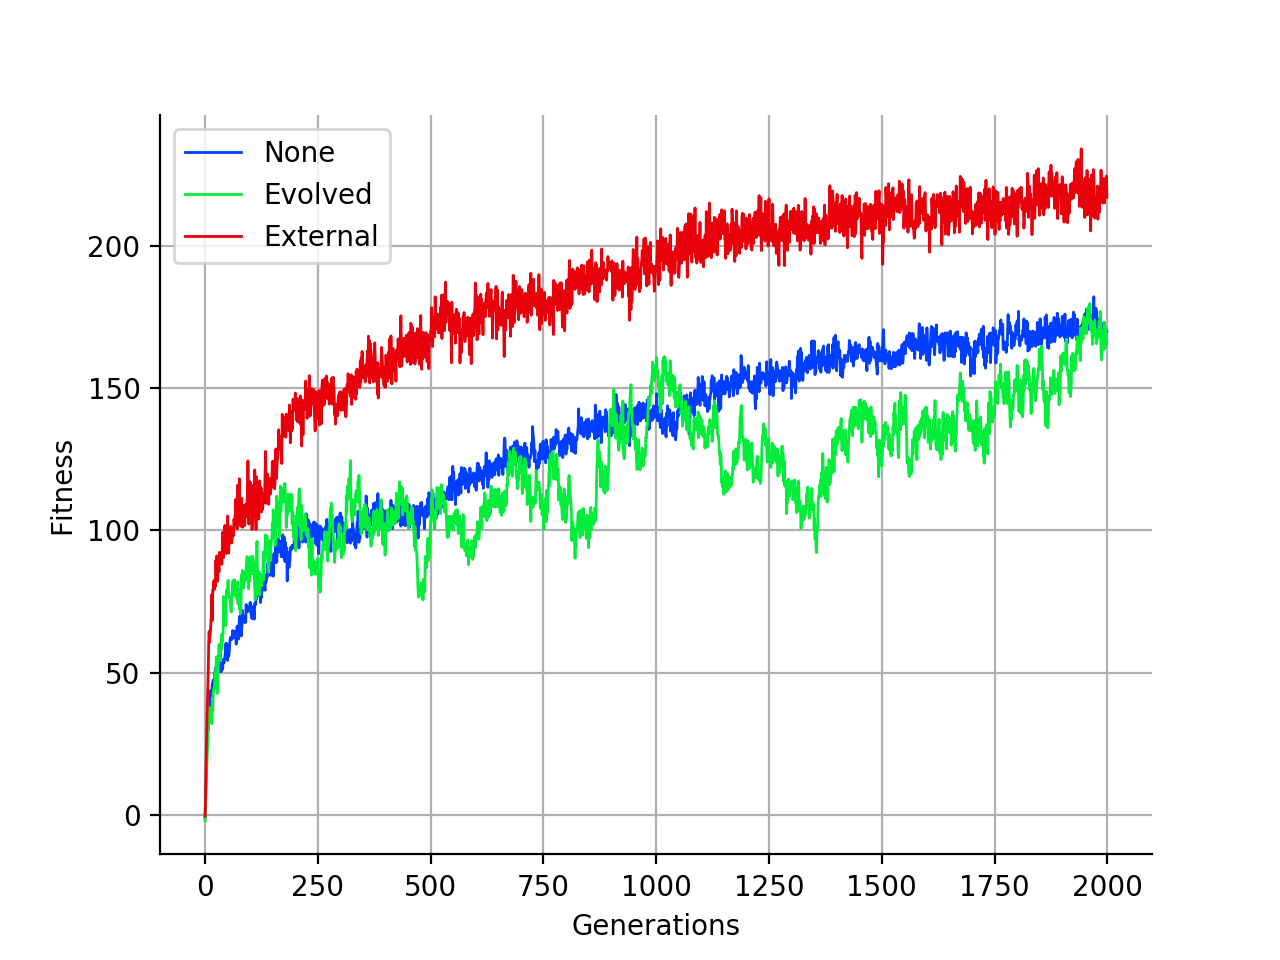
\includegraphics[width=1.\linewidth]{results/average-keep05.png}
          \caption{Average fitness of each population, averaged over 10 replications, with the percentage of entities selected to reproduce set to 5\%.}
          \label{fig:average-keep05}
   \end{minipage}
\end{figure*}
 
Following the behavioural analysis in \cref{section:behaviouranalysis}, it is worth exploring how changing the parameters of the genetic algorithm may affect the observed convergence to two different behaviours in the {\bf no language} populations.

Figures \ref{fig:average-mut20} and \ref{fig:average-mut50} present the effect of increasing the mutation percentage to from 10\% to 20\% and 50\% respectively and Figures \ref{fig:average-keep10} and \ref{fig:average-keep05} present the effect of reducing the percentage of entities chosen for reproduction from 20\% to 10\% and 5\% respectively. It seems as if each population type is affected by these changes differently, for example the reduction in the percentage of entities kept between generations negatively affects the two populations with language but does not seem to have an effect on the population without language; resulting in the {\bf evolved language} population performing worse than the population with {\bf no language}. In my opinion, this is because lowering this parameter prevents the emergence of new behaviours and the two populations with language require the emergence of more complex behaviours to take advantage of the additional information. The main observation is that a slight change in these parameters results in very different outcomes to our initial experiment seen in \cref{fig:average-relu}, suggesting that these parameters may have been tuned to maximise the gap between populations with language and those without.

It is worth pointing out that in all of of these experiments, we always see that the {\bf external language} populations perform better than the {\bf no language} populations. What seems to vary between these parameter changes is the performance of the {\bf evolved language} population with respect to these two. With certain changes to the parameters, such as increasing the neural network depth or increasing the mutation percentage, the {\bf evolved language} populations do not seem to converge to a productive language and do not gain an advantage in the mushroom world. Thus, although the simulation does demonstrate that language is always beneficial, it is not fully robust to changes in simulation parameters.

 \section{Summary}
 
Cangelosi and Parisi demonstrated that language is a useful adaptation in the ``mushroom world'' simulation. By implementing this simulation and through the analysis in \cref{section:popfit}, we have seen that this conclusion holds and we have demonstrated that an efficient language emerges through the simulated evolution.

What Cangelosi and Parisi did not analyse was how robust these conclusions were with respect to the many arbitrary design decisions made. Through the analysis made in \cref{section:simulation-parameters}, we have seen that although the main conclusion still holds, the simulation is not robust to these changes and in particular the {\bf evolved language} and {\bf external language} are not equivalent as was suggested by Cangelosi and Parisi in \cref{fig:cangelosi-results}.

Finally, Cangelosi and Parisi also seemed to have missed the convergence of different exploratory behaviours. In \cref{section:behaviouranalysis} we saw that two clear behaviours emerge in the population without language and that these can directly explain the fitness achieved, suggesting that exploration ability may be as important as mushroom categorisation to achieve evolutionary success in this model.

%%%%%%%%%%%%%%%%%%%%%%%%%%%%%%%%%%%%%%%%%%%%%%%%%%%%%%%%%%%%%%%%%%%%%%%
%%%%%%%%%%%%%%%%%%%%%%%%%%%%%%%%%%%%%%%%%%%%%%%%%%%%%%%%%%%%%%%%%%%%%%%
%%%%%%%%%%%%%%%%%%%%%%%%%%%%%%%%%%%%%%%%%%%%%%%%%%%%%%%%%%%%%%%%%%%%%%%
%%%%%%%%%%%%%%%%%%%%%%%%%%%%%%%%%%%%%%%%%%%%%%%%%%%%%%%%%%%%%%%%%%%%%%%
%%%%%%%%%%%%%%%%%%%%%%%%%%%%%%%%%%%%%%%%%%%%%%%%%%%%%%%%%%%%%%%%%%%%%%%
%%%%%%%%%%%%%%%%%%%%%%%%%%%%%%%%%%%%%%%%%%%%%%%%%%%%%%%%%%%%%%%%%%%%%%%
%%%%%%%%%%%%%%%%%%%%%%%%%%%%%%%%%%%%%%%%%%%%%%%%%%%%%%%%%%%%%%%%%%%%%%%
%%%%%%%%%%%%%%%%%%%%%%%%%%%%%%%%%%%%%%%%%%%%%%%%%%%%%%%%%%%%%%%%%%%%%%%
% Conclusion

\chapter{Conclusion}

This project was a success. All points listed in the success criteria and all items in the requirements analysis (\cref{section:requirements}) were completed.

The purpose of this project was to implement the ``toy mushroom world'' simulation described in \citet{Cangelosi1998} and use it to investigate the evolution of a simple one-utterance language used to distinguish between edible and poisonous mushrooms. Entities controlled by neural networks exhibit either no language, an externally provided language or an evolved language and a genetic algorithm simulates evolution over many generations. These entities, the toy world they exist in and the genetic algorithm were all implemented successfully. Throughout the project, good software engineering practices were adhered to, including:
\begin{itemize}
    \item issue tracking
    \item schedule management
    \item a suite of unit tests
    \item continuous integration to prevent the re-emergence of bugs
\end{itemize}

I investigated the behaviour of the simulation according to the metrics described by \citet{Cangelosi1998}. I was able to reproduce the conclusion that populations perform better with language and furthermore that there is a correlation between language quality and fitness. I then performed additional analysis beyond this, analysing the weights of the neural networks and conducting behavioural tests to explain why different populations exhibit two seemingly distinct sets of behaviours. Finally, I explored the robustness of the system to changes made to the simulation parameters, seeking to see if these were tuned by Cangelosi and Parisi to exhibit particular results. From this I discovered that the resulting populations are in fact sensitive to these changes but that the main conclusions still hold.

\section{Lessons Learnt}

The main issue I faced was the emergence of strange behaviours at the population level of the simulation due to small underlying bugs in the core implementation of the entities and the environment objects. This was despite having implemented an extensive suite of unit tests; the problem was unforeseen. Once discovered, I was able to create regression tests to prevent their re-emergence.

Another useful change was the implementation of a command-line interface for my system. Earlier in development, I created hard-coded methods for each experiment that required code changes between each run on the HPC. This slowed the evaluation cycle and resulted in many failed attempts when parameters were not set correctly or were changed before the jobs were scheduled. Introducing the command-line interface allowed me to schedule a dozen experiments at once without touching the code at all.

Finally, during the course of the project I found that Python's dynamic typing introduced very subtle bugs that could not be discovered at compilation-time. This led me to conclude that Python would not be suitable if the aim of this project was to produce industry software, however for the scale of this project I believe that Python was a good choice. The powerful libraries lended themselves well and the dynamic typing lended itself to quick early implementation.

\section{Further Work}

Through the implementation and resulting analysis of this simulation I have demonstrated that computer simulations are a useful tool in the field of language evolution and that interesting behaviours can emerge from even the most basic neural networks. With further time I would seek to implement more expansive simulations to attempt to explain the emergence of linguistic phenomena including verb-object structures and compositionality. I would also seek to create a visual interface for the system to allow the simulation to be used as a learning tool for students interested in learning more about agent-based modelling. 

%%%%%%%%%%%%%%%%%%%%%%%%%%%%%%%%%%%%%%%%%%%%%%%%%%%%%%%%%%%%%%%%%%%%%%%
%%%%%%%%%%%%%%%%%%%%%%%%%%%%%%%%%%%%%%%%%%%%%%%%%%%%%%%%%%%%%%%%%%%%%%%
%%%%%%%%%%%%%%%%%%%%%%%%%%%%%%%%%%%%%%%%%%%%%%%%%%%%%%%%%%%%%%%%%%%%%%%
%%%%%%%%%%%%%%%%%%%%%%%%%%%%%%%%%%%%%%%%%%%%%%%%%%%%%%%%%%%%%%%%%%%%%%%
%%%%%%%%%%%%%%%%%%%%%%%%%%%%%%%%%%%%%%%%%%%%%%%%%%%%%%%%%%%%%%%%%%%%%%%
%%%%%%%%%%%%%%%%%%%%%%%%%%%%%%%%%%%%%%%%%%%%%%%%%%%%%%%%%%%%%%%%%%%%%%%
%%%%%%%%%%%%%%%%%%%%%%%%%%%%%%%%%%%%%%%%%%%%%%%%%%%%%%%%%%%%%%%%%%%%%%%
%%%%%%%%%%%%%%%%%%%%%%%%%%%%%%%%%%%%%%%%%%%%%%%%%%%%%%%%%%%%%%%%%%%%%%%
% the bibliography
%TC:ignore
\addcontentsline{toc}{chapter}{Bibliography}
\bibliography{refs}
\bibliographystyle{apalike}

%%%%%%%%%%%%%%%%%%%%%%%%%%%%%%%%%%%%%%%%%%%%%%%%%%%%%%%%%%%%%%%%%%%%%%%
%%%%%%%%%%%%%%%%%%%%%%%%%%%%%%%%%%%%%%%%%%%%%%%%%%%%%%%%%%%%%%%%%%%%%%%
%%%%%%%%%%%%%%%%%%%%%%%%%%%%%%%%%%%%%%%%%%%%%%%%%%%%%%%%%%%%%%%%%%%%%%%
%%%%%%%%%%%%%%%%%%%%%%%%%%%%%%%%%%%%%%%%%%%%%%%%%%%%%%%%%%%%%%%%%%%%%%%
%%%%%%%%%%%%%%%%%%%%%%%%%%%%%%%%%%%%%%%%%%%%%%%%%%%%%%%%%%%%%%%%%%%%%%%
%%%%%%%%%%%%%%%%%%%%%%%%%%%%%%%%%%%%%%%%%%%%%%%%%%%%%%%%%%%%%%%%%%%%%%%
%%%%%%%%%%%%%%%%%%%%%%%%%%%%%%%%%%%%%%%%%%%%%%%%%%%%%%%%%%%%%%%%%%%%%%%
%%%%%%%%%%%%%%%%%%%%%%%%%%%%%%%%%%%%%%%%%%%%%%%%%%%%%%%%%%%%%%%%%%%%%%%
% the appendices
\appendix

\chapter{World Representation Benchmark}\label{chapter:benchmark}

\section{world\_benchmark.py}
{\scriptsize\verbatiminput{world_benchmark.py}}

\chapter{Simulation Interactivity}\label{chapter:simulation-interactivity}

This section provides evidence of the interactivity features of the system and examples of how the simulation can be run using the command-line interface.

\begin{figure*}[t]
   \centering
   \begin{minipage}{0.49\textwidth}
          \centering
          \captionsetup{width=.9\linewidth}
          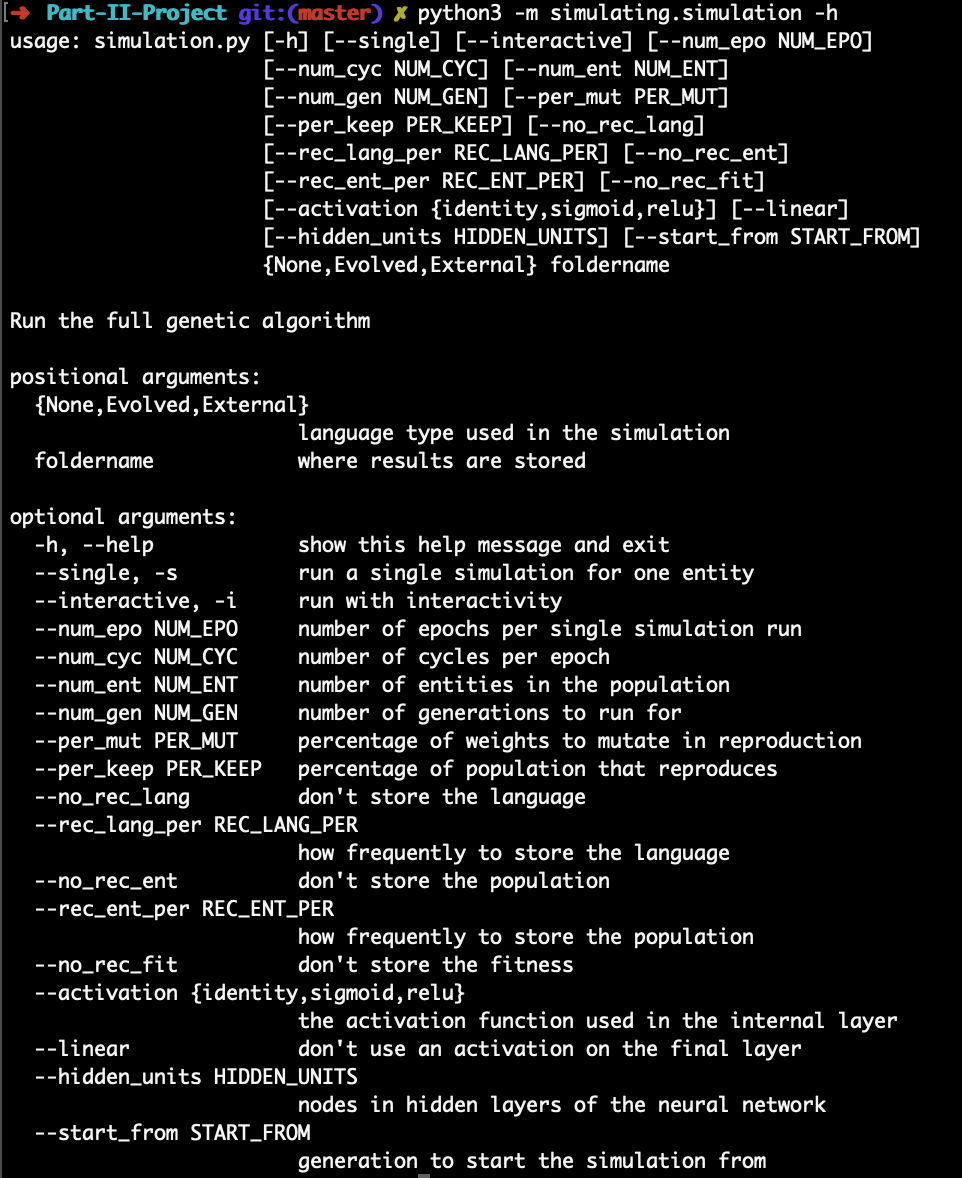
\includegraphics[width=1.\linewidth]{figs/commandline}
          \caption{Result of running \texttt{python3 -m simulating.simulation -h} to display the help page for the command-line interface of the simulation module. The required parameters are the foldername (for storing results) and the language type, all other parameters have a default value.}
      \label{fig:commandline}
   \end{minipage}
   \begin{minipage}{0.49\textwidth}
          \centering
          \captionsetup{width=.9\linewidth}
          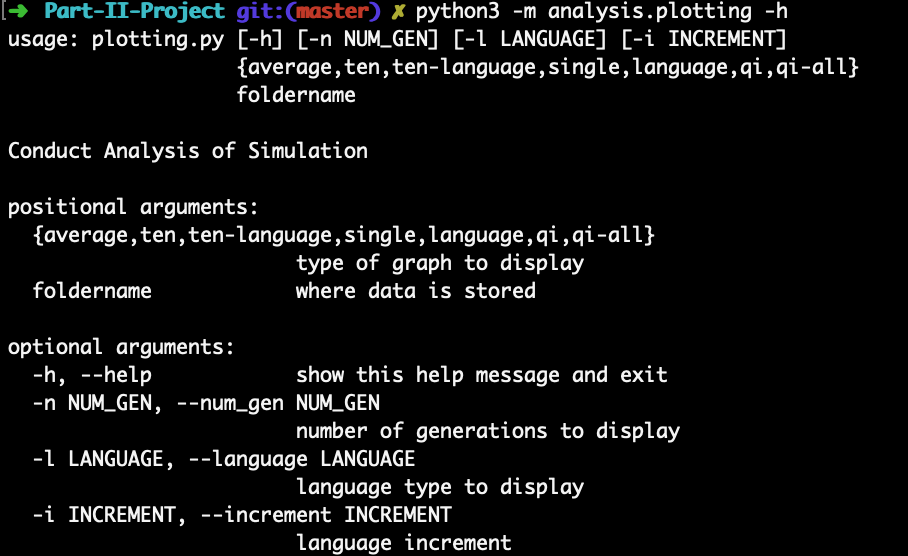
\includegraphics[width=1.\linewidth]{figs/commandline2}
          \caption{Result of running \texttt{python3 -m analysis.plotting -h} to display the help page for the command-line interface of the analysis module. The required parameters are the foldername (where the results are found in order to plot) and the type of graph to display.}
      \label{fig:commandline2}
   \end{minipage}
\end{figure*}

Figures \ref{fig:commandline} and \ref{fig:commandline2} present the command-line interface information screens for the simulating and analysis modules respectively; giving the parameters used to configure these processes.

\cref{fig:interactive} shows the result of running an interactive simulation. Each generation is run following a press of ENTER by the user, or $n$ generations will run if the user enters a number $n$. With each generation, the live average fitness graph is updated and the exact fitness score for each entity in the population is displayed as a sorted list in the terminal.

If the user enters \texttt{watch $n$} for some index into the array of entities $n$, this will allow the user to watch a run of the simulation for a particular entity, as seen in \cref{fig:interactivesingle}. This displays the current epoch, cycle number, then a grid representing the world that the entity exists within. Mushrooms as displayed as emojis and the entity is displayed as a triangle with the tip of the triangle giving the direction of the entity. Below this grid, some information about the simulation is given along with the inputs passed to the \texttt{behaviour()} method and the outputs received.

\begin{figure}[ht]
  \centering
  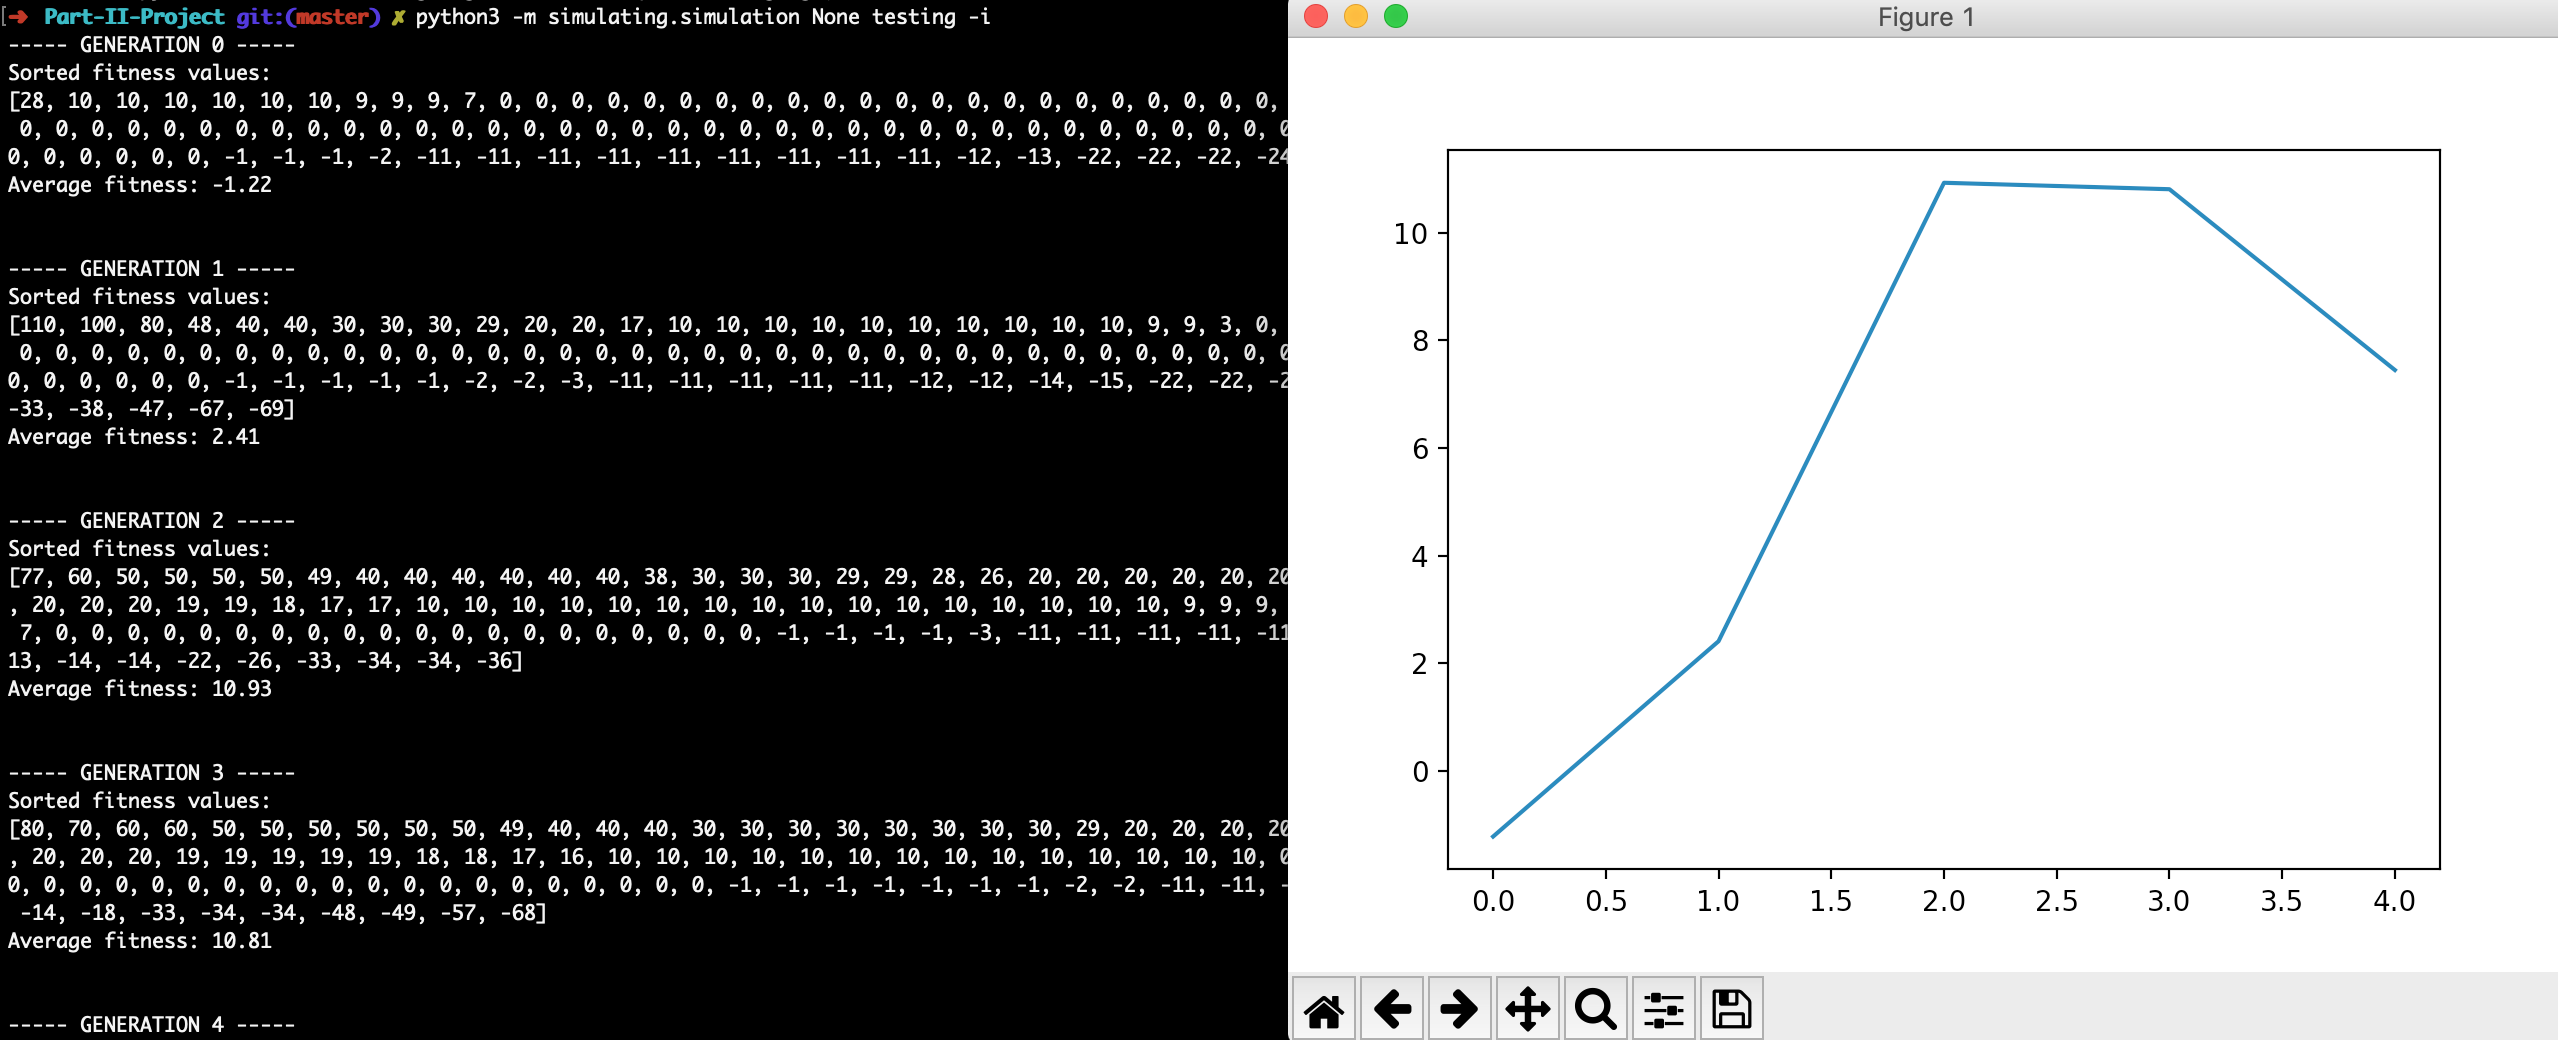
\includegraphics[width=.9\linewidth]{figs/interactive}
  \caption{Visualisation of running a default simulation for a {\bf no language} population using the interactivity flag (\texttt{-i}). The left side shows the terminal output and the right side shows the live fitness graph.}
  \label{fig:interactive}
\end{figure}

\begin{figure}[ht]
  \centering
  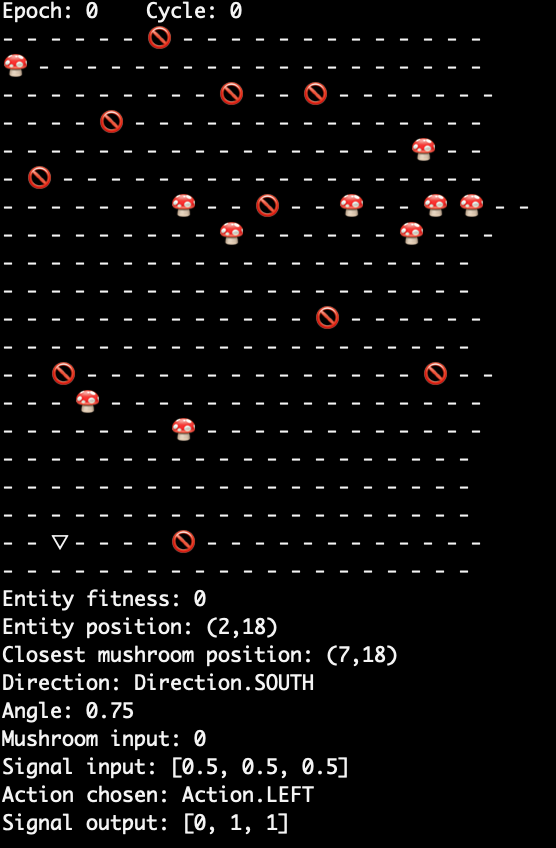
\includegraphics[width=.9\linewidth]{figs/interactivesingle}
  \caption{Visualisation of watching the behaviour of a single entity in a population, selected from an interactive simulation by entering \texttt{watch 0}.}
  \label{fig:interactivesingle}
\end{figure}


\chapter{Project Proposal}

\documentclass[12pt]{article}
\usepackage{a4wide}
\usepackage{datetime}
\usepackage{url}
\usepackage{hyperref}
\usepackage[svgnames]{xcolor}
\hypersetup{
  colorlinks,
  urlcolor=Blue}

\newcommand{\al}{$<$}
\newcommand{\ar}{$>$}
\newcommand{\sups}{\textsuperscript}
\newcommand{\belgianspacing}{\frenchspacing}

\parindent 0pt
\parskip 6pt

\begin{document}

\belgianspacing

\thispagestyle{empty}

%\rightline{\large\emph{Z\'ebulon Goriely}}
%\medskip
%\rightline{\large\emph{Queens'}}
%\medskip
%\rightline{\large\emph{zg258}}

%\vfil

\centerline{\large Computer Science Part II Project Proposal}
\vspace{0.2in}
\centerline{\Large\bf Simulating Language Learning and Evolution}
\vspace{0.2in}
\centerline{\large {\bf{Z\'ebulon Goriely --- Queens' --- zg258}}}
\vspace{0.2in}
\newdate{proposaldate}{18}{10}{2019}
\centerline{\large {\displaydate{proposaldate}}}
 
 \vspace{0.3in}
 
%\vfil

{\bf Project Originator:} Z\'ebulon Goriely

{\bf Project Supervisor:} {Prof. Paula Buttery and Dr. Andrew Caines}

{\bf Director of Studies:}  {Prof. Alastair Beresford}

{\bf Overseers:} {Prof. Pietro Lio’} and {Dr. Robert Mullins}

\section*{Introduction}

Language has evolved and therefore probably gave an evolutionary advantage to the individuals that exhibited it. As Angelo Cangelosi and Domenico Parisi described in a 1998 paper\footnote{\url{https://doi.org/10.1080/095400998116512}}, it is difficult to investigate the evolutionary origin of language and the selective pressures that may have originated language due to the limited evidence available. They propose using computer simulations of evolutionary scenarios to investigate this. In the paper referenced, they describe a simulated toy world where agents controlled by neural-networks interact with an environment of mushrooms that are edible and poisonous. This simulation and the ideas explored in the paper will be the basis for my project.

In the paper, Cangelosi and Parisi use small feed-forward neural networks to control the behaviour of each agent. The weights are initially random; a genetic algorithm is used to improve the fitness of the species over many generations. The agents are also given linguistic abilities; input and output nodes of the neural networks produce signals that allow for communication.

By creating three different populations (one without language, one with an externally imposed language and one with an evolved language) we can investigate the evolutionary advantage of language. Furthermore, it allows us to investigate a key question posed in the paper: \emph{``Since language requires the parallel evolution of linguistic production and linguistic comprehension, how can language evolve when it has a purely informative function and therefore it is advantageous to the receiver but not the producer?''}

For this project, I will re-implement the simulation described. I will then create analysis tools to investigate the findings of the paper to see if I observe the same results.

\section*{Starting Point}

I have a small amount of experience in programming simulations; for my A-Level project in 2016, I created a simulation of virus propogation between mosquito and human agents in the Unity game engine.

I do not have any experience programming neural networks, however, I am confident that I understand the backpropagation algorithm and basic neural network structure through the Artificial Intelligence course I took last year. In the papers I plan to reference, Cangelosi very clearly describes the structure of the neural networks he uses and I am confident that I will be able to follow his work.

Over the summer I read a book titled Simulating the Evolution of Language which gave me an overview of the techniques used in this field. Alongside the Formal Models of Language course that I took last year, I now have a sufficient base of understanding to begin this project.

\section*{Work to be Done}

The work for this project can be roughly divided into two stages; implementing the simulation and constructing the means of evaluating my implementation against the findings in the original paper. I will also regularly be creating tests to evaluate my simulation.

\subsection*{Implementing the Simulation}

\begin{enumerate}

\item Set up the simulation environment by creating the world grid and implementing the properties of poisonous and edible mushrooms. Create the simulation loop divided into regular `epochs'.

\item Create the agents for the simulation, giving them position and energy properties.

\item Implement feedforward neural networks to control the behaviour of the agents; input units to identify the location of the nearest mushroom, visual perception units to observe mushroom properties (only when close enough) and signal perception units for when language is implemented. The output units control the movement of the agent and production of signals. There will also be hidden units.

\item Implement the genetic algorithm that runs after all agents complete the simulation. The fittest agents are determined by the energy level (based on eating edible mushrooms and avoiding poisonous mushrooms). The fittest agents are then chosen for asexual reproduction, producing offspring that have genetic mutations in the form selecting a percentage of the weights to change by a random amount.

\item Create two different populations, one without language (where the signal perception units are always set to the same, constant value) and one with an externally imposed language (where the signal perception units are set to one of two signals depending on the type of the nearest mushroom).

\item Create a third population with an evolved language. Instead of externally imposed signals, in each simulation cycle one of the other agents is randomly selected as the `speaker' and its output is connected to the input signal perception units of the `listener'. 

\end{enumerate}

\subsection*{Analysis}

\begin{enumerate}

\item Plot the average fitness over the number of generations to compare between the three populations.

\item Produce some behavioural tests to investigate the behaviour of random individual organisms at specific generations.

\item Plot the frequency distribution of the different signals produced by the individuals with the evolved language using a `naming task'.

\item Calculate the Quality Index (QI) of the language produced by the population without language and the population with an evolved language to investigate the genetic advantage of producing productive signals. The QI evaluates the efficiency of a language based off of three criteria; (1) functionally distinct categories are labeled with distinct signals, (2) a single signal tends to be used to label all the instances within a category and (3) all the individuals in the population tend to use the same signal to label the same category.

\item Investigate the correlation between QI of the language and the fitness of the species to determine if change in the language or in the categorisation skill of the agents affects the other ability.

\end{enumerate}

\subsection*{Testing}

To evaluate my project and ensure that my simulation implementation is functional, I will create an ensemble of unit tests for each of the tasks above. These will be created in parallel as I develop each part of the implementation. For the simulation, this will involve small examples or scenarios to show that each part of the simulation is fully functional.

\section*{Success Criterion}

The project will be deemed a success if I can implement the simulation as described in the tasks above (evaluated by my unit tests) and if I can implement the analysis tools to compare the findings of my implementation to the findings of the original paper.

\section*{Timetable and Milestones}

I've broken down this timetable into two and three week intervals. At the end of December, I will be writing my Progress Report and simultaneously making adjustments to the timetable as needed.

\subsection*{25\sups{th} October -- 10\sups{th} November}

\emph{Middle of Michaelmas Term. Includes first deadline for NLP coursework.}


{\bf Task:} Create a high-level design of the system. Set up the project files with a version-control system. Experiment with creating small simulations in python and do suitable research into Neural Network libraries.

{\bf Milestones:} Have a git repository with project files. Have a design plan with specific details of the simulation confirmed.

\subsection*{11\sups{th} November -- 24\sups{th} November}

\emph{Middle of Michaelmas Term.}


{\bf Task:} Complete implementation tasks 1 and 2 as described above. Experiment with adding Neural Networks to control the behaviour of the agents.

{\bf Milestones:} Have a working simulation environment with poisonous and edible mushrooms. Have agents with positions and energy values but no functional neural networks yet.

\subsection*{25\sups{th} November -- 8\sups{th} December}

\emph{End of Michaelmas Term. Includes second and third deadline for NLP coursework.}


{\bf Task:} Complete implementation tasks (3). Start working on implementation task (4).

{\bf Milestones:} Have the agents successfully controlled by neural networks. Be able to run an entire lifespan of one agent within the simulated world. Have the beginnings of a 

\subsection*{9\sups{th} December -- 22\sups{nd} December}

\emph{Christmas holiday. Will likely be in Cambridge to help with Queens' interviews.}

{\bf Task:} Complete implementation tasks (4), (5) and (6). Also aim to complete analysis tasks (1) and (3).

{\bf Milestones:} Have a fully functional simulation that allows for running a thousand generations of a population of agents. Have three different populations to compare; one without language, one with an externally imposed language and one with an evolved language. Have a tool to graph the average fitness of each population over the number of generations and another tool to view the probability distribution of the signals chosen for the evolved language over the number of generations.

\subsection*{23\sups{rd} December -- 12\sups{th} January}

\emph{Christmas holiday. Will take a break to revise Michaelmas courses and to spend time with family.}

{\bf Task:} Complete analysis task (2). Write the Preparation chapter of the Dissertation. Review the timetable for the remainder of the project and adjust in light of experience so far. If ahead of schedule, plan time for extensions. Start to plan tests cases.

{\bf Milestones:} An outline of the dissertation document with a completed Preparation section.

\subsection*{13\sups{th} January -- 2\sups{nd} February}

\emph{Start of Lent term. Will have regular labs for Mobile Robot Systems.}

{\bf Progress Report Deadline:} 31\sups{st} January

{\bf Task:} Write the Progress Report. Start to fill out the Implementation chapter of the Dissertation. Complete analysis tasks (4) and (5).

{\bf Milestones:} Progress report submitted and entired project reviewed both personally and with overseers. Have tools to plot the Quality Index of the evolved language against the fitness of the population. At this point, all the tasks in the {\bf Work to Do} section will have been completed, satisfying the {\bf Success Criteria}.

\subsection*{3\sups{rd} February -- 23\sups{rd} February}

\emph{Middle of Lent term. Both deadlines for the Mobile Robot Systems assignments.}

{\bf Task:} Begin analysis of the simulation. Begin to work on extensions to the project, keeping in mind time needed to write the Dissertation.

{\bf Milestones:} Have the start of a test suite with a series of diagrams to use to evaluate my implementation.

\subsection*{24\sups{th} February -- 15\sups{th} March}

\emph{End of Lent term. Deadline for the Mobile Robot Systems mini-project report.}

{\bf Task:} Complete testing. Evaluate the outcomes of the tests against the findings in the original paper. At this point, the second half of the {\bf Success Criteria} will have been achieved. If needed, revise the implementation to be clean, documented and consise. Work on other extensions.

{\bf Milestones:} Examples and test cases run with results collected. Code should perform a variety of interesting tasks and should be in a state that in the worst case it would satisfy the examiners with at most cosmetic adjustment

\subsection*{16\sups{th} March -- 5\sups{th} April}

\emph{Start of Easter holiday. Might stay in Cambridge for part of it to work. Will balance revision and work on the project.}

{\bf Task:} Complete work on any extensions. Draft the Evaluations and Conclusions chapters of the Dissertation.

{\bf Milestones:} Extensions almost complete. Skeleton of entire Dissertation in place.

\subsection*{6\sups{th} April -- 19\sups{th} April}

\emph{End of Easter holiday. Might get back to Cambridge early to work. Will balance revision and work on the project.}

{\bf Task:} Complete the Implementation and Introduction chapters of the Dissertation. Send the full draft to Director of Studies and Supervisors by 21st of April.

{\bf Milestones:} Dissertation essentially complete, with large sections of it proof-read by Supervisors and possibly friends and/or Director of Studies.

\subsection*{20\sups{th} April -- 8\sups{th} May}

\emph{Start of Easter Term. Will be balancing revision, lectures and final work on the project.}

{\bf Final Deadline:} 8\sups{th} May

{\bf Task:} Finish Dissertation, preparing diagrams for insertion. Review the whole project, checking the Dissertation and spending the final few days on whatever is in greatest need of attention. Aim to submit the dissertation at least a week before the deadline.

{\bf Milestone:} Submission of Dissertation

\section*{Possible Extensions}

\subsection*{Graphic Visualisation}

As a side extension, I could implement a visual interface to watch the life of one agent within the simulation. This would involve rendering a simple 2D world with textures for the agents and mushrooms. This could be expanded further by adding a User Interface for setting up the simulation and having windows showing the progress as it occurs live.

\subsection*{Symbolic Theft vs. Sensorimotor Toil}

In a 2000 paper\footnote{\url{http://cogprints.org/2036/}}, Cangelosi and Harnad use a similar same toy world of mushrooms and foragers to place two ways of acquiring categories in direct competition with each other. They compare ``sensorimotor toil'' (where categories are acquired through real-time, feedback-correct, trial and error experience) to ``symbolic theft'' (where new categories are acquired by hearsay from boolean combinations of symbols \emph{describing} them). They find that the origins of natural language could be explained by the apparent infinitely superiority of a hybrid symbolic/sensorimotor combination compared to purely sensorimotor precursors. 

As an extension, I could expand my simulation to investigate the findings of this paper. This involves implementing a more complicated neural network, adding supervised learning through back-propagation, implementing more sophisticated mushroom features and expanding the simulation to host multiple populations at once.

\subsection*{Investigating the Evolution of Syntax}

In a 1999 paper\footnote{\url{https://link.springer.com/chapter/10.1007/3-540-48304-7_86}}, Cangelosi expands the toy mushroom world simulation further to investigate how languages that use combinations of words (such as the ``verb-object'' rule) can emerge by auto-organisation and cultural transmission. Mushrooms are either edible or poisonous but also have one of three colours - the edible mushrooms of a particular colour correspond to a particular action in response.

In this extended simulation, after the first 300 generations parents and children co-exist within the simulated world. Parents teach the evolved language to their children. Children undergo a Listening Task (where parents describe the closest mushroom) and a Naming Task (where the mushroom name is used for supervised learning through backpropagation).

This is a substantial increase in complexity but allows would allow me to investigate the evolution of a more complex language.

 \section*{Resources Declaration}

For this project, I plan to use my computer, (2.8 GHz CPU, 16 GB RAM, 750GB Flash Storage,
macOS Mojave). The code will be regularly pushed to a GitHub repository to be able to recover from failure or loss on my local machine. I will also create weekly backups on an external hard-drive to provide another source of recovery. Should my machine fail, I will be able to continue working on an MCS machine. I accept full responsibility for this machine and I have made contingency plans to protect myself against hardware and/or software failure. 

I will also need to use the high powered computer when running large simulations to save processing time.

 \end{document}



%TC:endignore
\end{document}
